\documentclass[twoside]{book}

% Packages required by doxygen
\usepackage{calc}
\usepackage{doxygen}
\usepackage{graphicx}
\usepackage[utf8]{inputenc}
\usepackage{makeidx}
\usepackage{multicol}
\usepackage{multirow}
\usepackage{textcomp}
\usepackage[table]{xcolor}

% Font selection
\usepackage[T1]{fontenc}
\usepackage{mathptmx}
\usepackage[scaled=.90]{helvet}
\usepackage{courier}
\usepackage{amssymb}
\usepackage{sectsty}
\renewcommand{\familydefault}{\sfdefault}
\allsectionsfont{%
  \fontseries{bc}\selectfont%
  \color{darkgray}%
}
\renewcommand{\DoxyLabelFont}{%
  \fontseries{bc}\selectfont%
  \color{darkgray}%
}

% Page & text layout
\usepackage{geometry}
\geometry{%
  a4paper,%
  top=2.5cm,%
  bottom=2.5cm,%
  left=2.5cm,%
  right=2.5cm%
}
\tolerance=750
\hfuzz=15pt
\hbadness=750
\setlength{\emergencystretch}{15pt}
\setlength{\parindent}{0cm}
\setlength{\parskip}{0.2cm}
\makeatletter
\renewcommand{\paragraph}{%
  \@startsection{paragraph}{4}{0ex}{-1.0ex}{1.0ex}{%
    \normalfont\normalsize\bfseries\SS@parafont%
  }%
}
\renewcommand{\subparagraph}{%
  \@startsection{subparagraph}{5}{0ex}{-1.0ex}{1.0ex}{%
    \normalfont\normalsize\bfseries\SS@subparafont%
  }%
}
\makeatother

% Headers & footers
\usepackage{fancyhdr}
\pagestyle{fancyplain}
\fancyhead[LE]{\fancyplain{}{\bfseries\thepage}}
\fancyhead[CE]{\fancyplain{}{}}
\fancyhead[RE]{\fancyplain{}{\bfseries\leftmark}}
\fancyhead[LO]{\fancyplain{}{\bfseries\rightmark}}
\fancyhead[CO]{\fancyplain{}{}}
\fancyhead[RO]{\fancyplain{}{\bfseries\thepage}}
\fancyfoot[LE]{\fancyplain{}{}}
\fancyfoot[CE]{\fancyplain{}{}}
\fancyfoot[RE]{\fancyplain{}{\bfseries\scriptsize Generated on Sun Jun 12 2016 20\-:56\-:15 for Family Tree by Doxygen }}
\fancyfoot[LO]{\fancyplain{}{\bfseries\scriptsize Generated on Sun Jun 12 2016 20\-:56\-:15 for Family Tree by Doxygen }}
\fancyfoot[CO]{\fancyplain{}{}}
\fancyfoot[RO]{\fancyplain{}{}}
\renewcommand{\footrulewidth}{0.4pt}
\renewcommand{\chaptermark}[1]{%
  \markboth{#1}{}%
}
\renewcommand{\sectionmark}[1]{%
  \markright{\thesection\ #1}%
}

% Indices & bibliography
\usepackage{natbib}
\usepackage[titles]{tocloft}
\setcounter{tocdepth}{3}
\setcounter{secnumdepth}{5}
\makeindex

% Hyperlinks (required, but should be loaded last)
\usepackage{ifpdf}
\ifpdf
  \usepackage[pdftex,pagebackref=true]{hyperref}
\else
  \usepackage[ps2pdf,pagebackref=true]{hyperref}
\fi
\hypersetup{%
  colorlinks=true,%
  linkcolor=blue,%
  citecolor=blue,%
  unicode%
}

% Custom commands
\newcommand{\clearemptydoublepage}{%
  \newpage{\pagestyle{empty}\cleardoublepage}%
}


%===== C O N T E N T S =====

\begin{document}

% Titlepage & ToC
\hypersetup{pageanchor=false}
\pagenumbering{roman}
\begin{titlepage}
\vspace*{7cm}
\begin{center}%
{\Large Family Tree \\[1ex]\large 0.\-2 }\\
\vspace*{1cm}
{\large Generated by Doxygen 1.8.6}\\
\vspace*{0.5cm}
{\small Sun Jun 12 2016 20:56:15}\\
\end{center}
\end{titlepage}
\clearemptydoublepage
\tableofcontents
\clearemptydoublepage
\pagenumbering{arabic}
\hypersetup{pageanchor=true}

%--- Begin generated contents ---
\chapter{2.0 B\-O\-O\-T\-S\-T\-R\-A\-P J\-S P\-H\-I\-L\-O\-S\-O\-P\-H\-Y}
\label{md_assets_js_README}
\hypertarget{md_assets_js_README}{}
These are the high-\/level design rules which guide the development of Bootstrap's plugin apis. 



\subsubsection*{D\-A\-T\-A-\/\-A\-T\-T\-R\-I\-B\-U\-T\-E A\-P\-I}

We believe you should be able to use all plugins provided by Bootstrap purely through the markup A\-P\-I without writing a single line of javascript.

We acknowledge that this isn't always the most performant and sometimes it may be desirable to turn this functionality off altogether. Therefore, as of 2.\-0 we provide the ability to disable the data attribute A\-P\-I by unbinding all events on the body namespaced with {\ttfamily 'data-\/api'}. This looks like this\-: \begin{DoxyVerb}$('body').off('.data-api')
\end{DoxyVerb}


To target a specific plugin, just include the plugins name as a namespace along with the data-\/api namespace like this\-: \begin{DoxyVerb}$('body').off('.alert.data-api')
\end{DoxyVerb}






\subsubsection*{P\-R\-O\-G\-R\-A\-M\-A\-T\-I\-C A\-P\-I}

We also believe you should be able to use all plugins provided by Bootstrap purely through the J\-S A\-P\-I.

All public A\-P\-Is should be single, chainable methods, and return the collection acted upon. \begin{DoxyVerb}$(".btn.danger").button("toggle").addClass("fat")
\end{DoxyVerb}


All methods should accept an optional options object, a string which targets a particular method, or null which initiates the default behavior\-: \begin{DoxyVerb}$("#myModal").modal() // initialized with defaults
$("#myModal").modal({ keyboard: false }) // initialized with now keyboard
$("#myModal").modal('show') // initializes and invokes show immediately afterqwe2
\end{DoxyVerb}






\subsubsection*{O\-P\-T\-I\-O\-N\-S}

Options should be sparse and add universal value. We should pick the right defaults.

All plugins should have a default object which can be modified to effect all instance's default options. The defaults object should be available via {\ttfamily \$.fn.\-plugin.\-defaults}. \begin{DoxyVerb}$.fn.modal.defaults = { … }
\end{DoxyVerb}


An options definition should take the following form\-: \begin{DoxyVerb}*noun*: *adjective* - describes or modifies a quality of an instance
\end{DoxyVerb}


examples\-: \begin{DoxyVerb}backdrop: true
keyboard: false
placement: 'top'
\end{DoxyVerb}






\subsubsection*{E\-V\-E\-N\-T\-S}

All events should have an infinitive and past participle form. The infinitive is fired just before an action takes place, the past participle on completion of the action. \begin{DoxyVerb}show | shown
hide | hidden
\end{DoxyVerb}






\subsubsection*{C\-O\-N\-S\-T\-R\-U\-C\-T\-O\-R\-S}

Each plugin should expose it's raw constructor on a {\ttfamily Constructor} property -- accessed in the following way\-:

\begin{DoxyVerb}$.fn.popover.Constructor
\end{DoxyVerb}






\subsubsection*{D\-A\-T\-A A\-C\-C\-E\-S\-S\-O\-R}

Each plugin stores a copy of the invoked class on an object. This class instance can be accessed directly through j\-Query's data A\-P\-I like this\-: \begin{DoxyVerb}$('[rel=popover]').data('popover') instanceof $.fn.popover.Constructor
\end{DoxyVerb}






\subsubsection*{D\-A\-T\-A A\-T\-T\-R\-I\-B\-U\-T\-E\-S}

Data attributes should take the following form\-:


\begin{DoxyItemize}
\item data-\/\{\{verb\}\}=\{\{plugin\}\} -\/ defines main interaction
\item data-\/target $\vert$$\vert$ href$^\wedge$=\# -\/ defined on \char`\"{}control\char`\"{} element (if element controls an element other than self)
\item data-\/\{\{noun\}\} -\/ defines class instance options
\end{DoxyItemize}

examples\-: \begin{DoxyVerb}// control other targets
data-toggle="modal" data-target="#foo"
data-toggle="collapse" data-target="#foo" data-parent="#bar"

// defined on element they control
data-spy="scroll"

data-dismiss="modal"
data-dismiss="alert"

data-toggle="dropdown"

data-toggle="button"
data-toggle="buttons-checkbox"
data-toggle="buttons-radio" \end{DoxyVerb}
 
\chapter{\mbox{[}Family\-Tree\mbox{]}(http\-://vanshavali.ratupar.\-in)}
\label{md_README}
\hypertarget{md_README}{}
$\ast$$\ast$\href{http://vanshavali.ratupar.in}{\tt Family\-Tree}$\ast$$\ast$ is simple P\-H\-P Application targetting the collection of family data which can viewed with beautiful visualisation. You can add/update data, play with the visualisation, show you children their roots, add new members as they enter your family.

\section*{Installation }


\begin{DoxyEnumerate}
\item First thing is to clone the repository. If you are not familiar with the word clone, it just means to download the application. You can download it from \href{https://github.com/piyushparkash/FamilyTree/archive/develop.zip}{\tt here}, else if you know how to clone, below is the command you can use to clone the repository. \begin{DoxyVerb} $ git clone https://github.com/piyushparkash/FamilyTree.git
\end{DoxyVerb}

\item After this step you have to move the url of the server where you have place the source after the first step. Let's assume that you are installing this application locally say in /var/www/\-Family\-Tree. Then go to {\ttfamily localhost/\-Family\-Tree}.
\item After this if you see output from the browser apart from 404 Not Found error, then you are in right path. You must see something saying, Please provide permissions to some directories. Please use the below command to give permission \begin{DoxyVerb} $ chmod -R 744 directory_name/
\end{DoxyVerb}

\end{DoxyEnumerate}

Few directories in Family\-Tree need write permissions which are not there by default. You will have to provide that explicitly.


\begin{DoxyEnumerate}
\item After the 3rd step it's pretty much self explainatory. But if you still need help, I am mentioning the steps. First thing that {\bfseries Family\-Tree} will be doing would be to setup the database. So you need to provide the database credentials. I am mentioning the default values. It might be different in your systems.

{\ttfamily Host\-: localhost}

{\ttfamily Username\-: root}

{\ttfamily Password\-: your-\/password}

{\ttfamily Database\-: mention any name}
\end{DoxyEnumerate}

5) If everything goes right, It will install Family\-Tree with sample data in it and you will be able to see the Family with the visualisation.

\subsection*{Facing Problems? }

We are so sorry that you are facing problems.

Report it \href{https://github.com/piyushparkash/FamilyTree/issues}{\tt here} so that we can act on it immediately.

\subsection*{Get Involved / Contribute }

Visit this \href{http://vanshavali.ratupar.in}{\tt website}

\subsection*{A\-U\-T\-H\-O\-R\-S\-: }

Piyush Parkash

Official Website\-: \href{http://vanshavali.ratupar.in}{\tt vanshavali.\-ratupar.\-in}

Email\-: \href{mailto:achyutapiyush@gmail.com}{\tt achyutapiyush@gmail.\-com} 
\chapter{Namespace Index}
\section{Namespace List}
Here is a list of all documented namespaces with brief descriptions\-:\begin{DoxyCompactList}
\item\contentsline{section}{\hyperlink{namespacedb}{db} }{\pageref{namespacedb}}{}
\item\contentsline{section}{\hyperlink{namespaceinstall}{install} }{\pageref{namespaceinstall}}{}
\end{DoxyCompactList}

\chapter{Hierarchical Index}
\section{Class Hierarchy}
This inheritance list is sorted roughly, but not completely, alphabetically\-:\begin{DoxyCompactList}
\item \contentsline{section}{adminuser}{\pageref{classadminuser}}{}
\item \contentsline{section}{auth}{\pageref{classauth}}{}
\begin{DoxyCompactList}
\item \contentsline{section}{user}{\pageref{classuser}}{}
\item \contentsline{section}{user}{\pageref{classuser}}{}
\end{DoxyCompactList}
\item \contentsline{section}{db}{\pageref{classdb}}{}
\item \contentsline{section}{install}{\pageref{classinstall}}{}
\item member\-\_\-operation\-\_\-suggest\begin{DoxyCompactList}
\item \contentsline{section}{member\-\_\-operation}{\pageref{classmember__operation}}{}
\begin{DoxyCompactList}
\item \contentsline{section}{member}{\pageref{classmember}}{}
\item \contentsline{section}{member}{\pageref{classmember}}{}
\end{DoxyCompactList}
\item \contentsline{section}{member\-\_\-operation}{\pageref{classmember__operation}}{}
\item \contentsline{section}{suggest}{\pageref{classsuggest}}{}
\item \contentsline{section}{suggest}{\pageref{classsuggest}}{}
\end{DoxyCompactList}
\item \contentsline{section}{module}{\pageref{classmodule}}{}
\item \contentsline{section}{suggest\-\_\-handler}{\pageref{classsuggest__handler}}{}
\item \contentsline{section}{suggest\-\_\-storage}{\pageref{classsuggest__storage}}{}
\item \contentsline{section}{suggestion}{\pageref{classsuggestion}}{}
\item \contentsline{section}{vanshavali}{\pageref{classvanshavali}}{}
\end{DoxyCompactList}

\chapter{Class Index}
\section{Class List}
Here are the classes, structs, unions and interfaces with brief descriptions\-:\begin{DoxyCompactList}
\item\contentsline{section}{\hyperlink{classadminuser}{adminuser} }{\pageref{classadminuser}}{}
\item\contentsline{section}{\hyperlink{classauth}{auth} }{\pageref{classauth}}{}
\item\contentsline{section}{\hyperlink{classdb}{db} }{\pageref{classdb}}{}
\item\contentsline{section}{\hyperlink{classinstall}{install} }{\pageref{classinstall}}{}
\item\contentsline{section}{\hyperlink{classmember}{member} }{\pageref{classmember}}{}
\item\contentsline{section}{\hyperlink{classmember__operation}{member\-\_\-operation} }{\pageref{classmember__operation}}{}
\item\contentsline{section}{\hyperlink{classmodule}{module} }{\pageref{classmodule}}{}
\item\contentsline{section}{\hyperlink{classsuggest}{suggest} }{\pageref{classsuggest}}{}
\item\contentsline{section}{\hyperlink{classsuggest__handler}{suggest\-\_\-handler} }{\pageref{classsuggest__handler}}{}
\item\contentsline{section}{\hyperlink{classsuggest__storage}{suggest\-\_\-storage} }{\pageref{classsuggest__storage}}{}
\item\contentsline{section}{\hyperlink{classsuggestion}{suggestion} }{\pageref{classsuggestion}}{}
\item\contentsline{section}{\hyperlink{classuser}{user} }{\pageref{classuser}}{}
\item\contentsline{section}{\hyperlink{classvanshavali}{vanshavali} }{\pageref{classvanshavali}}{}
\end{DoxyCompactList}

\chapter{Namespace Documentation}
\hypertarget{namespacedb}{\section{db Namespace Reference}
\label{namespacedb}\index{db@{db}}
}


\subsection{Detailed Description}
This class handles all the interaction with the database

\begin{DoxyAuthor}{Author}
piyush 
\end{DoxyAuthor}

\hypertarget{namespaceinstall}{\section{install Namespace Reference}
\label{namespaceinstall}\index{install@{install}}
}


\subsection{Detailed Description}
This class contains function to install Family Tree

\begin{DoxyAuthor}{Author}
piyush 
\end{DoxyAuthor}

\chapter{Class Documentation}
\hypertarget{classadminuser}{\section{adminuser Class Reference}
\label{classadminuser}\index{adminuser@{adminuser}}
}
\subsection*{Public Member Functions}
\begin{DoxyCompactItemize}
\item 
\hypertarget{classadminuser_a023621037bd64b0fc4f28bb051d0eaf9}{{\bfseries \-\_\-\-\_\-construct} (\$getvars, \$template, \$\hyperlink{classdb}{db})}\label{classadminuser_a023621037bd64b0fc4f28bb051d0eaf9}

\end{DoxyCompactItemize}
\subsection*{Public Attributes}
\begin{DoxyCompactItemize}
\item 
\hypertarget{classadminuser_a13271febb31a709aa5a26f5069c15acc}{{\bfseries \$database}}\label{classadminuser_a13271febb31a709aa5a26f5069c15acc}

\end{DoxyCompactItemize}
\subsection*{Protected Attributes}
\begin{DoxyCompactItemize}
\item 
\hypertarget{classadminuser_aaa7c2068ee100d11b2cdaecf5ca9bcf9}{{\bfseries \$templateholder}}\label{classadminuser_aaa7c2068ee100d11b2cdaecf5ca9bcf9}

\end{DoxyCompactItemize}


\subsection{Detailed Description}


Definition at line 3 of file adminuser.\-php.



The documentation for this class was generated from the following file\-:\begin{DoxyCompactItemize}
\item 
admin/mods/adminuser.\-php\end{DoxyCompactItemize}

\hypertarget{classauth}{\section{auth Class Reference}
\label{classauth}\index{auth@{auth}}
}
Inheritance diagram for auth\-:\begin{figure}[H]
\begin{center}
\leavevmode
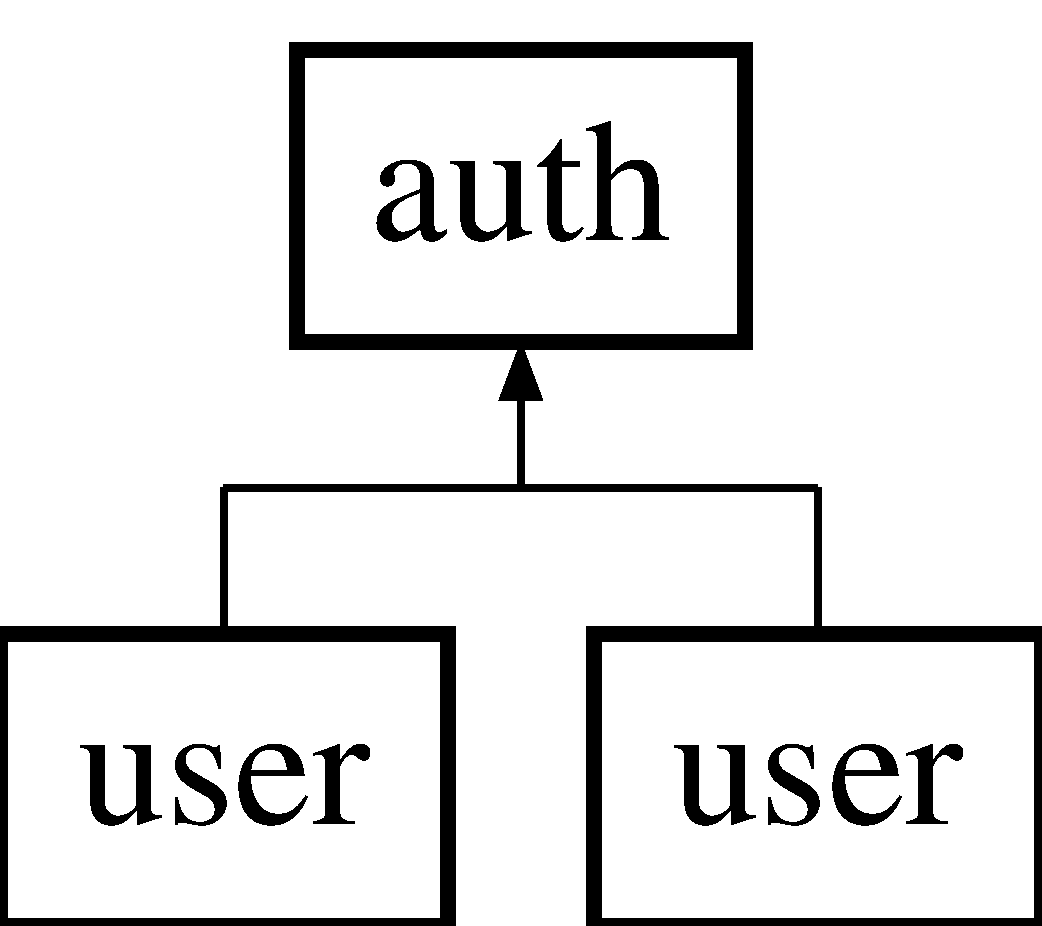
\includegraphics[height=2.000000cm]{classauth}
\end{center}
\end{figure}
\subsection*{Public Member Functions}
\begin{DoxyCompactItemize}
\item 
\hyperlink{classauth_a476f6d06e1ddb49cf4268918363c1d99}{\-\_\-\-\_\-construct} ()
\item 
\hyperlink{classauth_a019d664334a621e770043d9fb4210836}{authenticate} (\$username, \$password)
\item 
\hyperlink{classauth_a0de1d4416c9fb04b4223cd7a3dd3a623}{user\-\_\-account\-\_\-activated} (\$id)
\item 
\hyperlink{classauth_aebf5c1995f3314883dc475628db61ccc}{get\-\_\-user} (\$id)
\item 
\hyperlink{classauth_ad5c908efc480a57e5625131348f4bf29}{check\-\_\-session} ()
\item 
\hyperlink{classauth_ac2530bf2bba79e22de7e2f3ebb63be3a}{check\-\_\-token} (\$id, \$token)
\item 
\hyperlink{classauth_a73a5af5d9e12014687cf0d360f5e6356}{is\-\_\-authenticated} ()
\item 
\hyperlink{classauth_a4ec05ca8231cd1151246b127f168d457}{generate\-\_\-token} (\$id= '')
\item 
\hyperlink{classauth_adeb7a80afb02aceb540c541d591baf69}{destroy\-\_\-session} ()
\item 
\hyperlink{classauth_a17089bfa7c3b9d0546f80ac9472dfc7b}{unauthenticate} ()
\end{DoxyCompactItemize}


\subsection{Detailed Description}
This class is used to create and destroy sessions. It also handles User Authentication 
\begin{DoxyParams}{Parameters}
{\em none} & \\
\hline
\end{DoxyParams}
\begin{DoxyAuthor}{Author}
piyush 
\end{DoxyAuthor}


Definition at line 7 of file auth.\-php.



\subsection{Constructor \& Destructor Documentation}
\hypertarget{classauth_a476f6d06e1ddb49cf4268918363c1d99}{\index{auth@{auth}!\-\_\-\-\_\-construct@{\-\_\-\-\_\-construct}}
\index{\-\_\-\-\_\-construct@{\-\_\-\-\_\-construct}!auth@{auth}}
\subsubsection[{\-\_\-\-\_\-construct}]{\setlength{\rightskip}{0pt plus 5cm}auth\-::\-\_\-\-\_\-construct (
\begin{DoxyParamCaption}
{}
\end{DoxyParamCaption}
)}}\label{classauth_a476f6d06e1ddb49cf4268918363c1d99}
The constructor of the class 
\begin{DoxyParams}{Parameters}
{\em null} & \\
\hline
\end{DoxyParams}


Definition at line 13 of file auth.\-php.


\begin{DoxyCode}
13                                   \{
14         session\_start();
15     \}
\end{DoxyCode}


\subsection{Member Function Documentation}
\hypertarget{classauth_a019d664334a621e770043d9fb4210836}{\index{auth@{auth}!authenticate@{authenticate}}
\index{authenticate@{authenticate}!auth@{auth}}
\subsubsection[{authenticate}]{\setlength{\rightskip}{0pt plus 5cm}auth\-::authenticate (
\begin{DoxyParamCaption}
\item[{}]{\$username, }
\item[{}]{\$password}
\end{DoxyParamCaption}
)}}\label{classauth_a019d664334a621e770043d9fb4210836}
This function is used to basically log-\/in the user. It takes username and password combination as parameter and return true if such user is present and authentication process was successfully completed. If no such user is present it returns false   \$db The instance of the the db class  array \$\-\_\-\-S\-E\-S\-S\-I\-O\-N The global Session variable storing all the session data 
\begin{DoxyParams}[1]{Parameters}
string & {\em \$username} & The username of the users to check against \\
\hline
string & {\em \$password} & The password of the user \\
\hline
\end{DoxyParams}
\begin{DoxyReturn}{Returns}
boolean 
\end{DoxyReturn}


Definition at line 29 of file auth.\-php.


\begin{DoxyCode}
29                                                        \{
30         global $db;
31         
32         \textcolor{comment}{//Convert Password in md5 Hash}
33         $password = md5($password);
34         $query = $db->query(\textcolor{stringliteral}{"select * from member where username='$username' and password='$password'"});
35         $row = $db->fetch($query);
36 
37         \textcolor{comment}{//if no row found or if user's account is not activated yet then}
38         \textcolor{keywordflow}{if} ($row == \textcolor{keyword}{false}) \{
39             \textcolor{keywordflow}{return} \textcolor{keyword}{false};
40         \}
41         
42         \textcolor{comment}{//Check here for approval if user registration has been approved by the admin. Currently disabled}
43 
44         \textcolor{comment}{//Start the session and start storing data about user}
45         global $\_SESSION;
46         $token = $this->\hyperlink{classauth_a4ec05ca8231cd1151246b127f168d457}{generate\_token}($row[\textcolor{stringliteral}{'id'}]);
47         $\_SESSION[\textcolor{stringliteral}{'membername'}] = $row[\textcolor{stringliteral}{'membername'}];
48         $\_SESSION[\textcolor{stringliteral}{'id'}] = $row[\textcolor{stringliteral}{'id'}];
49         $\_SESSION[\textcolor{stringliteral}{'token'}] = $token;
50         $\_SESSION[\textcolor{stringliteral}{'authenticated'}] = \textcolor{keyword}{true};
51 
52         \textcolor{comment}{//if everything is alright then return true}
53         \textcolor{keywordflow}{return} \textcolor{keyword}{true};
54     \}
\end{DoxyCode}
\hypertarget{classauth_ad5c908efc480a57e5625131348f4bf29}{\index{auth@{auth}!check\-\_\-session@{check\-\_\-session}}
\index{check\-\_\-session@{check\-\_\-session}!auth@{auth}}
\subsubsection[{check\-\_\-session}]{\setlength{\rightskip}{0pt plus 5cm}auth\-::check\-\_\-session (
\begin{DoxyParamCaption}
{}
\end{DoxyParamCaption}
)}}\label{classauth_ad5c908efc480a57e5625131348f4bf29}
This function is used to check if sessions was initialized i.\-e. all the required cookies are set. Return true if set  array \$\-\_\-\-S\-E\-S\-S\-I\-O\-N The Superglobal Session variable \begin{DoxyReturn}{Returns}
boolean 
\end{DoxyReturn}


Definition at line 89 of file auth.\-php.


\begin{DoxyCode}
89                              \{
90         global $\_SESSION;
91         \textcolor{keywordflow}{if} (isset($\_SESSION[\textcolor{stringliteral}{'membername'}], $\_SESSION[\textcolor{stringliteral}{'id'}], $\_SESSION[\textcolor{stringliteral}{'token'}], $\_SESSION[\textcolor{stringliteral}{'authenticated'}])
      ) \{
92             \textcolor{keywordflow}{if} ($\_SESSION[\textcolor{stringliteral}{'authenticated'}] == \textcolor{keyword}{true}) \{
93                 \textcolor{keywordflow}{if} ($this->\hyperlink{classauth_ac2530bf2bba79e22de7e2f3ebb63be3a}{check\_token}($\_SESSION[\textcolor{stringliteral}{'id'}], $\_SESSION[\textcolor{stringliteral}{'token'}])) \{
94                     \textcolor{keywordflow}{return} \textcolor{keyword}{true};
95                 \}
96             \}
97         \}
98 
99         \textcolor{keywordflow}{return} \textcolor{keyword}{false};
100     \}
\end{DoxyCode}
\hypertarget{classauth_ac2530bf2bba79e22de7e2f3ebb63be3a}{\index{auth@{auth}!check\-\_\-token@{check\-\_\-token}}
\index{check\-\_\-token@{check\-\_\-token}!auth@{auth}}
\subsubsection[{check\-\_\-token}]{\setlength{\rightskip}{0pt plus 5cm}auth\-::check\-\_\-token (
\begin{DoxyParamCaption}
\item[{}]{\$id, }
\item[{}]{\$token}
\end{DoxyParamCaption}
)}}\label{classauth_ac2530bf2bba79e22de7e2f3ebb63be3a}
This function is used to checkt the token generated against the user. Return true if matches 
\begin{DoxyParams}[1]{Parameters}
integer & {\em \$id} & The I\-D of the user \\
\hline
string & {\em \$token} & The token generated for the user \\
\hline
\end{DoxyParams}
\begin{DoxyReturn}{Returns}
boolean 
\end{DoxyReturn}


Definition at line 109 of file auth.\-php.


\begin{DoxyCode}
109                                       \{
110         $numtoken = preg\_replace(\textcolor{stringliteral}{"/[^0-9]/"}, \textcolor{stringliteral}{""}, $token);
111         $numtoken = (int) $numtoken;
112         \textcolor{keywordflow}{if} ($numtoken == $id) \{
113 
114             \textcolor{keywordflow}{return} \textcolor{keyword}{true};
115         \} \textcolor{keywordflow}{else} \{
116 
117             \textcolor{keywordflow}{return} \textcolor{keyword}{false};
118         \}
119     \}
\end{DoxyCode}
\hypertarget{classauth_adeb7a80afb02aceb540c541d591baf69}{\index{auth@{auth}!destroy\-\_\-session@{destroy\-\_\-session}}
\index{destroy\-\_\-session@{destroy\-\_\-session}!auth@{auth}}
\subsubsection[{destroy\-\_\-session}]{\setlength{\rightskip}{0pt plus 5cm}auth\-::destroy\-\_\-session (
\begin{DoxyParamCaption}
{}
\end{DoxyParamCaption}
)}}\label{classauth_adeb7a80afb02aceb540c541d591baf69}
This function is used to destroy the session created \begin{DoxyReturn}{Returns}
null 
\end{DoxyReturn}


Definition at line 167 of file auth.\-php.


\begin{DoxyCode}
168     \{
169         session\_unset();
170     \}
\end{DoxyCode}
\hypertarget{classauth_a4ec05ca8231cd1151246b127f168d457}{\index{auth@{auth}!generate\-\_\-token@{generate\-\_\-token}}
\index{generate\-\_\-token@{generate\-\_\-token}!auth@{auth}}
\subsubsection[{generate\-\_\-token}]{\setlength{\rightskip}{0pt plus 5cm}auth\-::generate\-\_\-token (
\begin{DoxyParamCaption}
\item[{}]{\$id = {\ttfamily ''}}
\end{DoxyParamCaption}
)}}\label{classauth_a4ec05ca8231cd1151246b127f168d457}
This function is generated token for a user. Token is a random alphanumeric string 
\begin{DoxyParams}[1]{Parameters}
integer & {\em \$id} & The I\-D of the used to generate the token for. \\
\hline
\end{DoxyParams}
\begin{DoxyReturn}{Returns}
string The generated Token 
\end{DoxyReturn}


Definition at line 140 of file auth.\-php.


\begin{DoxyCode}
140                                       \{
141 
142         $codelenght = 20;
143         \textcolor{keywordflow}{for} ($newcode = \textcolor{stringliteral}{""}, $newcode\_length = 0; $newcode\_length < $codelenght; $newcode\_length++) \{
144             \textcolor{keywordflow}{if} ($newcode\_length == 5) \{
145                 $newcode = $newcode . $id;
146             \}
147             $x = 1;
148             $y = 2;
149             $part = rand($x, $y);
150             \textcolor{keywordflow}{if} ($part == 1) \{
151                 $a = 65;
152                 $b = 90;
153             \} \textcolor{comment}{// UpperCase}
154             \textcolor{keywordflow}{if} ($part == 2) \{
155                 $a = 97;
156                 $b = 122;
157             \} \textcolor{comment}{// LowerCase}
158             $newcode = $newcode . chr(rand($a, $b));
159         \}
160         \textcolor{keywordflow}{return} $newcode;
161     \}
\end{DoxyCode}
\hypertarget{classauth_aebf5c1995f3314883dc475628db61ccc}{\index{auth@{auth}!get\-\_\-user@{get\-\_\-user}}
\index{get\-\_\-user@{get\-\_\-user}!auth@{auth}}
\subsubsection[{get\-\_\-user}]{\setlength{\rightskip}{0pt plus 5cm}auth\-::get\-\_\-user (
\begin{DoxyParamCaption}
\item[{}]{\$id}
\end{DoxyParamCaption}
)}}\label{classauth_aebf5c1995f3314883dc475628db61ccc}
This function returns all the information of the user in array just as it is stored in the table   \$db The instance of the db class 
\begin{DoxyParams}[1]{Parameters}
type & {\em \$id} & The I\-D of the user for which the information is to be fetched \\
\hline
\end{DoxyParams}
\begin{DoxyReturn}{Returns}
array 
\end{DoxyReturn}


Definition at line 77 of file auth.\-php.


\begin{DoxyCode}
77                            \{
78         global $db;
79         $row = $db->fetch($db->query(\textcolor{stringliteral}{"select * from member where id=$id"}));
80         \textcolor{keywordflow}{return} $row;
81     \}
\end{DoxyCode}
\hypertarget{classauth_a73a5af5d9e12014687cf0d360f5e6356}{\index{auth@{auth}!is\-\_\-authenticated@{is\-\_\-authenticated}}
\index{is\-\_\-authenticated@{is\-\_\-authenticated}!auth@{auth}}
\subsubsection[{is\-\_\-authenticated}]{\setlength{\rightskip}{0pt plus 5cm}auth\-::is\-\_\-authenticated (
\begin{DoxyParamCaption}
{}
\end{DoxyParamCaption}
)}}\label{classauth_a73a5af5d9e12014687cf0d360f5e6356}
This function is used to check if the user is logged-\/in Returns true if logged-\/in \begin{DoxyReturn}{Returns}
boolean 
\end{DoxyReturn}


Definition at line 126 of file auth.\-php.


\begin{DoxyCode}
126                                 \{
127         \textcolor{keywordflow}{if} ($this->\hyperlink{classauth_ac2530bf2bba79e22de7e2f3ebb63be3a}{check\_token}($\_SESSION[\textcolor{stringliteral}{'id'}], $\_SESSION[\textcolor{stringliteral}{'token'}]) && $\_SESSION[\textcolor{stringliteral}{'authenticated'}
      ]) \{
128             \textcolor{keywordflow}{return} \textcolor{keyword}{true};
129         \} \textcolor{keywordflow}{else} \{
130             \textcolor{keywordflow}{return} \textcolor{keyword}{false};
131         \}
132     \}
\end{DoxyCode}
\hypertarget{classauth_a17089bfa7c3b9d0546f80ac9472dfc7b}{\index{auth@{auth}!unauthenticate@{unauthenticate}}
\index{unauthenticate@{unauthenticate}!auth@{auth}}
\subsubsection[{unauthenticate}]{\setlength{\rightskip}{0pt plus 5cm}auth\-::unauthenticate (
\begin{DoxyParamCaption}
{}
\end{DoxyParamCaption}
)}}\label{classauth_a17089bfa7c3b9d0546f80ac9472dfc7b}
This function is used to log-\/out the user   \$db The instance of the db class \begin{DoxyReturn}{Returns}
boolean 
\end{DoxyReturn}


Definition at line 177 of file auth.\-php.


\begin{DoxyCode}
178     \{
179         global $db;
180         \textcolor{keywordflow}{if} (!$this->\hyperlink{classauth_a73a5af5d9e12014687cf0d360f5e6356}{is\_authenticated}())
181         \{
182             \textcolor{keywordflow}{return} \textcolor{keyword}{false};
183         \}
184         \textcolor{comment}{//Update the last login timestamp}
185         \textcolor{keywordflow}{if} ($db->query(\textcolor{stringliteral}{"update member set lastlogin="}.time().\textcolor{stringliteral}{" where id="}.$\_SESSION[\textcolor{stringliteral}{'id'}]))
186         \{
187         
188         \textcolor{comment}{//Unset all the session values}
189         $this->\hyperlink{classauth_adeb7a80afb02aceb540c541d591baf69}{destroy\_session}();
190         \textcolor{keywordflow}{if} ($this->\hyperlink{classauth_a73a5af5d9e12014687cf0d360f5e6356}{is\_authenticated}())
191         \{
192             trigger\_error(\textcolor{stringliteral}{"Error Ending Session"},E\_USER\_ERROR);
193             \textcolor{keywordflow}{return} \textcolor{keyword}{false};
194         \}
195         
196         \}
197         \textcolor{keywordflow}{return} \textcolor{keyword}{true};
198     \}
\end{DoxyCode}
\hypertarget{classauth_a0de1d4416c9fb04b4223cd7a3dd3a623}{\index{auth@{auth}!user\-\_\-account\-\_\-activated@{user\-\_\-account\-\_\-activated}}
\index{user\-\_\-account\-\_\-activated@{user\-\_\-account\-\_\-activated}!auth@{auth}}
\subsubsection[{user\-\_\-account\-\_\-activated}]{\setlength{\rightskip}{0pt plus 5cm}auth\-::user\-\_\-account\-\_\-activated (
\begin{DoxyParamCaption}
\item[{}]{\$id}
\end{DoxyParamCaption}
)}}\label{classauth_a0de1d4416c9fb04b4223cd7a3dd3a623}
This function is used to check if user's account has been approved by the admin 
\begin{DoxyParams}[1]{Parameters}
type & {\em \$id} & The I\-D of the user to check for \\
\hline
\end{DoxyParams}
\begin{DoxyReturn}{Returns}
boolean 
\end{DoxyReturn}


Definition at line 61 of file auth.\-php.


\begin{DoxyCode}
61                                          \{
62 
63         $data = $this->\hyperlink{classauth_aebf5c1995f3314883dc475628db61ccc}{get\_user}($id);
64         \textcolor{keywordflow}{if} ($data[\textcolor{stringliteral}{'approved'}] == 0) \{
65             \textcolor{keywordflow}{return} \textcolor{keyword}{false};
66         \} \textcolor{keywordflow}{else} \{
67             \textcolor{keywordflow}{return} \textcolor{keyword}{true};
68         \}
69     \}
\end{DoxyCode}


The documentation for this class was generated from the following file\-:\begin{DoxyCompactItemize}
\item 
auth/auth.\-php\end{DoxyCompactItemize}

\hypertarget{classdb}{\section{db Class Reference}
\label{classdb}\index{db@{db}}
}
\subsection*{Public Member Functions}
\begin{DoxyCompactItemize}
\item 
\hyperlink{classdb_aa53805c5899dbfcac4625ab0e2820f26}{connect} (\$host=null, \$username=null, \$password=null, \$database=null)
\item 
\hyperlink{classdb_afff76d795eed804416c22a05edee728a}{select\-\_\-db} (\$name)
\item 
\hyperlink{classdb_abd50f30bb594fed70607832460a9f03a}{query} (\$sql)
\item 
\hyperlink{classdb_a6cd321cd157312e66de11c242d27d268}{fetch} (\$\hyperlink{classdb_abd50f30bb594fed70607832460a9f03a}{query})
\item 
\hyperlink{classdb_a4c8cb845fd6b4d2784424e2026d3a6cb}{get} (\$\hyperlink{classdb_abd50f30bb594fed70607832460a9f03a}{query})
\end{DoxyCompactItemize}
\subsection*{Public Attributes}
\begin{DoxyCompactItemize}
\item 
\hypertarget{classdb_afda49e13c635218bb190bcf61c82797d}{{\bfseries \$connection} = false}\label{classdb_afda49e13c635218bb190bcf61c82797d}

\end{DoxyCompactItemize}


\subsection{Detailed Description}


Definition at line 8 of file db.\-php.



\subsection{Member Function Documentation}
\hypertarget{classdb_aa53805c5899dbfcac4625ab0e2820f26}{\index{db@{db}!connect@{connect}}
\index{connect@{connect}!db@{db}}
\subsubsection[{connect}]{\setlength{\rightskip}{0pt plus 5cm}db\-::connect (
\begin{DoxyParamCaption}
\item[{}]{\$host = {\ttfamily null}, }
\item[{}]{\$username = {\ttfamily null}, }
\item[{}]{\$password = {\ttfamily null}, }
\item[{}]{\$database = {\ttfamily null}}
\end{DoxyParamCaption}
)}}\label{classdb_aa53805c5899dbfcac4625ab0e2820f26}
Connects to a database and returns true if connected 
\begin{DoxyParams}[1]{Parameters}
string & {\em \$host} & Host of the My\-S\-Q\-L Database \\
\hline
string & {\em \$username} & The username of the My\-S\-Q\-L Database \\
\hline
string & {\em \$password} & The password of the My\-S\-Q\-L Database \\
\hline
string & {\em \$database} & The database fetch the data from \\
\hline
\end{DoxyParams}
\begin{DoxyReturn}{Returns}
boolean 
\end{DoxyReturn}


Definition at line 24 of file db.\-php.


\begin{DoxyCode}
                                                                               
                       \{
        global $config;

        \textcolor{comment}{//if null then assign the defualt}
        $host = ($host == NULL) ? $config[\textcolor{stringliteral}{'host'}] : $host;
        $username = $username == null ? $config[\textcolor{stringliteral}{'username'}] : $username;
        $password = $password == null ? $config[\textcolor{stringliteral}{'password'}] : $password;
        $database = $database == null ? $config[\textcolor{stringliteral}{'database'}] : $database;
        \textcolor{keywordflow}{if} (!empty($host) && !empty($username) && !empty($password)) \{
            $this->connection = mysql\_connect($host, $username, $password);
            \textcolor{keywordflow}{if} ($this->connection == \textcolor{keyword}{false}) \{
                trigger\_error(\textcolor{stringliteral}{"Cannot connect to database"}, E\_USER\_ERROR); \textcolor{comment}{//
      report error in case of failure}
                \textcolor{keywordflow}{return} \textcolor{keyword}{false};

                \textcolor{keywordflow}{if} (!is\_null($database)) \{
                    \textcolor{keywordflow}{if} (!mysql\_select\_db($database)) \{
                        trigger\_error(\textcolor{stringliteral}{"Cannot Select database."}, E\_USER\_ERROR);
                        \textcolor{keywordflow}{return} \textcolor{keyword}{false};
                    \}
                \}
            \}
        \}
        \textcolor{keywordflow}{return} \textcolor{keyword}{true};
    \}
\end{DoxyCode}
\hypertarget{classdb_a6cd321cd157312e66de11c242d27d268}{\index{db@{db}!fetch@{fetch}}
\index{fetch@{fetch}!db@{db}}
\subsubsection[{fetch}]{\setlength{\rightskip}{0pt plus 5cm}db\-::fetch (
\begin{DoxyParamCaption}
\item[{}]{\$query}
\end{DoxyParamCaption}
)}}\label{classdb_a6cd321cd157312e66de11c242d27d268}
Fetches a row from the query resource. Triggers error if invalid resource is provided 
\begin{DoxyParams}[1]{Parameters}
resource & {\em \$query} & The query resource returned bt query function \\
\hline
\end{DoxyParams}
\begin{DoxyReturn}{Returns}
array 
\end{DoxyReturn}


Definition at line 93 of file db.\-php.


\begin{DoxyCode}
                           \{
        \textcolor{keywordflow}{if} ($query === \textcolor{keyword}{true}) \{
            \textcolor{keywordflow}{return} \textcolor{keyword}{true};
        \}
        \textcolor{keywordflow}{else} \textcolor{keywordflow}{if} ($query != \textcolor{keyword}{false}) \{
            \textcolor{keywordflow}{return} mysql\_fetch\_array($query);
        \} \textcolor{keywordflow}{else} \{
            trigger\_error(\textcolor{stringliteral}{"Invalid Query resource provided"}, E\_USER\_NOTICE);
            \textcolor{keywordflow}{return} \textcolor{keyword}{false};
        \}
    \}
\end{DoxyCode}
\hypertarget{classdb_a4c8cb845fd6b4d2784424e2026d3a6cb}{\index{db@{db}!get@{get}}
\index{get@{get}!db@{db}}
\subsubsection[{get}]{\setlength{\rightskip}{0pt plus 5cm}db\-::get (
\begin{DoxyParamCaption}
\item[{}]{\$query}
\end{DoxyParamCaption}
)}}\label{classdb_a4c8cb845fd6b4d2784424e2026d3a6cb}
This function can be used when only a single row is to be fetched from database 
\begin{DoxyParams}[1]{Parameters}
S\-Q\-L & {\em \$sql} & Sql query to be executed \\
\hline
\end{DoxyParams}
\begin{DoxyReturn}{Returns}
array First row array of the query 
\end{DoxyReturn}


Definition at line 111 of file db.\-php.


\begin{DoxyCode}
                         \{
        \textcolor{keywordflow}{if} ($query != \textcolor{keyword}{false}) \{
            \textcolor{keywordflow}{return} ($this->\hyperlink{classdb_a6cd321cd157312e66de11c242d27d268}{fetch}($this->\hyperlink{classdb_abd50f30bb594fed70607832460a9f03a}{query}($query)));
        \} \textcolor{keywordflow}{else} \{
            trigger\_error(\textcolor{stringliteral}{"Invalid SQL Query String"}, E\_USER\_NOTICE);
            \textcolor{keywordflow}{return} \textcolor{keyword}{false};
        \}
    \}
\end{DoxyCode}
\hypertarget{classdb_abd50f30bb594fed70607832460a9f03a}{\index{db@{db}!query@{query}}
\index{query@{query}!db@{db}}
\subsubsection[{query}]{\setlength{\rightskip}{0pt plus 5cm}db\-::query (
\begin{DoxyParamCaption}
\item[{}]{\$sql}
\end{DoxyParamCaption}
)}}\label{classdb_abd50f30bb594fed70607832460a9f03a}
Executes a S\-Q\-L Query and returns the resource of the result set It returns false and triggers the default error function if connection to database if not already established 
\begin{DoxyParams}[1]{Parameters}
string & {\em \$sql} & The S\-Q\-L to be executed \\
\hline
\end{DoxyParams}
\begin{DoxyReturn}{Returns}
resource 
\end{DoxyReturn}


Definition at line 68 of file db.\-php.


\begin{DoxyCode}
                         \{
        \textcolor{comment}{//Check if it is connected to database}
        \textcolor{keywordflow}{if} ($this->connection != \textcolor{keyword}{false}) \{
            $query = mysql\_query($sql);
            \textcolor{keywordflow}{if} ($query == \textcolor{keyword}{false}) \{
                \textcolor{comment}{//Some error occured while querying}
                trigger\_error(mysql\_error(), E\_USER\_NOTICE);
                \textcolor{keywordflow}{return} \textcolor{keyword}{false};
            \} \textcolor{keywordflow}{else} \{
                \textcolor{comment}{//return the resource}
                \textcolor{keywordflow}{return} $query;
            \}
        \} \textcolor{keywordflow}{else} \{
            \textcolor{comment}{//Forgot to establish connection}
            trigger\_error(\textcolor{stringliteral}{"Establish Connection to database before executing
       query"}, E\_USER\_ERROR);
            \textcolor{keywordflow}{return} \textcolor{keyword}{false};
        \}
    \}
\end{DoxyCode}
\hypertarget{classdb_afff76d795eed804416c22a05edee728a}{\index{db@{db}!select\-\_\-db@{select\-\_\-db}}
\index{select\-\_\-db@{select\-\_\-db}!db@{db}}
\subsubsection[{select\-\_\-db}]{\setlength{\rightskip}{0pt plus 5cm}db\-::select\-\_\-db (
\begin{DoxyParamCaption}
\item[{}]{\$name}
\end{DoxyParamCaption}
)}}\label{classdb_afff76d795eed804416c22a05edee728a}
This function is used to select a database 
\begin{DoxyParams}[1]{Parameters}
string & {\em \$name} & The name of the databse to select \\
\hline
\end{DoxyParams}
\begin{DoxyReturn}{Returns}
boolean 
\end{DoxyReturn}


Definition at line 54 of file db.\-php.


\begin{DoxyCode}
                              \{
        \textcolor{keywordflow}{if} (!mysql\_select\_db($name)) \{
            trigger\_error(\textcolor{stringliteral}{"Cannot Select Database"}, E\_USER\_ERROR);
            \textcolor{keywordflow}{return} \textcolor{keyword}{false};
        \}
    \}
\end{DoxyCode}


The documentation for this class was generated from the following file\-:\begin{DoxyCompactItemize}
\item 
db/db.\-php\end{DoxyCompactItemize}

\hypertarget{classinstall}{\section{install Class Reference}
\label{classinstall}\index{install@{install}}
}
\subsection*{Public Member Functions}
\begin{DoxyCompactItemize}
\item 
\hyperlink{classinstall_a6a8bcb2f7b567c588f4a474d46804440}{install} ()
\item 
\hyperlink{classinstall_a4e720dd6e62b63da8033cecf60d5eaed}{check\-\_\-directory\-\_\-permission} (\$mode, \$sub)
\item 
\hyperlink{classinstall_a27e554353c8f7b9eef9bc401f11765cf}{ask\-\_\-database\-\_\-name} (\$mode, \$sub)
\end{DoxyCompactItemize}
\subsection*{Private Member Functions}
\begin{DoxyCompactItemize}
\item 
\hyperlink{classinstall_a8b2e00c7cc9a5031e9c98b4b6aa2c035}{setup\-\_\-database} ()
\item 
\hyperlink{classinstall_a7d4d4748cd5c10e21c951a75e5a55f10}{install\-Tables} ()
\end{DoxyCompactItemize}


\subsection{Detailed Description}


Definition at line 11 of file install.\-php.



\subsection{Member Function Documentation}
\hypertarget{classinstall_a27e554353c8f7b9eef9bc401f11765cf}{\index{install@{install}!ask\-\_\-database\-\_\-name@{ask\-\_\-database\-\_\-name}}
\index{ask\-\_\-database\-\_\-name@{ask\-\_\-database\-\_\-name}!install@{install}}
\subsubsection[{ask\-\_\-database\-\_\-name}]{\setlength{\rightskip}{0pt plus 5cm}install\-::ask\-\_\-database\-\_\-name (
\begin{DoxyParamCaption}
\item[{}]{\$mode, }
\item[{}]{\$sub}
\end{DoxyParamCaption}
)}}\label{classinstall_a27e554353c8f7b9eef9bc401f11765cf}
This function is used ask the user about the database details 
\begin{DoxyParams}[1]{Parameters}
string & {\em \$mode} & Describes which phase is currently running \\
\hline
string & {\em \$sub} & Describes which part is running of the phase \\
\hline
\end{DoxyParams}
\begin{DoxyReturn}{Returns}
null 
\end{DoxyReturn}


Definition at line 129 of file install.\-php.


\begin{DoxyCode}
                                            \{
        global $template, $db;
        $sub = ($sub == null) ? 1 : $sub;
        \textcolor{keywordflow}{if} ($sub == 1) \{
            $template->header();
            $template->display(\textcolor{stringliteral}{"install.ask\_database\_details.tpl"});
        \} elseif ($sub == 2) \{
            $host = $\_POST[\textcolor{stringliteral}{'database\_host'}];
            $username = $\_POST[\textcolor{stringliteral}{'database\_username'}];
            $password = $\_POST[\textcolor{stringliteral}{'database\_password'}];
            $database = $\_POST[\textcolor{stringliteral}{'database\_name'}];

            \textcolor{keywordflow}{if} (empty($host) || empty($username) || empty($password) || empty(
      $database)) \{
                $template->header();
                $template->assign(array(\textcolor{stringliteral}{"error"} => 1,
                    \textcolor{stringliteral}{"message"} => \textcolor{stringliteral}{"Form not completed. Please complete the form"}
      ));
                $template->display(\textcolor{stringliteral}{"install.ask\_database\_details.tpl"});
                \textcolor{keywordflow}{return};
            \}

            \textcolor{comment}{//Connect to database}
            $db->connect($host, $username, $password);

            \textcolor{comment}{//Create Database}
            $db->query(\textcolor{stringliteral}{"CREATE DATABASE if not exists $database"});

            \textcolor{comment}{//Select The given database}
            $db->select\_db($database);

            \textcolor{comment}{//Setup basic database}
            $this->\hyperlink{classinstall_a8b2e00c7cc9a5031e9c98b4b6aa2c035}{setup\_database}();

            \textcolor{comment}{//Now create the config.php file save it}
            $file = fopen(\textcolor{stringliteral}{"config.php"}, \textcolor{stringliteral}{"w+"});
            \textcolor{keywordflow}{if} (!$file) \{
                trigger\_error(\textcolor{stringliteral}{"Error opening or creating config.php file"}, 
      E\_USER\_ERROR);
            \}

            $data = \textcolor{stringliteral}{"<?php\(\backslash\)n\(\backslash\)$config['host']='$host';}
\textcolor{stringliteral}{                    \(\backslash\)n\(\backslash\)$config['username']='$username';}
\textcolor{stringliteral}{                    \(\backslash\)n\(\backslash\)$config['password']='$password';}
\textcolor{stringliteral}{                    \(\backslash\)n\(\backslash\)$config['database']='$database';}
\textcolor{stringliteral}{                    \(\backslash\)n?>"};

            $wr = fwrite($file, $data);
            fclose($file);

            \textcolor{comment}{//Set file permission to 0644, Never leave this 0}
            \textcolor{keywordflow}{if} (!chmod(\textcolor{stringliteral}{"config.php"}, 0644)) \{
                \textcolor{comment}{//Read and write for the owner and read for everyone else}
                trigger\_error(\textcolor{stringliteral}{"Cannot set config.php permissions"}, E\_USER\_ERROR
      );

                \textcolor{comment}{//Check if permissions have been successfull applied or not}
                \textcolor{keywordflow}{if} (!is\_readable(\textcolor{stringliteral}{"config.php"})) \{
                    trigger\_error(\textcolor{stringliteral}{"Wrong config.php permissions. Please give
       config.php file 644 permission. <br> Use the Following command<br>$ chmod 644
       config.php"}, E\_USER\_ERROR);
                \}
            \}

            $template->display(\textcolor{stringliteral}{"database\_success.tpl"});
        \}
    \}
\end{DoxyCode}
\hypertarget{classinstall_a4e720dd6e62b63da8033cecf60d5eaed}{\index{install@{install}!check\-\_\-directory\-\_\-permission@{check\-\_\-directory\-\_\-permission}}
\index{check\-\_\-directory\-\_\-permission@{check\-\_\-directory\-\_\-permission}!install@{install}}
\subsubsection[{check\-\_\-directory\-\_\-permission}]{\setlength{\rightskip}{0pt plus 5cm}install\-::check\-\_\-directory\-\_\-permission (
\begin{DoxyParamCaption}
\item[{}]{\$mode, }
\item[{}]{\$sub}
\end{DoxyParamCaption}
)}}\label{classinstall_a4e720dd6e62b63da8033cecf60d5eaed}
This function is used to check the required directories permission during the installation as Family\-Tree needs to create some config files which can only be possible if he has the permission   \$template 
\begin{DoxyParams}[1]{Parameters}
string & {\em \$mode} & \\
\hline
integer & {\em \$sub} & \\
\hline
\end{DoxyParams}


Definition at line 53 of file install.\-php.


\begin{DoxyCode}
                                                     \{
        global $template;
        $cache = \textcolor{keyword}{false};
        $compile = \textcolor{keyword}{false};
        $main = \textcolor{keyword}{false};

        \textcolor{comment}{//Check if directories are writable}

        \textcolor{comment}{//Template Cache directory}
        \textcolor{keywordflow}{if} (dir\_iswritable(\textcolor{stringliteral}{"template/cache"})) \{
            $cache = TRUE;
            $template->assign(\textcolor{stringliteral}{"cache"}, \textcolor{keyword}{true});
        \}
        \textcolor{keywordflow}{else} \textcolor{keywordflow}{if} (!file\_exists(\textcolor{stringliteral}{"template/cache"}))
        \{
            \textcolor{comment}{//try making the directory if possible}
            @mkdir(\textcolor{stringliteral}{"template/cache"}, 0755);
        \}

        \textcolor{comment}{//Template compile directory}
        \textcolor{keywordflow}{if} (dir\_iswritable(\textcolor{stringliteral}{"template/compile"})) \{
            $compile = \textcolor{keyword}{true};
            $template->assign(\textcolor{stringliteral}{"compile"}, \textcolor{keyword}{true});
        \}
        \textcolor{keywordflow}{else} \textcolor{keywordflow}{if} (!file\_exists(\textcolor{stringliteral}{"template/compile"}))
        \{
            \textcolor{comment}{//Trying to make the directory myself here}
            @mkdir(\textcolor{stringliteral}{"template/cache"}, 0755);
        \}

        \textcolor{comment}{//Family Tree main directory}
        $template->assign(\textcolor{stringliteral}{"dir"}, \textcolor{stringliteral}{"config.php"});
        \textcolor{keywordflow}{if} (dir\_iswritable(\textcolor{stringliteral}{"."})) \{
            $main = \textcolor{keyword}{true};
            $template->assign(\textcolor{stringliteral}{"main"}, TRUE);
        \}
        
        \textcolor{keywordflow}{if} ($cache && $compile && $main)
        \{
            header(\textcolor{stringliteral}{"Location: index.php?mode=ask\_database\_name"});
        \}

        \textcolor{comment}{//Apparently we cannot use template as we have not write permission in
       compile directory}
        \textcolor{comment}{//So read the tpl file and output it as it is.}
        \textcolor{comment}{// We are using @ just in case we don't have permission to read}
        $output = file\_get\_contents(\textcolor{stringliteral}{"html/install.directory\_check.tpl"});

        \textcolor{keywordflow}{if} ($output === \textcolor{keyword}{false})
        \{
            \textcolor{comment}{//We also cannot read that file so just print a simple plain
       message}
            echo \textcolor{stringliteral}{"Please give permission to the root folder i.e. ./FamilyTree
       <br /> The template cache folder (template/cache) <br /> The template compile
       folder (template/compile) and refresh this page"};
            \textcolor{keywordflow}{return} \textcolor{keyword}{false};
        \}

        echo $output;

        \textcolor{keywordflow}{if} (!$cache)
        \{
            echo \textcolor{stringliteral}{"<h4>Cannot write in template/cache folder</h4><br>"};
        \}
        \textcolor{keywordflow}{if} (!$compile)
        \{
            echo \textcolor{stringliteral}{"<h4>Cannot write in template/compile folder</h4><br>"};
        \}
        \textcolor{keywordflow}{if} (!$main)
        \{
            echo \textcolor{stringliteral}{"<h4>Cannot write in FamilyTree's Directory</h4><br>"};
        \}
    \}
\end{DoxyCode}
\hypertarget{classinstall_a6a8bcb2f7b567c588f4a474d46804440}{\index{install@{install}!install@{install}}
\index{install@{install}!install@{install}}
\subsubsection[{install}]{\setlength{\rightskip}{0pt plus 5cm}install\-::install (
\begin{DoxyParamCaption}
{}
\end{DoxyParamCaption}
)}}\label{classinstall_a6a8bcb2f7b567c588f4a474d46804440}
This function is used to start the installation.  string \$mode  integer \$sub \begin{DoxyReturn}{Returns}
null 
\end{DoxyReturn}


Definition at line 19 of file install.\-php.


\begin{DoxyCode}
                       \{
        global $mode, $sub;
        \textcolor{comment}{//make sure to run this only if database is not installed}
        \textcolor{comment}{//So check if database is installed}
        \textcolor{keywordflow}{if} (!empty($config) and file\_exists(\textcolor{stringliteral}{"../config.php"})) \{
            \textcolor{comment}{//its installed! Return to index.php}
            header(\textcolor{stringliteral}{"Location:../index.php"});
        \}

        \textcolor{comment}{//Reached here huh? Installtion will begin now}
        \textcolor{comment}{//Check mode and perform actions}
        \textcolor{keywordflow}{switch} ($mode) \{
            \textcolor{comment}{//All the other option will be above ask\_database\_name as it is
       also the default}


            \textcolor{keywordflow}{case} \textcolor{stringliteral}{"ask\_database\_name"}:
                $this->\hyperlink{classinstall_a27e554353c8f7b9eef9bc401f11765cf}{ask\_database\_name}($mode, $sub);
                \textcolor{keywordflow}{break};
            \textcolor{keywordflow}{case} \textcolor{stringliteral}{"check\_directory\_permission"}:
            \textcolor{keywordflow}{default} :
                $this->\hyperlink{classinstall_a4e720dd6e62b63da8033cecf60d5eaed}{check\_directory\_permission}(
      $mode, $sub);
                \textcolor{keywordflow}{break};
        \}
    \}
\end{DoxyCode}
\hypertarget{classinstall_a7d4d4748cd5c10e21c951a75e5a55f10}{\index{install@{install}!install\-Tables@{install\-Tables}}
\index{install\-Tables@{install\-Tables}!install@{install}}
\subsubsection[{install\-Tables}]{\setlength{\rightskip}{0pt plus 5cm}install\-::install\-Tables (
\begin{DoxyParamCaption}
{}
\end{DoxyParamCaption}
)\hspace{0.3cm}{\ttfamily [private]}}}\label{classinstall_a7d4d4748cd5c10e21c951a75e5a55f10}
This function is used install the tables in the database Returns true if all the tables were installed successfully else false   \$db Ths instance of the db class \begin{DoxyReturn}{Returns}
boolean 
\end{DoxyReturn}


Definition at line 210 of file install.\-php.


\begin{DoxyCode}
                                     \{
        global $db;
        $family = $db->query(\textcolor{stringliteral}{"Create table family (}
\textcolor{stringliteral}{            id int(11) not null primary key auto\_increment,}
\textcolor{stringliteral}{            family\_name mediumtext not null,}
\textcolor{stringliteral}{            ts int(11) not null )"});


        $member = $db->query(\textcolor{stringliteral}{"create table member (}
\textcolor{stringliteral}{            id int(11) null primary key auto\_increment,}
\textcolor{stringliteral}{            membername mediumtext not null,}
\textcolor{stringliteral}{            username mediumtext default null,}
\textcolor{stringliteral}{            password mediumtext default null,}
\textcolor{stringliteral}{            sonof int(11) null default null,}
\textcolor{stringliteral}{            profilepic varchar(255) default 'common.png',}
\textcolor{stringliteral}{            dob int(11) default null,}
\textcolor{stringliteral}{            gender int(1) default 0,}
\textcolor{stringliteral}{            relationship\_status int(11) default 0,}
\textcolor{stringliteral}{            gaon mediumtext default null,}
\textcolor{stringliteral}{            related\_to int(11) null default null,}
\textcolor{stringliteral}{            emailid text default null,}
\textcolor{stringliteral}{            alive int(1) default 0,}
\textcolor{stringliteral}{            aboutme longtext default null,}
\textcolor{stringliteral}{            lastlogin int(11) default null,}
\textcolor{stringliteral}{            joined int(11) default null,}
\textcolor{stringliteral}{            approved int(1) default 0,}
\textcolor{stringliteral}{            tokenforact text default null,}
\textcolor{stringliteral}{            dontshow int(1) default 0,}
\textcolor{stringliteral}{            family\_id int(11) default 1,}
\textcolor{stringliteral}{            foreign key (family\_id) references family(id),}
\textcolor{stringliteral}{            foreign key (related\_to) references member(id) );"});

        $feedback = $db->query(\textcolor{stringliteral}{"create table feedback (}
\textcolor{stringliteral}{            id int(11) not null primary key auto\_increment,}
\textcolor{stringliteral}{            user\_name text not null,}
\textcolor{stringliteral}{            user\_emailid text not null,}
\textcolor{stringliteral}{            feedback\_text text not null,}
\textcolor{stringliteral}{            seen int(1) default 0 );"});

        $joinrequest = $db->query(\textcolor{stringliteral}{"create table joinrequest (}
\textcolor{stringliteral}{            id int(11) not null primary key auto\_increment,}
\textcolor{stringliteral}{            formember int(11) not null,}
\textcolor{stringliteral}{            pic text default null,}
\textcolor{stringliteral}{            personalmessage text default null,}
\textcolor{stringliteral}{            emailid text not null,}
\textcolor{stringliteral}{            tokenforact varchar(20) default null,}
\textcolor{stringliteral}{            approved int(1) default 0,}
\textcolor{stringliteral}{            foreign key(formember) references member(id) );"});

        $suggested\_info = $db->query(\textcolor{stringliteral}{"create table suggested\_info (}
\textcolor{stringliteral}{            id int(11) not null primary key auto\_increment,}
\textcolor{stringliteral}{            typesuggest mediumtext not null,}
\textcolor{stringliteral}{            suggested\_value text not null,}
\textcolor{stringliteral}{            suggested\_by int(11) not null,}
\textcolor{stringliteral}{            ts int(11) not null,}
\textcolor{stringliteral}{            approved int(1) default 0,}
\textcolor{stringliteral}{            foreign key(suggested\_by) references member(id) );"});

        $suggest\_approved = $db->query(\textcolor{stringliteral}{"create table suggest\_approved (}
\textcolor{stringliteral}{            id int(11) not null primary key auto\_increment,}
\textcolor{stringliteral}{            suggest\_id int(11) not null,}
\textcolor{stringliteral}{            user\_id int(11) not null,}
\textcolor{stringliteral}{            action int(2) not null,}
\textcolor{stringliteral}{            foreign key (suggest\_id) references suggested\_info(id),}
\textcolor{stringliteral}{            foreign key (user\_id) references member(id) );"});

        $dasfamily = $db->query(\textcolor{stringliteral}{"insert into family (family\_name,ts)
       values('Das Family',"} . time() . \textcolor{stringliteral}{");"});
        \textcolor{comment}{//Now the data that we already have}
        $memberdata = file\_get\_contents(\textcolor{stringliteral}{"member\_data.sql"});

        $memberdata\_sql = $db->query($memberdata);

        \textcolor{keywordflow}{return} $member && $feedback && $joinrequest && $suggested\_info
                && $suggest\_approved && $memberdata\_sql && $family && 
      $dasfamily;
    \}
\end{DoxyCode}
\hypertarget{classinstall_a8b2e00c7cc9a5031e9c98b4b6aa2c035}{\index{install@{install}!setup\-\_\-database@{setup\-\_\-database}}
\index{setup\-\_\-database@{setup\-\_\-database}!install@{install}}
\subsubsection[{setup\-\_\-database}]{\setlength{\rightskip}{0pt plus 5cm}install\-::setup\-\_\-database (
\begin{DoxyParamCaption}
{}
\end{DoxyParamCaption}
)\hspace{0.3cm}{\ttfamily [private]}}}\label{classinstall_a8b2e00c7cc9a5031e9c98b4b6aa2c035}
This is a private function used to setup the database   \$db 

Definition at line 195 of file install.\-php.


\begin{DoxyCode}
                                      \{
        global $db;
        \textcolor{comment}{//Install the tables}

        \textcolor{keywordflow}{if} (!$this->\hyperlink{classinstall_a7d4d4748cd5c10e21c951a75e5a55f10}{installTables}()) \{
            trigger\_error(\textcolor{stringliteral}{"Cannot create Tables"}, E\_USER\_ERROR);
        \}
    \}
\end{DoxyCode}


The documentation for this class was generated from the following file\-:\begin{DoxyCompactItemize}
\item 
install/install.\-php\end{DoxyCompactItemize}

\hypertarget{classmember}{\section{member Class Reference}
\label{classmember}\index{member@{member}}
}
Inheritance diagram for member\-:\begin{figure}[H]
\begin{center}
\leavevmode
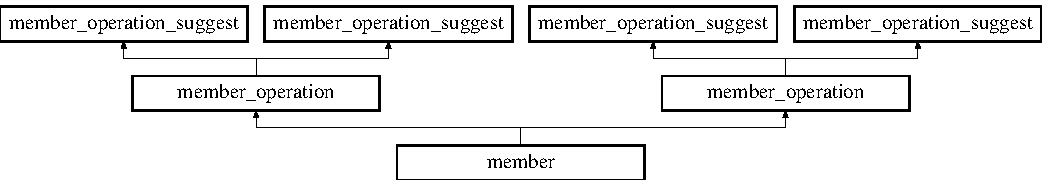
\includegraphics[height=2.413793cm]{classmember}
\end{center}
\end{figure}
\subsection*{Public Member Functions}
\begin{DoxyCompactItemize}
\item 
\hyperlink{classmember_aa2427c65795ffbdc72d64e2e91640463}{\-\_\-\-\_\-construct} (\$memberid)
\item 
\hyperlink{classmember_a364bea0f1ea59b67e68293ae5da9f413}{ismale} ()
\item 
\hyperlink{classmember_af93337d3c08cad93fa43b5f30c0215b0}{isfemale} ()
\item 
\hyperlink{classmember_a551821d3d6d64bbf0c6c4c5d62b3366c}{get\-Father} ()
\item 
\hyperlink{classmember_a8c6d2d7c3ad62d4988000e0886d394b2}{get\-Mother} ()
\item 
\hyperlink{classmember_af0d9a69479f2b9c859acb90e97bad85c}{get\-\_\-sons} ()
\item 
\hyperlink{classmember_a024f7356f2279490775b6ae432d51010}{has\-\_\-sons} ()
\item 
\hyperlink{classmember_a45c3ed97d49c45ce716892b4b5e44bd2}{autofix} ()
\item 
\hypertarget{classmember_ae1a0a03869debcb7e7f58eaca72fb2ed}{{\bfseries autofix2} ()}\label{classmember_ae1a0a03869debcb7e7f58eaca72fb2ed}

\item 
\hyperlink{classmember_ae0f93137fb23a9f5ae9e6a287f6232dd}{set\-\_\-relationship} (\$relationship\-\_\-id)
\item 
\hyperlink{classmember_a541afd2c1c096f5810c0b889e33287ba}{related\-\_\-to} (\$related\-\_\-to)
\item 
\hyperlink{classmember_aeb52158abb66bf82955ab17670b11eec}{gender} ()
\item 
\hyperlink{classmember_a7eccf6c8f3bc1bc775502427de8aaf7c}{get} (\$property\-Name)
\item 
\hyperlink{classmember_aa4b22929c0f9688d36c4528b467013d0}{set} (\$property\-Name, \$value)
\item 
\hyperlink{classmember_ac330497056943c44df23963f6a4d1288}{spouse} ()
\item 
\hyperlink{classmember_a2af2011afe5c6ee0404e2f45b93daf11}{is\-Admin} ()
\item 
\hypertarget{classmember_ad691ab2a161f3ad4a5c86435d08e7407}{{\bfseries send\-Forgot\-Password} ()}\label{classmember_ad691ab2a161f3ad4a5c86435d08e7407}

\item 
\hypertarget{classmember_a1e2c7b73375ee37813a78285b170cb79}{{\bfseries change\-Password} (\$new\-Password)}\label{classmember_a1e2c7b73375ee37813a78285b170cb79}

\end{DoxyCompactItemize}
\subsection*{Additional Inherited Members}


\subsection{Detailed Description}
This class is used to manipulate user data

\begin{DoxyAuthor}{Author}
piyush 
\end{DoxyAuthor}


Definition at line 10 of file member.\-php.



\subsection{Constructor \& Destructor Documentation}
\hypertarget{classmember_aa2427c65795ffbdc72d64e2e91640463}{\index{member@{member}!\-\_\-\-\_\-construct@{\-\_\-\-\_\-construct}}
\index{\-\_\-\-\_\-construct@{\-\_\-\-\_\-construct}!member@{member}}
\subsubsection[{\-\_\-\-\_\-construct}]{\setlength{\rightskip}{0pt plus 5cm}member\-::\-\_\-\-\_\-construct (
\begin{DoxyParamCaption}
\item[{}]{\$memberid}
\end{DoxyParamCaption}
)}}\label{classmember_aa2427c65795ffbdc72d64e2e91640463}
The constructor of the class 
\begin{DoxyParams}[1]{Parameters}
integer & {\em \$memberid} & The I\-D of the member \\
\hline
\end{DoxyParams}
\begin{DoxyReturn}{Returns}
null 
\end{DoxyReturn}


Definition at line 17 of file member.\-php.


\begin{DoxyCode}
17                                            \{
18         parent::\_\_construct($memberid);
19         $this->\hyperlink{classmember__operation_aaae269a6cda847ad7aaffad933fe0ee6}{populate\_data}($memberid);
20         $this->\hyperlink{classmember_a45c3ed97d49c45ce716892b4b5e44bd2}{autofix}();
21     \}
\end{DoxyCode}


\subsection{Member Function Documentation}
\hypertarget{classmember_a45c3ed97d49c45ce716892b4b5e44bd2}{\index{member@{member}!autofix@{autofix}}
\index{autofix@{autofix}!member@{member}}
\subsubsection[{autofix}]{\setlength{\rightskip}{0pt plus 5cm}member\-::autofix (
\begin{DoxyParamCaption}
{}
\end{DoxyParamCaption}
)}}\label{classmember_a45c3ed97d49c45ce716892b4b5e44bd2}
This function is used to fix any anamolies found in member data such as if user has children but the relationshipstatus is set to Single   \$db \begin{DoxyReturn}{Returns}
null 
\end{DoxyReturn}


Definition at line 102 of file member.\-php.


\begin{DoxyCode}
102                        \{
103 
104         $nosons = $this->\hyperlink{classmember_a024f7356f2279490775b6ae432d51010}{has\_sons}();
105         \textcolor{keywordflow}{if} ($nosons > 0) \{
106 \textcolor{comment}{// If the member has sons Change the status to married}
107 \textcolor{comment}{// Add a wife and add parents to wife and create a new family}
108             $this->\hyperlink{classmember_ae0f93137fb23a9f5ae9e6a287f6232dd}{set\_relationship}(MARRIED);
109             $this->\hyperlink{classmember__operation_a98d050cd93cb97b426d8971a827159b1}{addwife}();
110 
111 \textcolor{comment}{//Call the second autofix function to fix the wife and }
112 \textcolor{comment}{//husband of same family issue.}
113             $this->autofix2();
114         \}
115     \}
\end{DoxyCode}
\hypertarget{classmember_aeb52158abb66bf82955ab17670b11eec}{\index{member@{member}!gender@{gender}}
\index{gender@{gender}!member@{member}}
\subsubsection[{gender}]{\setlength{\rightskip}{0pt plus 5cm}member\-::gender (
\begin{DoxyParamCaption}
{}
\end{DoxyParamCaption}
)}}\label{classmember_aeb52158abb66bf82955ab17670b11eec}
Return the gender code of the member 1 = Female 0= Male \begin{DoxyReturn}{Returns}
integer 
\end{DoxyReturn}


Definition at line 186 of file member.\-php.


\begin{DoxyCode}
186                       \{
187         \textcolor{keywordflow}{return} $this->data[\textcolor{stringliteral}{'gender'}];
188     \}
\end{DoxyCode}
\hypertarget{classmember_a7eccf6c8f3bc1bc775502427de8aaf7c}{\index{member@{member}!get@{get}}
\index{get@{get}!member@{member}}
\subsubsection[{get}]{\setlength{\rightskip}{0pt plus 5cm}member\-::get (
\begin{DoxyParamCaption}
\item[{}]{\$property\-Name}
\end{DoxyParamCaption}
)}}\label{classmember_a7eccf6c8f3bc1bc775502427de8aaf7c}
\$db 
\begin{DoxyParams}[1]{Parameters}
type & {\em \$property\-Name} & \\
\hline
\end{DoxyParams}
\begin{DoxyReturn}{Returns}
type 
\end{DoxyReturn}


Definition at line 196 of file member.\-php.


\begin{DoxyCode}
196                                 \{
197         \textcolor{keywordflow}{return} $this->data[$propertyName];
198     \}
\end{DoxyCode}
\hypertarget{classmember_af0d9a69479f2b9c859acb90e97bad85c}{\index{member@{member}!get\-\_\-sons@{get\-\_\-sons}}
\index{get\-\_\-sons@{get\-\_\-sons}!member@{member}}
\subsubsection[{get\-\_\-sons}]{\setlength{\rightskip}{0pt plus 5cm}member\-::get\-\_\-sons (
\begin{DoxyParamCaption}
{}
\end{DoxyParamCaption}
)}}\label{classmember_af0d9a69479f2b9c859acb90e97bad85c}
This function is used to get the children of the currenyl logged-\/in user   \$db The instance of the db class \begin{DoxyReturn}{Returns}
array Array of  
\end{DoxyReturn}


Definition at line 73 of file member.\-php.


\begin{DoxyCode}
73                         \{
74         global $db;
75         $finalarray = array();
76         $query = $db->query(\textcolor{stringliteral}{"select * from member where sonof=$this->id"});
77         \textcolor{keywordflow}{while} ($row = $db->fetch($query)) \{
78             array\_push($finalarray, \textcolor{keyword}{new} \hyperlink{classmember}{member}($row[\textcolor{stringliteral}{'id'}]));
79         \}
80         \textcolor{keywordflow}{return} $finalarray;
81     \}
\end{DoxyCode}
\hypertarget{classmember_a551821d3d6d64bbf0c6c4c5d62b3366c}{\index{member@{member}!get\-Father@{get\-Father}}
\index{get\-Father@{get\-Father}!member@{member}}
\subsubsection[{get\-Father}]{\setlength{\rightskip}{0pt plus 5cm}member\-::get\-Father (
\begin{DoxyParamCaption}
{}
\end{DoxyParamCaption}
)}}\label{classmember_a551821d3d6d64bbf0c6c4c5d62b3366c}
This function is used to get the I\-D of the parent of the current logged in user \begin{DoxyReturn}{Returns}

\end{DoxyReturn}


Definition at line 52 of file member.\-php.


\begin{DoxyCode}
52                          \{
53         \textcolor{keywordflow}{return} \textcolor{keyword}{new} \hyperlink{classmember}{member}($this->data[\textcolor{stringliteral}{'sonof'}]);
54     \}
\end{DoxyCode}
\hypertarget{classmember_a8c6d2d7c3ad62d4988000e0886d394b2}{\index{member@{member}!get\-Mother@{get\-Mother}}
\index{get\-Mother@{get\-Mother}!member@{member}}
\subsubsection[{get\-Mother}]{\setlength{\rightskip}{0pt plus 5cm}member\-::get\-Mother (
\begin{DoxyParamCaption}
{}
\end{DoxyParamCaption}
)}}\label{classmember_a8c6d2d7c3ad62d4988000e0886d394b2}
\$db \begin{DoxyReturn}{Returns}

\end{DoxyReturn}


Definition at line 61 of file member.\-php.


\begin{DoxyCode}
61                          \{
62         global $db;
63         $query = $db->get(\textcolor{stringliteral}{"select related\_to from member where id = "} . $this->data[\textcolor{stringliteral}{'sonof'}]);
64 
65         \textcolor{keywordflow}{return} \textcolor{keyword}{new} \hyperlink{classmember}{member}($query[\textcolor{stringliteral}{'related\_to'}]);
66     \}
\end{DoxyCode}
\hypertarget{classmember_a024f7356f2279490775b6ae432d51010}{\index{member@{member}!has\-\_\-sons@{has\-\_\-sons}}
\index{has\-\_\-sons@{has\-\_\-sons}!member@{member}}
\subsubsection[{has\-\_\-sons}]{\setlength{\rightskip}{0pt plus 5cm}member\-::has\-\_\-sons (
\begin{DoxyParamCaption}
{}
\end{DoxyParamCaption}
)}}\label{classmember_a024f7356f2279490775b6ae432d51010}
This function is used to check if the user has children This function also return the number of children of the user   \$db The instance of the  class \begin{DoxyReturn}{Returns}
integer 
\end{DoxyReturn}


Definition at line 89 of file member.\-php.


\begin{DoxyCode}
89                         \{
90         global $db;
91         $query = $db->query(\textcolor{stringliteral}{"select count(*) as nosons from member where sonof=$this->id"});
92         $row = $db->fetch($query);
93         \textcolor{keywordflow}{return} $row[\textcolor{stringliteral}{'nosons'}];
94     \}
\end{DoxyCode}
\hypertarget{classmember_a2af2011afe5c6ee0404e2f45b93daf11}{\index{member@{member}!is\-Admin@{is\-Admin}}
\index{is\-Admin@{is\-Admin}!member@{member}}
\subsubsection[{is\-Admin}]{\setlength{\rightskip}{0pt plus 5cm}member\-::is\-Admin (
\begin{DoxyParamCaption}
{}
\end{DoxyParamCaption}
)}}\label{classmember_a2af2011afe5c6ee0404e2f45b93daf11}
\begin{DoxyReturn}{Returns}
boolean 
\end{DoxyReturn}


Definition at line 231 of file member.\-php.


\begin{DoxyCode}
231                        \{
232         \textcolor{keywordflow}{return} $this->data[\textcolor{stringliteral}{'admin'}];
233     \}
\end{DoxyCode}
\hypertarget{classmember_af93337d3c08cad93fa43b5f30c0215b0}{\index{member@{member}!isfemale@{isfemale}}
\index{isfemale@{isfemale}!member@{member}}
\subsubsection[{isfemale}]{\setlength{\rightskip}{0pt plus 5cm}member\-::isfemale (
\begin{DoxyParamCaption}
{}
\end{DoxyParamCaption}
)}}\label{classmember_af93337d3c08cad93fa43b5f30c0215b0}
Returns true if the user is female \begin{DoxyReturn}{Returns}
boolean 
\end{DoxyReturn}


Definition at line 39 of file member.\-php.


\begin{DoxyCode}
39                         \{
40         \textcolor{keywordflow}{if} ($this->data[\textcolor{stringliteral}{'gender'}] == FEMALE) \{
41             \textcolor{keywordflow}{return} \textcolor{keyword}{true};
42         \} \textcolor{keywordflow}{else} \{
43             \textcolor{keywordflow}{return} \textcolor{keyword}{false};
44         \}
45     \}
\end{DoxyCode}
\hypertarget{classmember_a364bea0f1ea59b67e68293ae5da9f413}{\index{member@{member}!ismale@{ismale}}
\index{ismale@{ismale}!member@{member}}
\subsubsection[{ismale}]{\setlength{\rightskip}{0pt plus 5cm}member\-::ismale (
\begin{DoxyParamCaption}
{}
\end{DoxyParamCaption}
)}}\label{classmember_a364bea0f1ea59b67e68293ae5da9f413}
Return true if the user is male \begin{DoxyReturn}{Returns}
boolean 
\end{DoxyReturn}


Definition at line 27 of file member.\-php.


\begin{DoxyCode}
27                       \{
28         \textcolor{keywordflow}{if} ($this->data[\textcolor{stringliteral}{'gender'}] == MALE) \{
29             \textcolor{keywordflow}{return} TRUE;
30         \} \textcolor{keywordflow}{else} \{
31             \textcolor{keywordflow}{return} \textcolor{keyword}{false};
32         \}
33     \}
\end{DoxyCode}
\hypertarget{classmember_a541afd2c1c096f5810c0b889e33287ba}{\index{member@{member}!related\-\_\-to@{related\-\_\-to}}
\index{related\-\_\-to@{related\-\_\-to}!member@{member}}
\subsubsection[{related\-\_\-to}]{\setlength{\rightskip}{0pt plus 5cm}member\-::related\-\_\-to (
\begin{DoxyParamCaption}
\item[{}]{\$related\-\_\-to}
\end{DoxyParamCaption}
)}}\label{classmember_a541afd2c1c096f5810c0b889e33287ba}
This function is add wife of the member. Returns true if successful else false. The member to be added as wife should already be created   \$db The instance of the db class 
\begin{DoxyParams}[1]{Parameters}
integer & {\em \$related\-\_\-to} & The I\-D of the member to be added as wife \\
\hline
\end{DoxyParams}
\begin{DoxyReturn}{Returns}
boolean 
\end{DoxyReturn}


Definition at line 169 of file member.\-php.


\begin{DoxyCode}
169                                      \{
170         global $db;
171         \textcolor{keywordflow}{if} ($db->query(\textcolor{stringliteral}{"update member set related\_to=$related\_to where id="} . $this->data[\textcolor{stringliteral}{'id'}])) \{
172             $this->\hyperlink{classmember_ae0f93137fb23a9f5ae9e6a287f6232dd}{set\_relationship}(MARRIED);
173 
174             \textcolor{keywordflow}{return} \textcolor{keyword}{true};
175         \} \textcolor{keywordflow}{else} \{
176             \textcolor{keywordflow}{return} \textcolor{keyword}{false};
177         \}
178     \}
\end{DoxyCode}
\hypertarget{classmember_aa4b22929c0f9688d36c4528b467013d0}{\index{member@{member}!set@{set}}
\index{set@{set}!member@{member}}
\subsubsection[{set}]{\setlength{\rightskip}{0pt plus 5cm}member\-::set (
\begin{DoxyParamCaption}
\item[{}]{\$property\-Name, }
\item[{}]{\$value}
\end{DoxyParamCaption}
)}}\label{classmember_aa4b22929c0f9688d36c4528b467013d0}
\$db 
\begin{DoxyParams}[1]{Parameters}
type & {\em \$property\-Name} & \\
\hline
type & {\em \$value} & \\
\hline
\end{DoxyParams}
\begin{DoxyReturn}{Returns}
type 
\end{DoxyReturn}


Definition at line 207 of file member.\-php.


\begin{DoxyCode}
207                                         \{
208         global $db;
209 
210         $query = $db->query(\textcolor{stringliteral}{"update member set $propertyName = '$value' where id = "} . $this->\textcolor{keywordtype}{id});
211 
212         \textcolor{keywordflow}{return} $query;
213     \}
\end{DoxyCode}
\hypertarget{classmember_ae0f93137fb23a9f5ae9e6a287f6232dd}{\index{member@{member}!set\-\_\-relationship@{set\-\_\-relationship}}
\index{set\-\_\-relationship@{set\-\_\-relationship}!member@{member}}
\subsubsection[{set\-\_\-relationship}]{\setlength{\rightskip}{0pt plus 5cm}member\-::set\-\_\-relationship (
\begin{DoxyParamCaption}
\item[{}]{\$relationship\-\_\-id}
\end{DoxyParamCaption}
)}}\label{classmember_ae0f93137fb23a9f5ae9e6a287f6232dd}
This function is used to set the relationship status of the current user Returns true if successfull else false   \$db The instance of the  class 
\begin{DoxyParams}[1]{Parameters}
integer & {\em \$relationship\-\_\-id} & The relationship I\-D. See Below. \\
\hline
\end{DoxyParams}
\begin{DoxyReturn}{Returns}
boolean
\end{DoxyReturn}
Relationship I\-D 0 == Single 1 == Married 

Definition at line 153 of file member.\-php.


\begin{DoxyCode}
153                                                 \{
154         global $db;
155         \textcolor{keywordflow}{if} (!$db->query(\textcolor{stringliteral}{"update member set relationship\_status=$relationship\_id where id=$this->id"})) \{
156             \textcolor{keywordflow}{return} \textcolor{keyword}{false};
157         \} \textcolor{keywordflow}{else} \{
158             \textcolor{keywordflow}{return} \textcolor{keyword}{true};
159         \}
160     \}
\end{DoxyCode}
\hypertarget{classmember_ac330497056943c44df23963f6a4d1288}{\index{member@{member}!spouse@{spouse}}
\index{spouse@{spouse}!member@{member}}
\subsubsection[{spouse}]{\setlength{\rightskip}{0pt plus 5cm}member\-::spouse (
\begin{DoxyParamCaption}
{}
\end{DoxyParamCaption}
)}}\label{classmember_ac330497056943c44df23963f6a4d1288}
\begin{DoxyReturn}{Returns}
boolean$\vert$ 
\end{DoxyReturn}


Definition at line 219 of file member.\-php.


\begin{DoxyCode}
219                       \{
220         \textcolor{keywordflow}{if} ($this->data[\textcolor{stringliteral}{'relationship\_status'}] == MARRIED) \{
221             \textcolor{keywordflow}{return} \textcolor{keyword}{new} \hyperlink{classmember}{member}($this->data[\textcolor{stringliteral}{'related\_to'}]);
222         \} \textcolor{keywordflow}{else} \{
223             \textcolor{keywordflow}{return} \textcolor{keyword}{false};
224         \}
225     \}
\end{DoxyCode}


The documentation for this class was generated from the following file\-:\begin{DoxyCompactItemize}
\item 
vanshavali/member.\-php\end{DoxyCompactItemize}

\hypertarget{classmember__operation}{\section{member\-\_\-operation Class Reference}
\label{classmember__operation}\index{member\-\_\-operation@{member\-\_\-operation}}
}
Inheritance diagram for member\-\_\-operation\-:\begin{figure}[H]
\begin{center}
\leavevmode
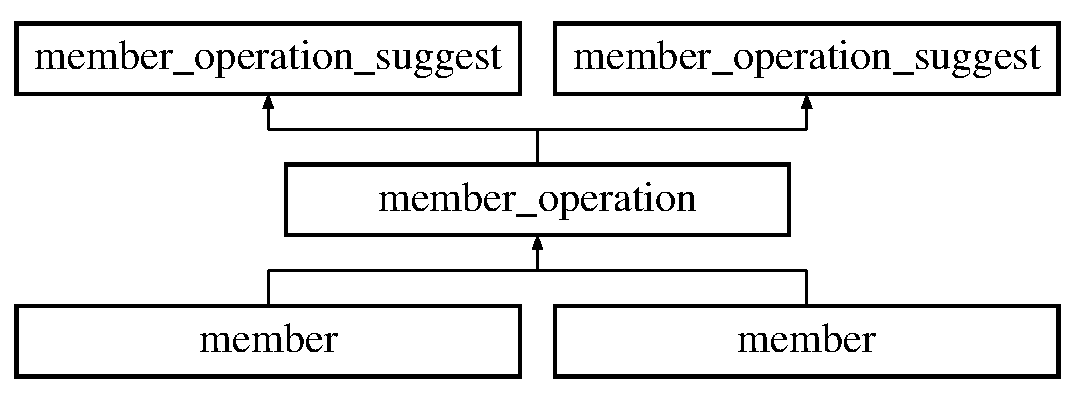
\includegraphics[height=3.000000cm]{classmember__operation}
\end{center}
\end{figure}
\subsection*{Public Member Functions}
\begin{DoxyCompactItemize}
\item 
\hyperlink{classmember__operation_a6878b5586bd9ea7e86c0ec19750437ca}{\-\_\-\-\_\-construct} (\$memberid)
\item 
\hyperlink{classmember__operation_aaae269a6cda847ad7aaffad933fe0ee6}{populate\-\_\-data} (\$memberid)
\item 
\hyperlink{classmember__operation_a6262e1076fe11fe6c0ef4311bfb79ac7}{add\-\_\-son} (\$name, \$gender, \$\hyperlink{classsuggest}{suggest}=false)
\item 
\hyperlink{classmember__operation_ad769e90d19b213f2d74966d5c1ea2af3}{hasspouse} ()
\item 
\hyperlink{classmember__operation_a98d050cd93cb97b426d8971a827159b1}{addwife} (\$name=\char`\"{}Wife\char`\"{}, \$suggest=false)
\item 
\hyperlink{classmember__operation_adc35cdeaaa4979bf5b8d602dd4f2b529}{addhusband} (\$name=\char`\"{}Husband\char`\"{}, \$suggest=false)
\item 
\hyperlink{classmember__operation_ac684b0752ce7aeafd21aab1aed081711}{remove} (\$\hyperlink{classsuggest}{suggest}=false)
\item 
\hyperlink{classmember__operation_ada4a29c07083c0b2986e5960ef223bed}{edit} (\$name, \$gender, \$relationship, \$dob, \$alive, \$\hyperlink{classsuggest}{suggest}=F\-A\-L\-S\-E)
\end{DoxyCompactItemize}
\subsection*{Public Attributes}
\begin{DoxyCompactItemize}
\item 
\hypertarget{classmember__operation_a734eb4b1794b8d73016ab6e47fef1b7c}{{\bfseries \$id}}\label{classmember__operation_a734eb4b1794b8d73016ab6e47fef1b7c}

\item 
\hypertarget{classmember__operation_aca6848da2c5d1928b415345ab7a1492b}{{\bfseries \$data}}\label{classmember__operation_aca6848da2c5d1928b415345ab7a1492b}

\end{DoxyCompactItemize}


\subsection{Detailed Description}
This class handles Member Entity To be Only used by other classes

\begin{DoxyAuthor}{Author}
piyush 
\end{DoxyAuthor}


Definition at line 11 of file member\-\_\-operation.\-php.



\subsection{Constructor \& Destructor Documentation}
\hypertarget{classmember__operation_a6878b5586bd9ea7e86c0ec19750437ca}{\index{member\-\_\-operation@{member\-\_\-operation}!\-\_\-\-\_\-construct@{\-\_\-\-\_\-construct}}
\index{\-\_\-\-\_\-construct@{\-\_\-\-\_\-construct}!member_operation@{member\-\_\-operation}}
\subsubsection[{\-\_\-\-\_\-construct}]{\setlength{\rightskip}{0pt plus 5cm}member\-\_\-operation\-::\-\_\-\-\_\-construct (
\begin{DoxyParamCaption}
\item[{}]{\$memberid}
\end{DoxyParamCaption}
)}}\label{classmember__operation_a6878b5586bd9ea7e86c0ec19750437ca}
Constructor of the class 
\begin{DoxyParams}[1]{Parameters}
integer & {\em \$memberid} & The I\-D of the member \\
\hline
\end{DoxyParams}
\begin{DoxyReturn}{Returns}
null 
\end{DoxyReturn}


Definition at line 30 of file member\-\_\-operation.\-php.


\begin{DoxyCode}
30                                            \{
31         $this->\textcolor{keywordtype}{id} = $memberid;
32     \}
\end{DoxyCode}


\subsection{Member Function Documentation}
\hypertarget{classmember__operation_a6262e1076fe11fe6c0ef4311bfb79ac7}{\index{member\-\_\-operation@{member\-\_\-operation}!add\-\_\-son@{add\-\_\-son}}
\index{add\-\_\-son@{add\-\_\-son}!member_operation@{member\-\_\-operation}}
\subsubsection[{add\-\_\-son}]{\setlength{\rightskip}{0pt plus 5cm}member\-\_\-operation\-::add\-\_\-son (
\begin{DoxyParamCaption}
\item[{}]{\$name, }
\item[{}]{\$gender, }
\item[{}]{\$suggest = {\ttfamily false}}
\end{DoxyParamCaption}
)}}\label{classmember__operation_a6262e1076fe11fe6c0ef4311bfb79ac7}
\-: Change name of the function. Misleading it is as it also works for daughters.

This function is used to add a child of the member. Returns false on error   \$db The instance of db class 
\begin{DoxyParams}[1]{Parameters}
string & {\em \$name} & The name of the new member \\
\hline
integer & {\em \$gender} & The gender of the new member \\
\hline
boolean & {\em \$suggest} & If this is a suggestion then set this to true \\
\hline
\end{DoxyParams}
\begin{DoxyReturn}{Returns}
integer The I\-D of the new member just added 
\end{DoxyReturn}


Definition at line 61 of file member\-\_\-operation.\-php.


\begin{DoxyCode}
61                                                        \{
62         global $vanshavali, $user;
63 
64         \textcolor{comment}{//Check for member to member access}
65         $hasAccess = $vanshavali->hasAccess($user->user[\textcolor{stringliteral}{'id'}], $this->id);
66 
67         \textcolor{keywordflow}{if} ($suggest & !$hasAccess) \{
68             \textcolor{keywordflow}{if} (intval($this->data[\textcolor{stringliteral}{'gender'}]) == MALE) \{
69 
70                 \textcolor{comment}{//If a male member then send his id}
71                 \textcolor{keywordflow}{return} parent::add\_son\_suggest($name, $gender, $this->data[\textcolor{stringliteral}{'id'}]);
72             \} \textcolor{keywordflow}{else} \{
73 
74                 \textcolor{comment}{//If not a male member then send the id of the spouse}
75                 \textcolor{keywordflow}{return} parent::add\_son\_suggest($name, $gender, $this->data[\textcolor{stringliteral}{'related\_to'}]);
76             \}
77         \} \textcolor{keywordflow}{else} \{
78 
79             \textcolor{comment}{//Before doing all this check if the member has a wife}
80             \textcolor{keywordflow}{if} ($this->\hyperlink{classmember__operation_ad769e90d19b213f2d74966d5c1ea2af3}{hasspouse}()) \{
81 
82                 \textcolor{comment}{//Add son directly to the Member database}
83                 global $db;
84 
85                 \textcolor{comment}{//Get the familyid of the parent}
86 
87                 \textcolor{comment}{/* @var $familyid integer */}
88                 $familyid = $this->data[\textcolor{stringliteral}{'family\_id'}];
89                 \textcolor{keywordflow}{if} (empty($familyid)) \{
90 
91                     \textcolor{comment}{//If family id is not defined than assume that he/she belongs to the default family}
92                     trigger\_error(\textcolor{stringliteral}{"Empty Family. Don't belong to any Family"}, E\_USER\_ERROR);
93                 \}
94 
95 
96                 \textcolor{comment}{//Prepare the sql according to the gender}
97                 $sql = \textcolor{stringliteral}{""};
98                 \textcolor{keywordflow}{if} (intval($this->data[\textcolor{stringliteral}{'gender'}]) === FEMALE) \{
99                     $sql = \textcolor{stringliteral}{"Insert into member(membername,gender,sonof,family\_id) }
100 \textcolor{stringliteral}{                values('$name',$gender,"} . $this->data[\textcolor{stringliteral}{'related\_to'}] . \textcolor{stringliteral}{",$familyid)"};
101                 \} \textcolor{keywordflow}{else} \{
102                     $sql = \textcolor{stringliteral}{"Insert into member(membername,gender,sonof,family\_id) }
103 \textcolor{stringliteral}{                values('$name',$gender,"} . $this->data[\textcolor{stringliteral}{'id'}] . \textcolor{stringliteral}{",$familyid)"};
104                 \}
105 
106                 \textcolor{comment}{//Execute the sql}
107                 \textcolor{keywordflow}{if} (!$db->get($sql)) \{
108                     trigger\_error(\textcolor{stringliteral}{"Cannot add member. Error executing the query"});
109                     \textcolor{keywordflow}{return} \textcolor{keyword}{false};
110                 \}
111                 \textcolor{keywordflow}{return} mysql\_insert\_id();
112             \} \textcolor{keywordflow}{else} \{
113                 \textcolor{keywordflow}{return} \textcolor{keyword}{false};
114             \}
115         \}
116     \}
\end{DoxyCode}
\hypertarget{classmember__operation_adc35cdeaaa4979bf5b8d602dd4f2b529}{\index{member\-\_\-operation@{member\-\_\-operation}!addhusband@{addhusband}}
\index{addhusband@{addhusband}!member_operation@{member\-\_\-operation}}
\subsubsection[{addhusband}]{\setlength{\rightskip}{0pt plus 5cm}member\-\_\-operation\-::addhusband (
\begin{DoxyParamCaption}
\item[{}]{\$name = {\ttfamily \char`\"{}Husband\char`\"{}}, }
\item[{}]{\$suggest = {\ttfamily false}}
\end{DoxyParamCaption}
)}}\label{classmember__operation_adc35cdeaaa4979bf5b8d602dd4f2b529}
This function is used to add husband to the member. It returns true on successfull operation.   \$vanshavali Instance of the  class   \$db Instance of the  class 
\begin{DoxyParams}[1]{Parameters}
string & {\em \$name} & The name of the husband \\
\hline
boolean & {\em \$suggest} & Set to true if is a suggestion \\
\hline
\end{DoxyParams}
\begin{DoxyReturn}{Returns}
boolean 
\end{DoxyReturn}


Definition at line 190 of file member\-\_\-operation.\-php.


\begin{DoxyCode}
190                                                              \{
191         global $vanshavali, $user;
192 
193         $hasAccess = $vanshavali->hasAccess($user->user[\textcolor{stringliteral}{'id'}], $this->id);
194 
195         \textcolor{keywordflow}{if} ($suggest && !$hasAccess) \{
196             \textcolor{keywordflow}{return} parent::addhusband\_suggest($name, $this->\textcolor{keywordtype}{id});
197         \} \textcolor{keywordflow}{else} \{
198 
199             \textcolor{comment}{//Add wife directly in the database}
200             $family\_id = $vanshavali->addfamily($name . \textcolor{stringliteral}{"'s Family"});
201             \textcolor{keywordflow}{if} ($family\_id) \{
202                 \textcolor{comment}{// Now add parents with that family id}
203                 $fatherid = $vanshavali->addmember\_explicit(\textcolor{stringliteral}{"Father"}, 0, $family\_id);
204                 $motherid = $vanshavali->addmember\_explicit(\textcolor{stringliteral}{"Mother"}, 1, $family\_id);
205 
206                 $father = $vanshavali->getmember($fatherid);
207                 $mother = $vanshavali->getmember($motherid);
208 
209                 $mother->related\_to($fatherid);
210                 $father->related\_to($motherid);
211 
212                 $wife = \textcolor{keyword}{new} \hyperlink{classmember}{member}($father->add\_son(\textcolor{stringliteral}{"Wife"}, 0));
213                 $this->related\_to($wife->id);
214                 $this->set\_relationship(1);
215                 $wife->related\_to($this->\textcolor{keywordtype}{id});
216                 $wife->set\_relationship(1);
217                 \textcolor{keywordflow}{return} \textcolor{keyword}{true};
218             \} \textcolor{keywordflow}{else} \{
219                 \textcolor{keywordflow}{return} \textcolor{keyword}{false};
220             \}
221         \}
222     \}
\end{DoxyCode}
\hypertarget{classmember__operation_a98d050cd93cb97b426d8971a827159b1}{\index{member\-\_\-operation@{member\-\_\-operation}!addwife@{addwife}}
\index{addwife@{addwife}!member_operation@{member\-\_\-operation}}
\subsubsection[{addwife}]{\setlength{\rightskip}{0pt plus 5cm}member\-\_\-operation\-::addwife (
\begin{DoxyParamCaption}
\item[{}]{\$name = {\ttfamily \char`\"{}Wife\char`\"{}}, }
\item[{}]{\$suggest = {\ttfamily false}}
\end{DoxyParamCaption}
)}}\label{classmember__operation_a98d050cd93cb97b426d8971a827159b1}
This function is used to add wife to the member. Returns true if successfull operation else returns false   \$vanshavali The instance of the  class   \$db The instance of the  class 
\begin{DoxyParams}[1]{Parameters}
string & {\em \$name} & The name of Wife \\
\hline
boolean & {\em \$suggest} & Set to true if this is a suggestion \\
\hline
\end{DoxyParams}
\begin{DoxyReturn}{Returns}
boolean 
\end{DoxyReturn}


Definition at line 145 of file member\-\_\-operation.\-php.


\begin{DoxyCode}
145                                                        \{
146         global $vanshavali, $user;
147 
148         \textcolor{keywordflow}{if} ($suggest && !$hasAccess) \{
149             \textcolor{keywordflow}{return} parent::addwife\_suggest($name, $this->\textcolor{keywordtype}{id});
150         \} \textcolor{keywordflow}{else} \{
151 
152             \textcolor{comment}{//Firstly to check if the member already has a wife}
153             \textcolor{keywordflow}{if} (!$this->\hyperlink{classmember__operation_ad769e90d19b213f2d74966d5c1ea2af3}{hasspouse}()) \{
154                 \textcolor{comment}{//Add wife directly in the database}
155                 $father\_family\_id = $vanshavali->addfamily($name);
156                 $mother\_family\_id = $vanshavali->addfamily($name);
157                 \textcolor{keywordflow}{if} ($father\_family\_id && $mother\_family\_id) \{
158                     \textcolor{comment}{// Now add parents with that family id}
159                     $fatherid = $vanshavali->addmember\_explicit(\textcolor{stringliteral}{"Father"}, MALE, $father\_family\_id);
160                     $motherid = $vanshavali->addmember\_explicit(\textcolor{stringliteral}{"Mother"}, FEMALE, $mother\_family\_id);
161 
162                     $father = $vanshavali->getmember($fatherid);
163                     $mother = $vanshavali->getmember($motherid);
164 
165                     $mother->related\_to($fatherid);
166                     $father->related\_to($motherid);
167 
168                     $wife = \textcolor{keyword}{new} \hyperlink{classmember}{member}($father->add\_son(\textcolor{stringliteral}{"Wife"}, FEMALE));
169                     $this->related\_to($wife->id);
170                     $this->set\_relationship(MARRIED);
171                     $wife->related\_to($this->\textcolor{keywordtype}{id});
172                     $wife->set\_relationship(MARRIED);
173                     \textcolor{keywordflow}{return} \textcolor{keyword}{true};
174                 \} \textcolor{keywordflow}{else} \{
175                     \textcolor{keywordflow}{return} \textcolor{keyword}{false};
176                 \}
177             \}
178         \}
179     \}
\end{DoxyCode}
\hypertarget{classmember__operation_ada4a29c07083c0b2986e5960ef223bed}{\index{member\-\_\-operation@{member\-\_\-operation}!edit@{edit}}
\index{edit@{edit}!member_operation@{member\-\_\-operation}}
\subsubsection[{edit}]{\setlength{\rightskip}{0pt plus 5cm}member\-\_\-operation\-::edit (
\begin{DoxyParamCaption}
\item[{}]{\$name, }
\item[{}]{\$gender, }
\item[{}]{\$relationship, }
\item[{}]{\$dob, }
\item[{}]{\$alive, }
\item[{}]{\$suggest = {\ttfamily FALSE}}
\end{DoxyParamCaption}
)}}\label{classmember__operation_ada4a29c07083c0b2986e5960ef223bed}
This function is used to edit a user details. Returns true on successful operation else returns false   \$db 
\begin{DoxyParams}[1]{Parameters}
string & {\em \$name} & The new name of the member \\
\hline
integer & {\em \$gender} & The new gender of the member. See Below. \\
\hline
integer & {\em \$relationship} & The relationship status of the member See Below. \\
\hline
integer & {\em \$dob} & The Timestamp of the D\-O\-B of the member \\
\hline
Integer & {\em \$alive} & The living status of the member \\
\hline
boolean & {\em \$suggest} & Set to true if this is a suggest \\
\hline
\end{DoxyParams}
\begin{DoxyReturn}{Returns}
boolean
\end{DoxyReturn}
Gender 0 == Male 1 == Female

Relationship Status 0 == Single 1 == Married

Alive 0 == Deceased 1 == Living 

Definition at line 277 of file member\-\_\-operation.\-php.


\begin{DoxyCode}
277                                                                                  \{
278         global $vanshavali, $user;
279 
280         $hasAccess = $vanshavali->hasAccess($user->user[\textcolor{stringliteral}{'id'}], $this->id);
281 
282         \textcolor{keywordflow}{if} ($suggest && !$hasAccess) \{
283             \textcolor{keywordflow}{return} parent::edit\_suggest($name, $gender, $relationship, $dob, $alive, $this->data[\textcolor{stringliteral}{'id'}]);
284         \} \textcolor{keywordflow}{else} \{
285             \textcolor{comment}{//Change the details directly...}
286             global $db;
287 
288             \textcolor{comment}{//Prepare the sql and execute it...}
289             \textcolor{keywordflow}{if} (!$db->get(\textcolor{stringliteral}{"Update member set membername='$name',gender=$gender,}
290 \textcolor{stringliteral}{                relationship\_status=$relationship,dob=$dob, alive=$alive where id="} . $this->data[\textcolor{stringliteral}{'id'}])) \{
291                 trigger\_error(\textcolor{stringliteral}{"Error Editing member. Error Executing query"});
292                 \textcolor{keywordflow}{return} FALSE;
293             \}
294         \}
295 
296         \textcolor{comment}{//If reached till here, then the operation is complete}
297         \textcolor{keywordflow}{return} True;
298     \}
\end{DoxyCode}
\hypertarget{classmember__operation_ad769e90d19b213f2d74966d5c1ea2af3}{\index{member\-\_\-operation@{member\-\_\-operation}!hasspouse@{hasspouse}}
\index{hasspouse@{hasspouse}!member_operation@{member\-\_\-operation}}
\subsubsection[{hasspouse}]{\setlength{\rightskip}{0pt plus 5cm}member\-\_\-operation\-::hasspouse (
\begin{DoxyParamCaption}
{}
\end{DoxyParamCaption}
)}}\label{classmember__operation_ad769e90d19b213f2d74966d5c1ea2af3}
This function is used to check if check if the member has a spouse or not Returns true If the member has spouse else returns false   \$db The instance of the db class \begin{DoxyReturn}{Returns}
boolean 
\end{DoxyReturn}


Definition at line 124 of file member\-\_\-operation.\-php.


\begin{DoxyCode}
124                          \{
125         global $db;
126 
127         $row = $db->get(\textcolor{stringliteral}{"select related\_to from member where id="} . $this->\textcolor{keywordtype}{id});
128 
129         \textcolor{keywordflow}{if} (!empty($row[\textcolor{stringliteral}{'related\_to'}])) \{
130             \textcolor{keywordflow}{return} \textcolor{keyword}{true};
131         \} \textcolor{keywordflow}{else} \{
132             \textcolor{keywordflow}{return} \textcolor{keyword}{false};
133         \}
134     \}
\end{DoxyCode}
\hypertarget{classmember__operation_aaae269a6cda847ad7aaffad933fe0ee6}{\index{member\-\_\-operation@{member\-\_\-operation}!populate\-\_\-data@{populate\-\_\-data}}
\index{populate\-\_\-data@{populate\-\_\-data}!member_operation@{member\-\_\-operation}}
\subsubsection[{populate\-\_\-data}]{\setlength{\rightskip}{0pt plus 5cm}member\-\_\-operation\-::populate\-\_\-data (
\begin{DoxyParamCaption}
\item[{}]{\$memberid}
\end{DoxyParamCaption}
)}}\label{classmember__operation_aaae269a6cda847ad7aaffad933fe0ee6}
This function is used to fill the \$data variable with member data   \$db The instance of the  class 
\begin{DoxyParams}[1]{Parameters}
integer & {\em \$memberid} & The I\-D of the member \\
\hline
\end{DoxyParams}
\begin{DoxyReturn}{Returns}
null 
\end{DoxyReturn}


Definition at line 40 of file member\-\_\-operation.\-php.


\begin{DoxyCode}
40                                       \{
41         \textcolor{comment}{// Fill user variable with user data}
42         global $db;
43         $query = $db->query(\textcolor{stringliteral}{"Select * from member where id=$memberid"});
44         $row = $db->fetch($query);
45         $this->data = $row;
46 
47         \textcolor{comment}{//Adding a check for the name. This is when user forgets to add name in the suggestion.}
48         $row[\textcolor{stringliteral}{'membername'}] = trim($row[\textcolor{stringliteral}{'membername'}]) == \textcolor{stringliteral}{""} ? \textcolor{stringliteral}{"unknown"} : $row[\textcolor{stringliteral}{'membername'}];
49     \}
\end{DoxyCode}
\hypertarget{classmember__operation_ac684b0752ce7aeafd21aab1aed081711}{\index{member\-\_\-operation@{member\-\_\-operation}!remove@{remove}}
\index{remove@{remove}!member_operation@{member\-\_\-operation}}
\subsubsection[{remove}]{\setlength{\rightskip}{0pt plus 5cm}member\-\_\-operation\-::remove (
\begin{DoxyParamCaption}
\item[{}]{\$suggest = {\ttfamily false}}
\end{DoxyParamCaption}
)}}\label{classmember__operation_ac684b0752ce7aeafd21aab1aed081711}
This function is used to remove the member from the database Returns true on successfull operation else false   \$db Instance of the  class 
\begin{DoxyParams}[1]{Parameters}
boolean & {\em \$suggest} & Set to true if is a suggestion \\
\hline
\end{DoxyParams}
\begin{DoxyReturn}{Returns}
boolean 
\end{DoxyReturn}


Definition at line 231 of file member\-\_\-operation.\-php.


\begin{DoxyCode}
231                                       \{
232 
233         global $vanshavali, $user;
234 
235         $hasAccess = $vanshavali->hasAccess($user->user[\textcolor{stringliteral}{'id'}], $this->id);
236         \textcolor{keywordflow}{if} ($suggest && !$hasAccess) \{
237             \textcolor{keywordflow}{return} parent::remove\_suggest($this->data[\textcolor{stringliteral}{'id'}]);
238         \} \textcolor{keywordflow}{else} \{
239             \textcolor{comment}{//Remove the member completely}
240             global $db;
241 
242             \textcolor{comment}{//Prepare the sql}
243             \textcolor{keywordflow}{if} (!$db->get(\textcolor{stringliteral}{"Update member set dontshow=1 where id="} . $this->data[\textcolor{stringliteral}{'id'}])) \{
244                 trigger\_error(\textcolor{stringliteral}{"Cannot delete member. Error Executing the query"});
245                 \textcolor{keywordflow}{return} \textcolor{keyword}{false};
246             \}
247         \}
248 
249         \textcolor{comment}{//If reached here, then the operations is complete}
250         \textcolor{keywordflow}{return} \textcolor{keyword}{true};
251     \}
\end{DoxyCode}


The documentation for this class was generated from the following file\-:\begin{DoxyCompactItemize}
\item 
vanshavali/member\-\_\-operation.\-php\end{DoxyCompactItemize}

\hypertarget{classmodule}{\section{module Class Reference}
\label{classmodule}\index{module@{module}}
}
\subsection*{Public Member Functions}
\begin{DoxyCompactItemize}
\item 
\hypertarget{classmodule_ab057dc4f65b592345dffb5de10e24027}{{\bfseries \-\_\-\-\_\-construct} (\$getarray, \$template, \$\hyperlink{classdb}{db})}\label{classmodule_ab057dc4f65b592345dffb5de10e24027}

\end{DoxyCompactItemize}
\subsection*{Protected Attributes}
\begin{DoxyCompactItemize}
\item 
\hypertarget{classmodule_af7b7b336d419f89e3eeb89c41eec77f8}{{\bfseries \$getvars}}\label{classmodule_af7b7b336d419f89e3eeb89c41eec77f8}

\item 
\hypertarget{classmodule_a9ebd6fe2f161764e0f9946999b10d33d}{{\bfseries \$template}}\label{classmodule_a9ebd6fe2f161764e0f9946999b10d33d}

\item 
\hypertarget{classmodule_a56afb8b18363105cd10edb7c74749e50}{{\bfseries \$db}}\label{classmodule_a56afb8b18363105cd10edb7c74749e50}

\end{DoxyCompactItemize}


\subsection{Detailed Description}
Description of module

\begin{DoxyAuthor}{Author}
piyush 
\end{DoxyAuthor}


Definition at line 8 of file module.\-php.



The documentation for this class was generated from the following file\-:\begin{DoxyCompactItemize}
\item 
admin/module.\-php\end{DoxyCompactItemize}

\hypertarget{classsuggest}{\section{suggest Class Reference}
\label{classsuggest}\index{suggest@{suggest}}
}
Inheritance diagram for suggest\-:\begin{figure}[H]
\begin{center}
\leavevmode
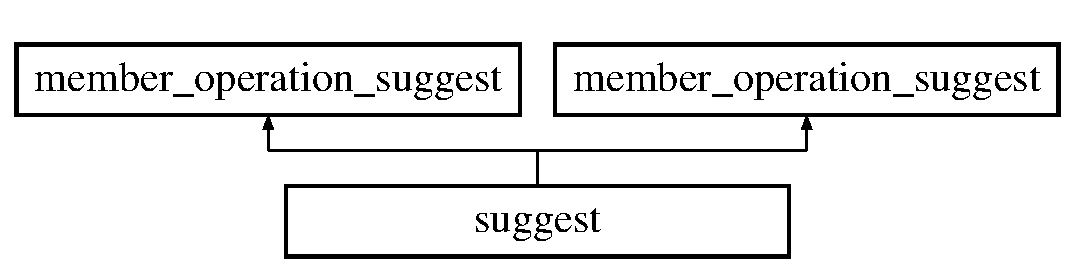
\includegraphics[height=2.000000cm]{classsuggest}
\end{center}
\end{figure}
\subsection*{Public Member Functions}
\begin{DoxyCompactItemize}
\item 
\hyperlink{classsuggest_a6e0521c192159953fda4bd293b01d440}{\-\_\-\-\_\-construct} (\$suggestid)
\item 
\hyperlink{classsuggest_a88a3a93bbc97e562d8f4a2b04bc72d14}{approve} ()
\item 
\hyperlink{classsuggest_a7786abfabcc1c14520f6199d1e93bbb2}{reject} ()
\item 
\hyperlink{classsuggest_aea8963c5a27e226cd1bbc039d14c39bd}{dontknow} ()
\item 
\hyperlink{classsuggest_aec18fc5fc3aa1f7ab553f632d822bd91}{checkpercent} ()
\item 
\hyperlink{classsuggest_a32f9238a6ea3e85021319f6cec2f6fca}{approval\-\_\-delete} ()
\end{DoxyCompactItemize}
\subsection*{Public Attributes}
\begin{DoxyCompactItemize}
\item 
\hypertarget{classsuggest_a803056257d5db2637c35becdc6f8ddc8}{{\bfseries \$id}}\label{classsuggest_a803056257d5db2637c35becdc6f8ddc8}

\item 
\hypertarget{classsuggest_afde8633e323581d390c204893b54a2f3}{{\bfseries \$suggested\-\_\-value}}\label{classsuggest_afde8633e323581d390c204893b54a2f3}

\item 
\hypertarget{classsuggest_a8e540fe8897c430a0e0fab8760036b40}{{\bfseries \$typesuggest}}\label{classsuggest_a8e540fe8897c430a0e0fab8760036b40}

\item 
\hypertarget{classsuggest_a013083c80765c478262f28166c8f1491}{{\bfseries \$suggestedby}}\label{classsuggest_a013083c80765c478262f28166c8f1491}

\end{DoxyCompactItemize}
\subsection*{Private Member Functions}
\begin{DoxyCompactItemize}
\item 
\hyperlink{classsuggest_a9ddef5aac5c98ef0d45e23ac8c802ee0}{check\-\_\-decision} ()
\item 
\hyperlink{classsuggest_aaa4dc18391cb837d8c7a5448992790e9}{apply} ()
\end{DoxyCompactItemize}


\subsection{Detailed Description}
Suggestion Class is used to add, remove or edit suggestions Basically a Class to operate on suggested\-\_\-info and suggest\-\_\-approval table

\begin{DoxyAuthor}{Author}
piyush 
\end{DoxyAuthor}


Definition at line 11 of file suggest.\-php.



\subsection{Constructor \& Destructor Documentation}
\hypertarget{classsuggest_a6e0521c192159953fda4bd293b01d440}{\index{suggest@{suggest}!\-\_\-\-\_\-construct@{\-\_\-\-\_\-construct}}
\index{\-\_\-\-\_\-construct@{\-\_\-\-\_\-construct}!suggest@{suggest}}
\subsubsection[{\-\_\-\-\_\-construct}]{\setlength{\rightskip}{0pt plus 5cm}suggest\-::\-\_\-\-\_\-construct (
\begin{DoxyParamCaption}
\item[{}]{\$suggestid}
\end{DoxyParamCaption}
)}}\label{classsuggest_a6e0521c192159953fda4bd293b01d440}
Constructor of the class. This gathers the basic information about the suggestion which is to be managed   \$db Instance of the db class 
\begin{DoxyParams}[1]{Parameters}
integer & {\em \$suggestid} & The I\-D of the suggestion to be managed \\
\hline
\end{DoxyParams}


Definition at line 21 of file suggest.\-php.


\begin{DoxyCode}
21                                      \{
22         global $db;
23         $this->\textcolor{keywordtype}{id} = $suggestid;
24         $row = $db->get(\textcolor{stringliteral}{"select * from suggested\_info where id=$suggestid"});
25         \textcolor{comment}{//$this->suggested\_value = json\_decode($row['suggested\_value'], TRUE);}
26         $this->typesuggest = $row[\textcolor{stringliteral}{'typesuggest'}];
27         $this->suggestedby = $row[\textcolor{stringliteral}{'suggested\_by'}];
28 
29         \textcolor{comment}{//if typesuggest is remove then suggested value is in json else not}
30         \textcolor{keywordflow}{if} (in\_array($row[\textcolor{stringliteral}{'typesuggest'}], array(DEL, ADD))) \{
31             $this->suggested\_value = $row[\textcolor{stringliteral}{'new\_value'}];
32         \} \textcolor{keywordflow}{else} \{
33             $this->suggested\_value = json\_decode($row[\textcolor{stringliteral}{'new\_value'}], \textcolor{keyword}{true});
34         \}
35     \}
\end{DoxyCode}


\subsection{Member Function Documentation}
\hypertarget{classsuggest_aaa4dc18391cb837d8c7a5448992790e9}{\index{suggest@{suggest}!apply@{apply}}
\index{apply@{apply}!suggest@{suggest}}
\subsubsection[{apply}]{\setlength{\rightskip}{0pt plus 5cm}suggest\-::apply (
\begin{DoxyParamCaption}
{}
\end{DoxyParamCaption}
)\hspace{0.3cm}{\ttfamily [private]}}}\label{classsuggest_aaa4dc18391cb837d8c7a5448992790e9}
This function is used to accept the suggestion and apply the changes to the main member table   \$vanshavali Instance of the vanshavali class   \$db Instance of the db class \begin{DoxyReturn}{Returns}
null 
\end{DoxyReturn}


Definition at line 168 of file suggest.\-php.


\begin{DoxyCode}
168                              \{
169         global $vanshavali, $db, $suggest\_handler;
170 
171         \textcolor{comment}{//Check if suggested\_value was JSON or not}
172         \textcolor{keywordflow}{if} (is\_array($this->suggested\_value)) \{
173             $member = $vanshavali->getmember($this->suggested\_value[\textcolor{stringliteral}{'id'}]);
174         \} \textcolor{keywordflow}{else} \{
175             $member = $vanshavali->getmember($this->suggested\_value);
176         \}
177 
178         \textcolor{comment}{//Get the sub type of suggest to be passed below}
179         $struct = $suggest\_handler->find\_structure($this->typesuggest);
180 
181 
182         \textcolor{comment}{//We have the member to be edited. Now apply the given operation}
183         \textcolor{keywordflow}{switch} ($struct->type) \{
184             \textcolor{keywordflow}{case} ADD:
185                 $member->add\_son($this->suggested\_value[\textcolor{stringliteral}{'name'}], $this->suggested\_value[\textcolor{stringliteral}{'gender'}]);
186                 \textcolor{keywordflow}{break};
187             \textcolor{keywordflow}{case} DEL:
188                 $member->remove();
189                 \textcolor{keywordflow}{break};
190             \textcolor{keywordflow}{case} MODIFY:
191                 $member->edit($this->suggested\_value[\textcolor{stringliteral}{'name'}], $this->suggested\_value[\textcolor{stringliteral}{'gender'}], $this->
      suggested\_value[\textcolor{stringliteral}{'relationship'}], $this->suggested\_value[\textcolor{stringliteral}{'dob'}], $this->suggested\_value[\textcolor{stringliteral}{'alive'}]);
192                 \textcolor{keywordflow}{break};
193         \}
194 
195         \textcolor{comment}{//Now delete all the suggestion approvals as they are of no use}
196         \textcolor{comment}{//$this->approval\_delete();}
197         \textcolor{comment}{//Now mark the suggestion as applied So that it can be used in future}
198         $db->get(\textcolor{stringliteral}{"update suggested\_info set approved=1 where id=$this->id"});
199     \}
\end{DoxyCode}
\hypertarget{classsuggest_a32f9238a6ea3e85021319f6cec2f6fca}{\index{suggest@{suggest}!approval\-\_\-delete@{approval\-\_\-delete}}
\index{approval\-\_\-delete@{approval\-\_\-delete}!suggest@{suggest}}
\subsubsection[{approval\-\_\-delete}]{\setlength{\rightskip}{0pt plus 5cm}suggest\-::approval\-\_\-delete (
\begin{DoxyParamCaption}
{}
\end{DoxyParamCaption}
)}}\label{classsuggest_a32f9238a6ea3e85021319f6cec2f6fca}
This function is used to delete all the data regarding the suggestion approval or rejection. This is to be used when the suggestion is applied and user votes are of no use. Although it is automatically invoked.   \$db \begin{DoxyReturn}{Returns}
boolean 
\end{DoxyReturn}


Definition at line 208 of file suggest.\-php.


\begin{DoxyCode}
208                                \{
209         global $db;
210 
211         \textcolor{keywordflow}{if} ($db->get(\textcolor{stringliteral}{"Delete from suggest\_approved where suggest\_id=$this->id"})) \{
212             \textcolor{keywordflow}{return} TRUE;
213         \} \textcolor{keywordflow}{else} \{
214             \textcolor{keywordflow}{return} \textcolor{keyword}{false};
215         \}
216     \}
\end{DoxyCode}
\hypertarget{classsuggest_a88a3a93bbc97e562d8f4a2b04bc72d14}{\index{suggest@{suggest}!approve@{approve}}
\index{approve@{approve}!suggest@{suggest}}
\subsubsection[{approve}]{\setlength{\rightskip}{0pt plus 5cm}suggest\-::approve (
\begin{DoxyParamCaption}
{}
\end{DoxyParamCaption}
)}}\label{classsuggest_a88a3a93bbc97e562d8f4a2b04bc72d14}
This function is used to add approval to this suggestion. Returns false on error   \$db Instance of the db class   \$user Instance of the user class \begin{DoxyReturn}{Returns}
boolean 
\end{DoxyReturn}


Definition at line 44 of file suggest.\-php.


\begin{DoxyCode}
44                        \{
45         global $db, $user;
46         \textcolor{keywordflow}{if} (!$db->get(\textcolor{stringliteral}{"Insert into suggest\_approved(suggest\_id,user\_id,action) values($this->id, }
47 \textcolor{stringliteral}{                "} . $user->user[\textcolor{stringliteral}{'id'}] . \textcolor{stringliteral}{",1)"})) \{
48             \textcolor{keywordflow}{return} \textcolor{keyword}{false};
49         \}
50 
51         \textcolor{comment}{//Check if suggestion has crossed 50% Mark}
52         $this->\hyperlink{classsuggest_a9ddef5aac5c98ef0d45e23ac8c802ee0}{check\_decision}();
53         \textcolor{keywordflow}{return} \textcolor{keyword}{true};
54     \}
\end{DoxyCode}
\hypertarget{classsuggest_a9ddef5aac5c98ef0d45e23ac8c802ee0}{\index{suggest@{suggest}!check\-\_\-decision@{check\-\_\-decision}}
\index{check\-\_\-decision@{check\-\_\-decision}!suggest@{suggest}}
\subsubsection[{check\-\_\-decision}]{\setlength{\rightskip}{0pt plus 5cm}suggest\-::check\-\_\-decision (
\begin{DoxyParamCaption}
{}
\end{DoxyParamCaption}
)\hspace{0.3cm}{\ttfamily [private]}}}\label{classsuggest_a9ddef5aac5c98ef0d45e23ac8c802ee0}
This function is used to take a decision whether to approve the suggestion , reject it on the basis percentage of approval or rejection \begin{DoxyReturn}{Returns}
null 
\end{DoxyReturn}


Definition at line 142 of file suggest.\-php.


\begin{DoxyCode}
142                                       \{
143         $percent = $this->\hyperlink{classsuggest_aec18fc5fc3aa1f7ab553f632d822bd91}{checkpercent}();
144 
145         \textcolor{comment}{//3rd has the boolean which checks if everyone has voted}
146         \textcolor{keywordflow}{if} ($percent[3]) \{
147             \textcolor{keywordflow}{if} ($percent[0] > 50) \{
148                 \textcolor{comment}{//Almost half the people have agreed, So lets add it permanently..}
149                 $this->\hyperlink{classsuggest_aaa4dc18391cb837d8c7a5448992790e9}{apply}();
150             \} \textcolor{keywordflow}{else} \textcolor{keywordflow}{if} ($percent[1] > 50) \{
151                 \textcolor{comment}{//More than half of the people have rejected it, So lets remove the suggestion}
152                 $this->\hyperlink{classsuggest_aaa4dc18391cb837d8c7a5448992790e9}{apply}();
153             \} \textcolor{keywordflow}{else} \textcolor{keywordflow}{if} ($percent[2] > 50) \{
154                 \textcolor{comment}{//More than half of the people don't know about it}
155                 \textcolor{comment}{//So we have no choice lets approve this suggestion}
156                 $this->\hyperlink{classsuggest_aaa4dc18391cb837d8c7a5448992790e9}{apply}();
157             \}
158         \}
159     \}
\end{DoxyCode}
\hypertarget{classsuggest_aec18fc5fc3aa1f7ab553f632d822bd91}{\index{suggest@{suggest}!checkpercent@{checkpercent}}
\index{checkpercent@{checkpercent}!suggest@{suggest}}
\subsubsection[{checkpercent}]{\setlength{\rightskip}{0pt plus 5cm}suggest\-::checkpercent (
\begin{DoxyParamCaption}
{}
\end{DoxyParamCaption}
)}}\label{classsuggest_aec18fc5fc3aa1f7ab553f632d822bd91}
This function is to check the percentage of the approval/rejection/dontknow of this suggestion.   \$db Instance of the db class \begin{DoxyReturn}{Returns}
array 
\end{DoxyReturn}


Definition at line 102 of file suggest.\-php.


\begin{DoxyCode}
102                                    \{
103         global $db;
104 
105         \textcolor{comment}{//Get all Rejections, Approvals, Dontknow's}
106         $query = $db->query(\textcolor{stringliteral}{"select * from suggest\_approved where suggest\_id="} . $this->\textcolor{keywordtype}{id});
107         $row2 = $db->get(\textcolor{stringliteral}{'select count(*) as totaluser from member where username!="" and password!=""'});
108         $total = (float) $row2[\textcolor{stringliteral}{'totaluser'}];
109         $noapproved = 0.0;
110         $norejected = 0.0;
111         $nodontknow = 0.0;
112 
113         \textcolor{comment}{//Count the no of approvals/Rejections}
114         \textcolor{keywordflow}{while} ($row = $db->fetch($query)) \{
115             \textcolor{keywordflow}{switch} (intval($row[\textcolor{stringliteral}{'action'}])) \{
116                 \textcolor{keywordflow}{case} 0:$norejected++;
117                     \textcolor{keywordflow}{break};
118                 \textcolor{keywordflow}{case} 1:$noapproved++;
119                     \textcolor{keywordflow}{break};
120                 \textcolor{keywordflow}{case} 2:$nodontknow++;
121                     \textcolor{keywordflow}{break};
122                 \textcolor{keywordflow}{default}:
123                     \textcolor{keywordflow}{break};
124             \}
125         \}
126         $noapproved = (float) ($noapproved / $total) * 100;
127         $nodontknow = (float) ($nodontknow / $total) * 100;
128         $norejected = (float) ($norejected / $total) * 100;
129 
130         \textcolor{comment}{//If approved>50 then accept the suggestion}
131         \textcolor{comment}{//if rejected>50 then reject the suggestion}
132         \textcolor{comment}{//if donknow>50 then even i don't know what to do}
133 
134         \textcolor{keywordflow}{return} array($noapproved, $norejected, $nodontknow);
135     \}
\end{DoxyCode}
\hypertarget{classsuggest_aea8963c5a27e226cd1bbc039d14c39bd}{\index{suggest@{suggest}!dontknow@{dontknow}}
\index{dontknow@{dontknow}!suggest@{suggest}}
\subsubsection[{dontknow}]{\setlength{\rightskip}{0pt plus 5cm}suggest\-::dontknow (
\begin{DoxyParamCaption}
{}
\end{DoxyParamCaption}
)}}\label{classsuggest_aea8963c5a27e226cd1bbc039d14c39bd}
This function is used to mark a suggestion as don't know. Returns false on error   \$db Instance of the db class   \$user Instance of the user class \begin{DoxyReturn}{Returns}
boolean 
\end{DoxyReturn}


Definition at line 83 of file suggest.\-php.


\begin{DoxyCode}
83                         \{
84         \textcolor{comment}{//Marks suggestion as don'tknow}
85         global $db, $user;
86         \textcolor{keywordflow}{if} (!$db->get(\textcolor{stringliteral}{"Insert into suggest\_approved (suggest\_id,user\_id,action)}
87 \textcolor{stringliteral}{            values($this->id,"} . $user->user[0] . \textcolor{stringliteral}{",2)"})) \{
88             \textcolor{keywordflow}{return} \textcolor{keyword}{false};
89         \}
90 
91         \textcolor{comment}{//Check if suggestion has crossed 50% mark}
92         $this->\hyperlink{classsuggest_a9ddef5aac5c98ef0d45e23ac8c802ee0}{check\_decision}();
93         \textcolor{keywordflow}{return} \textcolor{keyword}{true};
94     \}
\end{DoxyCode}
\hypertarget{classsuggest_a7786abfabcc1c14520f6199d1e93bbb2}{\index{suggest@{suggest}!reject@{reject}}
\index{reject@{reject}!suggest@{suggest}}
\subsubsection[{reject}]{\setlength{\rightskip}{0pt plus 5cm}suggest\-::reject (
\begin{DoxyParamCaption}
{}
\end{DoxyParamCaption}
)}}\label{classsuggest_a7786abfabcc1c14520f6199d1e93bbb2}
This function is used to add rejection to the suggestion. Return false on error   \$db Instance of the db class   \$user Instance of user class \begin{DoxyReturn}{Returns}
boolean 
\end{DoxyReturn}


Definition at line 63 of file suggest.\-php.


\begin{DoxyCode}
63                       \{
64         \textcolor{comment}{//Rejects the $id provided in the constructor}
65         global $db, $user;
66         \textcolor{keywordflow}{if} (!$db->get(\textcolor{stringliteral}{"Insert into suggest\_approved (suggest\_id,user\_id,action) values}
67 \textcolor{stringliteral}{            ($this->id,"} . $user->user[0] . \textcolor{stringliteral}{",0)"})) \{
68             \textcolor{keywordflow}{return} \textcolor{keyword}{false};
69         \}
70 
71         \textcolor{comment}{//Check if suggestion has crossed 50% mark}
72         $this->\hyperlink{classsuggest_a9ddef5aac5c98ef0d45e23ac8c802ee0}{check\_decision}();
73         \textcolor{keywordflow}{return} TRUE;
74     \}
\end{DoxyCode}


The documentation for this class was generated from the following file\-:\begin{DoxyCompactItemize}
\item 
vanshavali/suggest.\-php\end{DoxyCompactItemize}

\hypertarget{classsuggest__handler}{\section{suggest\-\_\-handler Class Reference}
\label{classsuggest__handler}\index{suggest\-\_\-handler@{suggest\-\_\-handler}}
}
\subsection*{Public Member Functions}
\begin{DoxyCompactItemize}
\item 
\hyperlink{classsuggest__handler_a579df011177c3034a8e4d47707f31e55}{getviewname} (\$detail)
\item 
\hypertarget{classsuggest__handler_ae7f8d41304727fb1e7af3010996d88b2}{{\bfseries getsuggestions} ()}\label{classsuggest__handler_ae7f8d41304727fb1e7af3010996d88b2}

\item 
\hyperlink{classsuggest__handler_a23c3431f12e1169890240caee1881184}{register\-\_\-handler} (\$name, \$tpl, \$parameter, \$type)
\item 
\hyperlink{classsuggest__handler_a9f5bb474e7d61f299bfb1d8a51075ead}{add\-\_\-suggest} (\$name, \$to, \$new\-\_\-value=N\-U\-L\-L)
\item 
\hyperlink{classsuggest__handler_abd64d023e04b128c6bbdd1346592168f}{find\-\_\-structure} (\$name)
\end{DoxyCompactItemize}


\subsection{Detailed Description}


Definition at line 16 of file suggest\-\_\-handler.\-php.



\subsection{Member Function Documentation}
\hypertarget{classsuggest__handler_a9f5bb474e7d61f299bfb1d8a51075ead}{\index{suggest\-\_\-handler@{suggest\-\_\-handler}!add\-\_\-suggest@{add\-\_\-suggest}}
\index{add\-\_\-suggest@{add\-\_\-suggest}!suggest_handler@{suggest\-\_\-handler}}
\subsubsection[{add\-\_\-suggest}]{\setlength{\rightskip}{0pt plus 5cm}suggest\-\_\-handler\-::add\-\_\-suggest (
\begin{DoxyParamCaption}
\item[{}]{\$name, }
\item[{}]{\$to, }
\item[{}]{\$new\-\_\-value = {\ttfamily NULL}}
\end{DoxyParamCaption}
)}}\label{classsuggest__handler_a9f5bb474e7d61f299bfb1d8a51075ead}
db \$db  vanshavali \$vanshavali 
\begin{DoxyParams}[1]{Parameters}
string & {\em \$name} & \\
\hline
string & {\em \$old\-\_\-value} & \\
\hline
string & {\em \$new\-\_\-value} & \\
\hline
int & {\em \$to} & \\
\hline
\end{DoxyParams}


Definition at line 147 of file suggest\-\_\-handler.\-php.


\begin{DoxyCode}
147                                                                \{
148         global $db, $user;
149 
150         \textcolor{comment}{//To return at the end}
151         $success = \textcolor{keyword}{true};
152         \textcolor{comment}{// First find the parameters and structure of the given suggest}
153         $suggest\_structure = $this->\hyperlink{classsuggest__handler_abd64d023e04b128c6bbdd1346592168f}{find\_structure}($name);
154 
155         \textcolor{keywordflow}{if} (!$suggest\_structure) \{
156             trigger\_error(\textcolor{stringliteral}{"Wrong Suggestion Name Passed. Please check."}, E\_USER\_ERROR);
157         \}
158 
159         \textcolor{comment}{//The suggest structure is not simple in this case we have three types of suggest}
160         \textcolor{comment}{// ie add/remove/modify. Find out the type of the suggest}
161         $suggesttype = $suggest\_structure->type;
162 
163         \textcolor{comment}{//Now use switch to do execution according to the type}
164         \textcolor{keywordflow}{switch} ($suggesttype) \{
165             \textcolor{keywordflow}{case} ADD:
166             \textcolor{keywordflow}{case} DEL:
167                 \textcolor{comment}{//Now in this case we don't have any old value or new value}
168                 \textcolor{comment}{//So the newvalue and the old value field remains empty in this case}
169                 \textcolor{comment}{//We don't have to find any old value. So lets implement}
170                 \textcolor{comment}{//As we have composite value while adding and removing a member i.e. name and gender}
171                 \textcolor{comment}{//we put it in an array for it to be passed on.}
172                 \textcolor{keywordflow}{if} (!is\_array($new\_value)) \{
173                     $new\_value = array($new\_value);
174                 \}
175 
176                 $new\_value = json\_encode($new\_value);
177                 \textcolor{keywordflow}{if} (!$db->query(\textcolor{stringliteral}{"insert into suggested\_info (typesuggest, new\_value, old\_value,
       suggested\_by, suggested\_to, ts) values('$name', '$new\_value', null, "} . $user->user[\textcolor{stringliteral}{'id'}] . \textcolor{stringliteral}{", $to, "} . time() . \textcolor{stringliteral}{")"})) 
      \{
178                     $success = \textcolor{keyword}{false};
179                 \}
180                 \textcolor{keywordflow}{break};
181             \textcolor{keywordflow}{case} MODIFY:
182                 \textcolor{comment}{//Now in this case there always will be a new value and a old value. So nothing is empty}
183                 \textcolor{comment}{//So lets find the old value}
184                 $query = $db->fetch($db->query(\textcolor{stringliteral}{"select $name from member where id=$to"}));
185 
186                 $old\_value = $query[$name]; \textcolor{comment}{// And we have the old value now lets add the suggest}
187                 \textcolor{comment}{//But first lets check if the old value and the new value are same}
188                 \textcolor{keywordflow}{if} ($old\_value == $new\_value) \{
189                     \textcolor{keywordflow}{return};
190                 \}
191                 \textcolor{keywordflow}{if} (!$db->query(\textcolor{stringliteral}{"insert into suggested\_info (typesuggest, new\_value, old\_value,
       suggested\_by, suggested\_to, ts) values('$name', '$new\_value', '$old\_value', "} . $user->user[\textcolor{stringliteral}{'id'}] . \textcolor{stringliteral}{", $to, "} . time() 
      . \textcolor{stringliteral}{")"})) \{
192                     $success = \textcolor{keyword}{false};
193                 \}
194                 \textcolor{keywordflow}{break};
195         \}
196 
197         \textcolor{keywordflow}{return} $success;
198     \}
\end{DoxyCode}
\hypertarget{classsuggest__handler_abd64d023e04b128c6bbdd1346592168f}{\index{suggest\-\_\-handler@{suggest\-\_\-handler}!find\-\_\-structure@{find\-\_\-structure}}
\index{find\-\_\-structure@{find\-\_\-structure}!suggest_handler@{suggest\-\_\-handler}}
\subsubsection[{find\-\_\-structure}]{\setlength{\rightskip}{0pt plus 5cm}suggest\-\_\-handler\-::find\-\_\-structure (
\begin{DoxyParamCaption}
\item[{}]{\$name}
\end{DoxyParamCaption}
)}}\label{classsuggest__handler_abd64d023e04b128c6bbdd1346592168f}

\begin{DoxyParams}[1]{Parameters}
string & {\em \$name} & \\
\hline
\end{DoxyParams}
\begin{DoxyReturn}{Returns}
boolean$\vert$suggest\-\_\-storage 
\end{DoxyReturn}


Definition at line 205 of file suggest\-\_\-handler.\-php.


\begin{DoxyCode}
205                                           \{
206         global $suggests;
207         $found\_key = NULL;
208         \textcolor{keywordflow}{foreach} ($suggests as $key => $value) \{
209             \textcolor{keywordflow}{if} ($value->name == $name) \{
210                 $found\_key = $key;
211                 \textcolor{keywordflow}{break};
212             \}
213         \}
214         \textcolor{keywordflow}{if} (!is\_null($found\_key)) \{
215             \textcolor{keywordflow}{return} $suggests[$found\_key];
216         \} \textcolor{keywordflow}{else} \{
217             \textcolor{keywordflow}{return} \textcolor{keyword}{false};
218         \}
219     \}
\end{DoxyCode}
\hypertarget{classsuggest__handler_a579df011177c3034a8e4d47707f31e55}{\index{suggest\-\_\-handler@{suggest\-\_\-handler}!getviewname@{getviewname}}
\index{getviewname@{getviewname}!suggest_handler@{suggest\-\_\-handler}}
\subsubsection[{getviewname}]{\setlength{\rightskip}{0pt plus 5cm}suggest\-\_\-handler\-::getviewname (
\begin{DoxyParamCaption}
\item[{}]{\$detail}
\end{DoxyParamCaption}
)}}\label{classsuggest__handler_a579df011177c3034a8e4d47707f31e55}
This function prepares the template to display the data to ths user. The input \$detail here is raw extract of suggest table, where all the suggestion is stored. It prepares the template and data according to it

\$user  vanshavali \$vanshavali   \$template 
\begin{DoxyParams}[1]{Parameters}
array & {\em \$detail} & raw extract of suggest table \\
\hline
\end{DoxyParams}
\begin{DoxyReturn}{Returns}
string$\vert$boolean if all goes fine then parsed that is to shown else false 
\end{DoxyReturn}


Definition at line 32 of file suggest\-\_\-handler.\-php.


\begin{DoxyCode}
32                                          \{
33 
34         global $user, $vanshavali, $template;
35         
36         \textcolor{comment}{//Find the structure of the suggest}
37         $struct = $this->\hyperlink{classsuggest__handler_abd64d023e04b128c6bbdd1346592168f}{find\_structure}($detail[\textcolor{stringliteral}{'typesuggest'}]);
38         $suggestion = \textcolor{keyword}{new} \hyperlink{classsuggest}{suggest}($detail[\textcolor{stringliteral}{'id'}]);
39         
40         \textcolor{comment}{//Get the percent of approval}
41         $percentArray = $suggestion->checkpercent();
42         
43         \textcolor{comment}{//Assign the percent to template}
44         $finalarray[\textcolor{stringliteral}{'suggestid'}] = $detail[\textcolor{stringliteral}{'id'}];
45         $finalarray[\textcolor{stringliteral}{'yespercent'}] = $percentArray[0];
46         $finalarray[\textcolor{stringliteral}{'nopercent'}] = $percentArray[1];
47         $finalarray[\textcolor{stringliteral}{'dontknowpercent'}] = $percentArray[2];
48 
49         \textcolor{comment}{//Now do check here if we have the structure}
50         \textcolor{comment}{//because if not then the program will crash}
51         \textcolor{comment}{//Collect the data needed}
52         \textcolor{comment}{//Here is the needed data}
53         \textcolor{comment}{//from , to , old\_value, newvalue, sod}
54 
55         $finalarray[\textcolor{stringliteral}{'suggested\_by'}] = $vanshavali->getmember($detail[\textcolor{stringliteral}{'suggested\_by'}]);
56         $finalarray[\textcolor{stringliteral}{'suggested\_to'}] = $vanshavali->getmember($detail[\textcolor{stringliteral}{'suggested\_to'}]);
57         $finalarray[\textcolor{stringliteral}{'oldvalue'}] = is\_null($detail[\textcolor{stringliteral}{'old\_value'}]) ? \textcolor{stringliteral}{""} : $detail[\textcolor{stringliteral}{'old\_value'}];
58 
59         \textcolor{comment}{//Now check if new value is a json..}
60         $decoded = json\_decode($detail[\textcolor{stringliteral}{'new\_value'}], TRUE);
61         \textcolor{keywordflow}{if} (!is\_null($decoded)) \{
62             \textcolor{keywordflow}{if} (isset($decoded[NAME])) \{
63                 $finalarray[\textcolor{stringliteral}{'newvalue'}] = $decoded[NAME];
64             \} \textcolor{keywordflow}{else} \{
65                 $finalarray[\textcolor{stringliteral}{'newvalue'}] = $decoded;
66             \}
67 
68             \textcolor{comment}{//Now check if gender is there or not}
69             \textcolor{keywordflow}{if} (isset($decoded[GENDER])) \{
70                 $finalarray[\textcolor{stringliteral}{'sod'}] = $decoded[GENDER];
71             \} \textcolor{keywordflow}{else} \{ \textcolor{comment}{// if not then assign the gender of the to member as it is being modified}
72                 $finalarray[\textcolor{stringliteral}{'sod'}] = $finalarray[\textcolor{stringliteral}{'suggested\_to'}]->gender();
73             \}
74         \} \textcolor{keywordflow}{else} \{
75             \textcolor{comment}{//This is going to happen when we have suggestion which has no old value or new value}
76             \textcolor{comment}{//SO better be ready for that}
77             \textcolor{comment}{//We already have old\_value so prepare new value}
78             $finalarray[\textcolor{stringliteral}{'newvalue'}] = $detail[\textcolor{stringliteral}{'new\_value'}];
79 
80             \textcolor{comment}{//and sod}
81             $finalarray[\textcolor{stringliteral}{'sod'}] = $finalarray[\textcolor{stringliteral}{'suggested\_to'}]->gender();
82         \}
83 
84 
85         \textcolor{comment}{//Check if we have all the data that needs to be passed}
86         $error = \textcolor{keyword}{false};
87         \textcolor{keywordflow}{foreach} ($struct->parameter as $value) \{
88             \textcolor{keywordflow}{if} (!isset($finalarray[$value])) \{
89                 $error = TRUE;
90                 echo \textcolor{stringliteral}{"we broke at $value"};
91                 \textcolor{keywordflow}{break};
92             \}
93         \}
94         \textcolor{comment}{//get the template content, We haven't passed any data into it. So check here}
95         \textcolor{keywordflow}{if} ($error) \{
96             trigger\_error(\textcolor{stringliteral}{"Not enough parameters to show the suggestion: $detail[1]"}, E\_USER\_ERROR);
97             \textcolor{keywordflow}{return} \textcolor{keyword}{false};
98         \} \textcolor{keywordflow}{else} \{
99             $template->assign($finalarray);
100             $result = $template->fetch($struct->tpl);
101 
102             \textcolor{keywordflow}{return} $result;
103         \}
104     \}
\end{DoxyCode}
\hypertarget{classsuggest__handler_a23c3431f12e1169890240caee1881184}{\index{suggest\-\_\-handler@{suggest\-\_\-handler}!register\-\_\-handler@{register\-\_\-handler}}
\index{register\-\_\-handler@{register\-\_\-handler}!suggest_handler@{suggest\-\_\-handler}}
\subsubsection[{register\-\_\-handler}]{\setlength{\rightskip}{0pt plus 5cm}suggest\-\_\-handler\-::register\-\_\-handler (
\begin{DoxyParamCaption}
\item[{}]{\$name, }
\item[{}]{\$tpl, }
\item[{}]{\$parameter, }
\item[{}]{\$type}
\end{DoxyParamCaption}
)}}\label{classsuggest__handler_a23c3431f12e1169890240caee1881184}
This method is to be used to register a new suggest type 
\begin{DoxyParams}[1]{Parameters}
type & {\em \$name} & The name of the suggest \\
\hline
type & {\em \$tpl} & The tpl to be used while showing user the suggest \\
\hline
type & {\em \$parameters} & Any parameters required by the suggest \\
\hline
\end{DoxyParams}
\begin{DoxyReturn}{Returns}
boolean Return true if successfully registered 
\end{DoxyReturn}


Definition at line 126 of file suggest\-\_\-handler.\-php.


\begin{DoxyCode}
126                                                                      \{
127         global $suggests;
128         \textcolor{keywordflow}{if} (empty($name) || empty($tpl) || empty($parameter) || empty($type)) \{
129 \textcolor{comment}{// Here raise a serious error and working will be interrupted if}
130 \textcolor{comment}{// the given suggest is not registered}
131             trigger\_error(\textcolor{stringliteral}{"$name suggest not registered correctly. Please check"}, E\_USER\_ERROR);
132             \textcolor{keywordflow}{return} \textcolor{keyword}{false};
133         \}
134 \textcolor{comment}{// Store all the information of the suggest}
135         $suggests[] = \textcolor{keyword}{new} \hyperlink{classsuggest__storage}{suggest\_storage}($name, $tpl, $parameter, $type);
136     \}
\end{DoxyCode}


The documentation for this class was generated from the following file\-:\begin{DoxyCompactItemize}
\item 
suggest/suggest\-\_\-handler.\-php\end{DoxyCompactItemize}

\hypertarget{classsuggest__storage}{\section{suggest\-\_\-storage Class Reference}
\label{classsuggest__storage}\index{suggest\-\_\-storage@{suggest\-\_\-storage}}
}
\subsection*{Public Member Functions}
\begin{DoxyCompactItemize}
\item 
\hypertarget{classsuggest__storage_a6734183b048fd2b62eea952b2ac3e71d}{{\bfseries \-\_\-\-\_\-construct} (\$sname, \$stpl, \$sparameter, \$stype)}\label{classsuggest__storage_a6734183b048fd2b62eea952b2ac3e71d}

\item 
\hyperlink{classsuggest__storage_a5abe337940bdac77552b260ead4a6ad7}{add} (\$sname, \$stpl, \$sparameter, \$stype)
\end{DoxyCompactItemize}
\subsection*{Public Attributes}
\begin{DoxyCompactItemize}
\item 
\hypertarget{classsuggest__storage_aeb5f48293d5ddaffd18e11197c6b7939}{{\bfseries \$name}}\label{classsuggest__storage_aeb5f48293d5ddaffd18e11197c6b7939}

\item 
\hypertarget{classsuggest__storage_a45e9dd46cfd034e836a6ae0ede0ed8e7}{{\bfseries \$tpl}}\label{classsuggest__storage_a45e9dd46cfd034e836a6ae0ede0ed8e7}

\item 
\hypertarget{classsuggest__storage_afbf3e3cd12b0b98cacbc789cae598fd0}{{\bfseries \$parameter}}\label{classsuggest__storage_afbf3e3cd12b0b98cacbc789cae598fd0}

\item 
\hypertarget{classsuggest__storage_ad724c08b61b874bafea1294c62797bde}{{\bfseries \$type}}\label{classsuggest__storage_ad724c08b61b874bafea1294c62797bde}

\end{DoxyCompactItemize}


\subsection{Detailed Description}


Definition at line 26 of file suggest\-\_\-storage.\-php.



\subsection{Member Function Documentation}
\hypertarget{classsuggest__storage_a5abe337940bdac77552b260ead4a6ad7}{\index{suggest\-\_\-storage@{suggest\-\_\-storage}!add@{add}}
\index{add@{add}!suggest_storage@{suggest\-\_\-storage}}
\subsubsection[{add}]{\setlength{\rightskip}{0pt plus 5cm}suggest\-\_\-storage\-::add (
\begin{DoxyParamCaption}
\item[{}]{\$sname, }
\item[{}]{\$stpl, }
\item[{}]{\$sparameter, }
\item[{}]{\$stype}
\end{DoxyParamCaption}
)}}\label{classsuggest__storage_a5abe337940bdac77552b260ead4a6ad7}
This function is used to set the suggest parameters that are required 
\begin{DoxyParams}[1]{Parameters}
string & {\em \$sname} & \\
\hline
string & {\em \$stpl} & \\
\hline
array & {\em \$sparameters} & \\
\hline
\end{DoxyParams}


Definition at line 62 of file suggest\-\_\-storage.\-php.


\begin{DoxyCode}
62                                                             \{
63         $this->name = $sname;
64         $this->tpl = $stpl;
65         $this->parameter = $sparameter;
66         $this->type = $stype;
67     \}
\end{DoxyCode}


The documentation for this class was generated from the following file\-:\begin{DoxyCompactItemize}
\item 
suggest/suggest\-\_\-storage.\-php\end{DoxyCompactItemize}

\hypertarget{classsuggestion}{\section{suggestion Class Reference}
\label{classsuggestion}\index{suggestion@{suggestion}}
}
\subsection*{Public Member Functions}
\begin{DoxyCompactItemize}
\item 
\hypertarget{classsuggestion_a54703d24bdf07ef0090a5b2438e3b48e}{{\bfseries \-\_\-\-\_\-construct} (\$getvars, \$template, \$\hyperlink{classdb}{db})}\label{classsuggestion_a54703d24bdf07ef0090a5b2438e3b48e}

\item 
\hypertarget{classsuggestion_a0ceba059ab7df36e05f885ce21f46d97}{{\bfseries prettify\-Suggest} (\&\$allsuggest)}\label{classsuggestion_a0ceba059ab7df36e05f885ce21f46d97}

\item 
\hypertarget{classsuggestion_a0ce24e4d0167eebc3cd7b6b6455d572c}{{\bfseries get\-Namefor\-I\-D} (\$id)}\label{classsuggestion_a0ce24e4d0167eebc3cd7b6b6455d572c}

\end{DoxyCompactItemize}
\subsection*{Public Attributes}
\begin{DoxyCompactItemize}
\item 
\hypertarget{classsuggestion_aae8b40e9d0fc48610b45fed9d9c6a368}{{\bfseries \$database}}\label{classsuggestion_aae8b40e9d0fc48610b45fed9d9c6a368}

\end{DoxyCompactItemize}
\subsection*{Protected Attributes}
\begin{DoxyCompactItemize}
\item 
\hypertarget{classsuggestion_a1968dfa701dab7f607a0a37418d61ca3}{{\bfseries \$templateholder}}\label{classsuggestion_a1968dfa701dab7f607a0a37418d61ca3}

\end{DoxyCompactItemize}


\subsection{Detailed Description}
Description of suggestion

\begin{DoxyAuthor}{Author}
piyush 
\end{DoxyAuthor}


Definition at line 14 of file suggestion.\-php.



The documentation for this class was generated from the following file\-:\begin{DoxyCompactItemize}
\item 
admin/mods/suggestion.\-php\end{DoxyCompactItemize}

\hypertarget{classuser}{\section{user Class Reference}
\label{classuser}\index{user@{user}}
}
Inheritance diagram for user\-:\begin{figure}[H]
\begin{center}
\leavevmode
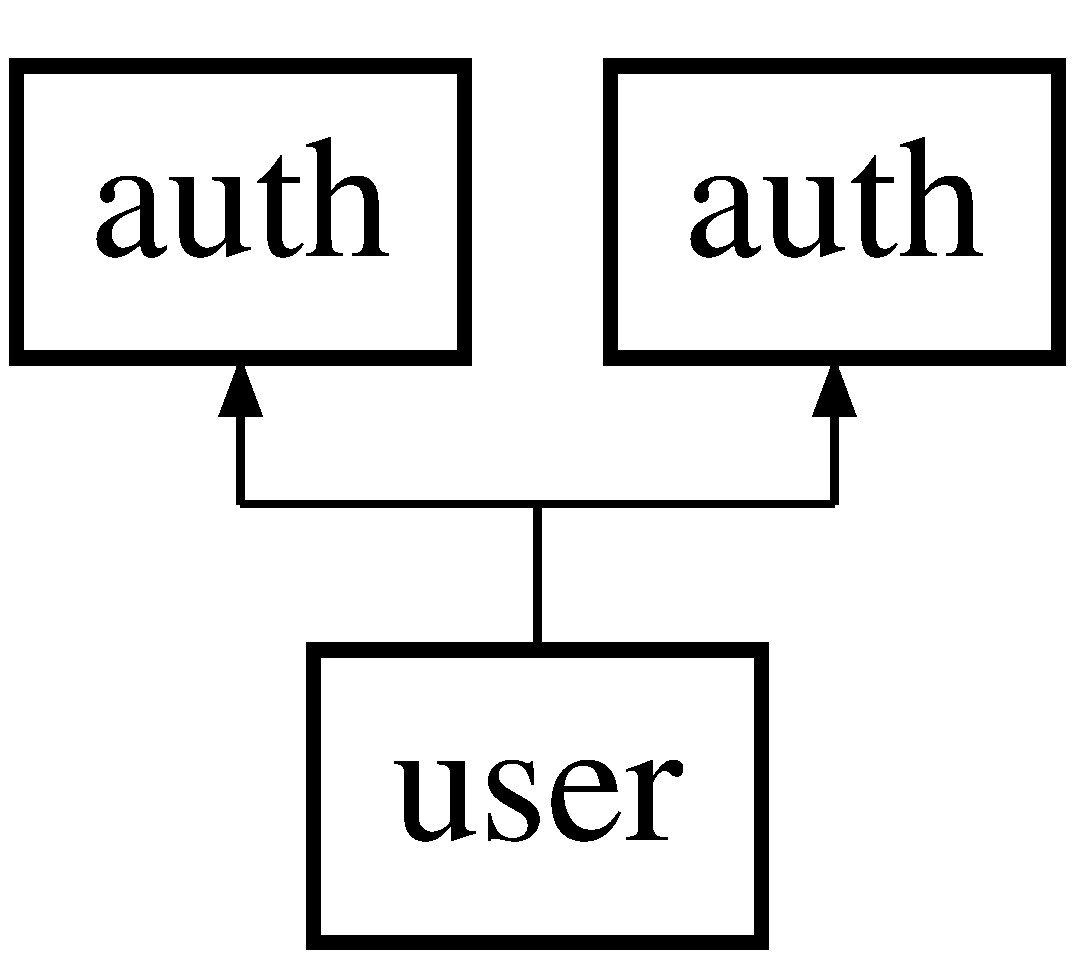
\includegraphics[height=2.000000cm]{classuser}
\end{center}
\end{figure}
\subsection*{Public Member Functions}
\begin{DoxyCompactItemize}
\item 
\hyperlink{classuser_acf59e1e14564ce949759964415069581}{\-\_\-\-\_\-construct} ()
\item 
\hyperlink{classuser_a0846994f392a18a32bfcae200cb33974}{login} (\$username, \$password)
\item 
\hyperlink{classuser_acb8e72f7d45579e3f07e071e06d11ac8}{logout} ()
\item 
\hyperlink{classuser_aad321ca58463f653b456dae243737c7e}{populate\-\_\-data} (\$id)
\item 
\hyperlink{classuser_a309159734946cdb67542dc0110055ae0}{remove\-\_\-data} ()
\item 
\hyperlink{classuser_a9538d09a879e3d85c9cedcc634df5751}{update\-\_\-lastlogin} ()
\item 
\hyperlink{classuser_a317fcb7a9feaf538c182b28fb7c9844c}{get\-\_\-lastlogin} ()
\end{DoxyCompactItemize}
\subsection*{Public Attributes}
\begin{DoxyCompactItemize}
\item 
\hypertarget{classuser_a60824fccae7197959b184fb04a6de2b9}{{\bfseries \$user} = array()}\label{classuser_a60824fccae7197959b184fb04a6de2b9}

\end{DoxyCompactItemize}


\subsection{Detailed Description}
This class handles all the user-\/related functions

\begin{DoxyAuthor}{Author}
piyush 
\end{DoxyAuthor}


Definition at line 10 of file user.\-php.



\subsection{Constructor \& Destructor Documentation}
\hypertarget{classuser_acf59e1e14564ce949759964415069581}{\index{user@{user}!\-\_\-\-\_\-construct@{\-\_\-\-\_\-construct}}
\index{\-\_\-\-\_\-construct@{\-\_\-\-\_\-construct}!user@{user}}
\subsubsection[{\-\_\-\-\_\-construct}]{\setlength{\rightskip}{0pt plus 5cm}user\-::\-\_\-\-\_\-construct (
\begin{DoxyParamCaption}
{}
\end{DoxyParamCaption}
)}}\label{classuser_acf59e1e14564ce949759964415069581}
Constructor of the class  type \$\-\_\-\-S\-E\-S\-S\-I\-O\-N The Superglobal session variable 

Definition at line 22 of file user.\-php.


\begin{DoxyCode}
22                                   \{
23         parent::\_\_construct();
24         global $\_SESSION;
25         \textcolor{keywordflow}{if} ($this->\hyperlink{classauth_ad5c908efc480a57e5625131348f4bf29}{check\_session}() == \textcolor{keyword}{true}) \{
26             \textcolor{comment}{//populate user data and set class variables to authenticated else normal}
27             $this->\hyperlink{classuser_aad321ca58463f653b456dae243737c7e}{populate\_data}($\_SESSION[\textcolor{stringliteral}{'id'}]);
28 
29             \textcolor{comment}{//Insert this recent activity time in the database}
30             $this->\hyperlink{classuser_a9538d09a879e3d85c9cedcc634df5751}{update\_lastlogin}();
31         \}
32     \}
\end{DoxyCode}


\subsection{Member Function Documentation}
\hypertarget{classuser_a317fcb7a9feaf538c182b28fb7c9844c}{\index{user@{user}!get\-\_\-lastlogin@{get\-\_\-lastlogin}}
\index{get\-\_\-lastlogin@{get\-\_\-lastlogin}!user@{user}}
\subsubsection[{get\-\_\-lastlogin}]{\setlength{\rightskip}{0pt plus 5cm}user\-::get\-\_\-lastlogin (
\begin{DoxyParamCaption}
{}
\end{DoxyParamCaption}
)}}\label{classuser_a317fcb7a9feaf538c182b28fb7c9844c}
This function is used to get the last login time of the user   \$db Instance of the db class \begin{DoxyReturn}{Returns}
integer Time\-Stamp of the last login 
\end{DoxyReturn}


Definition at line 113 of file user.\-php.


\begin{DoxyCode}
113                              \{
114         global $db;
115         $query = $db->query(\textcolor{stringliteral}{"select lastlogin from member where id="} . $this->
      \hyperlink{classuser}{user}[\textcolor{stringliteral}{'lastlogin'}]);
116 
117         $row = $db->fetch($query);
118 
119         \textcolor{keywordflow}{return} $row[\textcolor{stringliteral}{'lastlogin'}];
120     \}
\end{DoxyCode}
\hypertarget{classuser_a0846994f392a18a32bfcae200cb33974}{\index{user@{user}!login@{login}}
\index{login@{login}!user@{user}}
\subsubsection[{login}]{\setlength{\rightskip}{0pt plus 5cm}user\-::login (
\begin{DoxyParamCaption}
\item[{}]{\$username, }
\item[{}]{\$password}
\end{DoxyParamCaption}
)}}\label{classuser_a0846994f392a18a32bfcae200cb33974}
This function is used to log-\/in the user and populate the \$user variable with all the user data. Returns true if successful else false  array \$\-\_\-\-S\-E\-S\-S\-I\-O\-N The Superglobal Session variable 
\begin{DoxyParams}[1]{Parameters}
string & {\em \$username} & The username of the user \\
\hline
string & {\em \$password} & The password of the user \\
\hline
\end{DoxyParams}
\begin{DoxyReturn}{Returns}
boolean 
\end{DoxyReturn}


Definition at line 42 of file user.\-php.


\begin{DoxyCode}
42                                          \{
43         global $\_SESSION, $vanshavali;
44 
45         \textcolor{comment}{//Login}
46         $ret = $this->\hyperlink{classauth_a019d664334a621e770043d9fb4210836}{authenticate}($username, $password);
47 
48         \textcolor{comment}{//Populate the user array only if user has logged in}
49         \textcolor{keywordflow}{if} ($ret == \textcolor{keyword}{true} and ! is\_array($ret)) \{
50             $this->\hyperlink{classuser_aad321ca58463f653b456dae243737c7e}{populate\_data}($\_SESSION[\textcolor{stringliteral}{'id'}]);
51             \textcolor{comment}{//Drop a mail to admin regarding this}
52             $vanshavali->mailAdmin(\textcolor{stringliteral}{"mail.userloggedin.tpl"}, array(\textcolor{stringliteral}{"username"} => $username), \textcolor{stringliteral}{"User Logged in
      "});
53         \}
54 
55         \textcolor{comment}{//And return as it was previously doing before populate data was added}
56         \textcolor{keywordflow}{return} $ret;
57     \}
\end{DoxyCode}
\hypertarget{classuser_acb8e72f7d45579e3f07e071e06d11ac8}{\index{user@{user}!logout@{logout}}
\index{logout@{logout}!user@{user}}
\subsubsection[{logout}]{\setlength{\rightskip}{0pt plus 5cm}user\-::logout (
\begin{DoxyParamCaption}
{}
\end{DoxyParamCaption}
)}}\label{classuser_acb8e72f7d45579e3f07e071e06d11ac8}
This function is used to log-\/out the user and destroy the session \begin{DoxyReturn}{Returns}
null 
\end{DoxyReturn}


Definition at line 63 of file user.\-php.


\begin{DoxyCode}
63                       \{
64         \textcolor{comment}{//Remove all the session variables and remove user data}
65         $this->\hyperlink{classauth_a17089bfa7c3b9d0546f80ac9472dfc7b}{unauthenticate}();
66         $this->\hyperlink{classuser_a309159734946cdb67542dc0110055ae0}{remove\_data}();
67     \}
\end{DoxyCode}
\hypertarget{classuser_aad321ca58463f653b456dae243737c7e}{\index{user@{user}!populate\-\_\-data@{populate\-\_\-data}}
\index{populate\-\_\-data@{populate\-\_\-data}!user@{user}}
\subsubsection[{populate\-\_\-data}]{\setlength{\rightskip}{0pt plus 5cm}user\-::populate\-\_\-data (
\begin{DoxyParamCaption}
\item[{}]{\$id}
\end{DoxyParamCaption}
)}}\label{classuser_aad321ca58463f653b456dae243737c7e}
This function is used to populate the \$user variable with all the user data   \$db The instance of the db class 
\begin{DoxyParams}[1]{Parameters}
integer & {\em \$id} & The I\-D of the user to fetch the data of. \\
\hline
\end{DoxyParams}
\begin{DoxyReturn}{Returns}
null 
\end{DoxyReturn}


Definition at line 75 of file user.\-php.


\begin{DoxyCode}
75                                 \{
76         \textcolor{comment}{// Fill user variable with user data}
77         global $db;
78         $query = $db->query(\textcolor{stringliteral}{"Select * from member where id=$id"});
79         $row = $db->fetch($query);
80         $this->\hyperlink{classuser}{user} = $row;
81     \}
\end{DoxyCode}
\hypertarget{classuser_a309159734946cdb67542dc0110055ae0}{\index{user@{user}!remove\-\_\-data@{remove\-\_\-data}}
\index{remove\-\_\-data@{remove\-\_\-data}!user@{user}}
\subsubsection[{remove\-\_\-data}]{\setlength{\rightskip}{0pt plus 5cm}user\-::remove\-\_\-data (
\begin{DoxyParamCaption}
{}
\end{DoxyParamCaption}
)}}\label{classuser_a309159734946cdb67542dc0110055ae0}
This is the opposite of \hyperlink{classuser_aad321ca58463f653b456dae243737c7e}{populate\-\_\-data()} function. This function is used to remove the data from the \$user variable. \begin{DoxyReturn}{Returns}
null 
\end{DoxyReturn}


Definition at line 88 of file user.\-php.


\begin{DoxyCode}
88                            \{
89         \textcolor{comment}{//Remove data filled in user variable}
90         unset($this->\hyperlink{classuser}{user});
91         $this->\hyperlink{classuser}{user} = array();
92     \}
\end{DoxyCode}
\hypertarget{classuser_a9538d09a879e3d85c9cedcc634df5751}{\index{user@{user}!update\-\_\-lastlogin@{update\-\_\-lastlogin}}
\index{update\-\_\-lastlogin@{update\-\_\-lastlogin}!user@{user}}
\subsubsection[{update\-\_\-lastlogin}]{\setlength{\rightskip}{0pt plus 5cm}user\-::update\-\_\-lastlogin (
\begin{DoxyParamCaption}
{}
\end{DoxyParamCaption}
)}}\label{classuser_a9538d09a879e3d85c9cedcc634df5751}
This function is used to get the last activity time of the user   \$db Instance of the db class \begin{DoxyReturn}{Returns}
boolean True if successfull else false on unsuccessfull 
\end{DoxyReturn}


Definition at line 99 of file user.\-php.


\begin{DoxyCode}
99                                 \{
100         global $db;
101         \textcolor{keywordflow}{if} ($db->query(\textcolor{stringliteral}{"update member set lastlogin="} . time() . \textcolor{stringliteral}{" where id="} . $this->
      \hyperlink{classuser}{user}[\textcolor{stringliteral}{'id'}])) \{
102             \textcolor{keywordflow}{return} \textcolor{keyword}{true};
103         \} \textcolor{keywordflow}{else} \{
104             \textcolor{keywordflow}{return} \textcolor{keyword}{false};
105         \}
106     \}
\end{DoxyCode}


The documentation for this class was generated from the following file\-:\begin{DoxyCompactItemize}
\item 
user/user.\-php\end{DoxyCompactItemize}

\hypertarget{classvanshavali}{\section{vanshavali Class Reference}
\label{classvanshavali}\index{vanshavali@{vanshavali}}
}
\subsection*{Public Member Functions}
\begin{DoxyCompactItemize}
\item 
\hyperlink{classvanshavali_aee7778d3d1ccffd71859d14a811db6ee}{\-\_\-\-\_\-construct} ()
\item 
\hypertarget{classvanshavali_a317782832806850a2862914dbceef3c7}{{\bfseries get\-Headof\-Family} (\$family\-\_\-id=null)}\label{classvanshavali_a317782832806850a2862914dbceef3c7}

\item 
\hyperlink{classvanshavali_a0b6c7f158d1ffca2d8b69181a563f041}{distance\-From\-Top} (\$\hyperlink{classmember}{member}, \$samefamily=true)
\item 
\hypertarget{classvanshavali_a1673bbda002d16cf5596737bfc7a2369}{{\bfseries member\-Distance} (\$to, \$from)}\label{classvanshavali_a1673bbda002d16cf5596737bfc7a2369}

\item 
\hyperlink{classvanshavali_aac633019986e8d90d915ddafb772e26e}{calculate\-Relation} (\$from, \$to)
\item 
\hyperlink{classvanshavali_a1603b138202edbe428836fe91ddd23c4}{has\-Access} (\$who, \$whom)
\item 
\hyperlink{classvanshavali_a9bf310bbd46feca98b4c5b568575b6d4}{make\-Admin} (\$\hyperlink{classmember}{member})
\item 
\hyperlink{classvanshavali_a1d43abd82aa27e69dadbab48492801f0}{first\-Time\-Family} ()
\item 
\hyperlink{classvanshavali_a0b4f7c8e20e73e16bb9505ac0cae4817}{first\-Time} ()
\item 
\hyperlink{classvanshavali_a0ae3b4be4f88572f7780304504c39dbc}{addmember\-\_\-explicit} (\$membername, \$gender, \$familyid)
\item 
\hyperlink{classvanshavali_a0e2dc92ebdd355f1e995976f79285d1b}{addfamily} (\$name)
\item 
\hyperlink{classvanshavali_a91783e3f043278513c32ec2cca7f4c15}{getmember} (\$id)
\item 
\hyperlink{classvanshavali_a3de4f0b21ee02db0c12053d359543561}{register} (\$details)
\item 
\hyperlink{classvanshavali_aba5843e1d503de982e31f1366cef2abb}{mail} (\$template\-\_\-name, \$data, \$to, \$subject)
\item 
\hyperlink{classvanshavali_affea231be22eb26920637ec41b5dab04}{mail\-Admin} (\$template\-Name, \$data, \$subject)
\item 
\hyperlink{classvanshavali_a221c06bb6df817d86b784fddbada6855}{createstruct} (\$row)
\item 
\hyperlink{classvanshavali_a9f7d7e7137457aefbbd85ac33c5c1372}{getchild} (\$id)
\item 
\hyperlink{classvanshavali_a3ff1ca4043648fa9961a6fe2c1f94087}{getwife} (\$id)
\item 
\hyperlink{classvanshavali_aaff3d01d67e94c2371c39adabf1aba1e}{get\-Json\-\_\-new} (\$familyid=1)
\item 
\hyperlink{classvanshavali_adf31d7537f11e2235d6ffdcc7e8b11e7}{getchild\-\_\-new} (\$id)
\item 
\hyperlink{classvanshavali_ac63d3c3e833350cc3af38d9ba335be4c}{getwife\-\_\-new} (\$id)
\end{DoxyCompactItemize}
\subsection*{Public Attributes}
\begin{DoxyCompactItemize}
\item 
\hypertarget{classvanshavali_a8a53647182677d9f2f6f76a0dfd79b0f}{{\bfseries \$admin\-\_\-email}}\label{classvanshavali_a8a53647182677d9f2f6f76a0dfd79b0f}

\end{DoxyCompactItemize}
\subsection*{Private Member Functions}
\begin{DoxyCompactItemize}
\item 
\hyperlink{classvanshavali_aa0e3d9fa9b16e19fd150ed61781343f8}{comparerelation\-Array} (\$array)
\end{DoxyCompactItemize}
\subsection*{Private Attributes}
\begin{DoxyCompactItemize}
\item 
{\bfseries \$relation\-\_\-array}
\end{DoxyCompactItemize}


\subsection{Detailed Description}
This the core Class of the Family Tree and contains function to manage it.

\begin{DoxyAuthor}{Author}
piyush 
\end{DoxyAuthor}


Definition at line 11 of file vanshavali.\-php.



\subsection{Constructor \& Destructor Documentation}
\hypertarget{classvanshavali_aee7778d3d1ccffd71859d14a811db6ee}{\index{vanshavali@{vanshavali}!\-\_\-\-\_\-construct@{\-\_\-\-\_\-construct}}
\index{\-\_\-\-\_\-construct@{\-\_\-\-\_\-construct}!vanshavali@{vanshavali}}
\subsubsection[{\-\_\-\-\_\-construct}]{\setlength{\rightskip}{0pt plus 5cm}vanshavali\-::\-\_\-\-\_\-construct (
\begin{DoxyParamCaption}
{}
\end{DoxyParamCaption}
)}}\label{classvanshavali_aee7778d3d1ccffd71859d14a811db6ee}
Constructor of the class 

Definition at line 17 of file vanshavali.\-php.


\begin{DoxyCode}
17                                   \{
18         
19     \}
\end{DoxyCode}


\subsection{Member Function Documentation}
\hypertarget{classvanshavali_a0e2dc92ebdd355f1e995976f79285d1b}{\index{vanshavali@{vanshavali}!addfamily@{addfamily}}
\index{addfamily@{addfamily}!vanshavali@{vanshavali}}
\subsubsection[{addfamily}]{\setlength{\rightskip}{0pt plus 5cm}vanshavali\-::addfamily (
\begin{DoxyParamCaption}
\item[{}]{\$name}
\end{DoxyParamCaption}
)}}\label{classvanshavali_a0e2dc92ebdd355f1e995976f79285d1b}
This function is used to add family in the Tree. Returns the I\-D of the new family created or returns false if any error occured   \$db Instance of db class 
\begin{DoxyParams}[1]{Parameters}
string & {\em \$name} & The name of the Family \\
\hline
\end{DoxyParams}
\begin{DoxyReturn}{Returns}
integer I\-D of the new Family 
\end{DoxyReturn}


Definition at line 427 of file vanshavali.\-php.


\begin{DoxyCode}
427                               \{
428         global $db;
429         \textcolor{keywordflow}{if} ($db->query(\textcolor{stringliteral}{"insert into family (family\_name,ts) values('$name Family',"} . time() . \textcolor{stringliteral}{")"})) \{
430             \textcolor{keywordflow}{return} $db->last\_id();
431         \} \textcolor{keywordflow}{else} \{
432             \textcolor{keywordflow}{return} \textcolor{keyword}{false};
433         \}
434     \}
\end{DoxyCode}
\hypertarget{classvanshavali_a0ae3b4be4f88572f7780304504c39dbc}{\index{vanshavali@{vanshavali}!addmember\-\_\-explicit@{addmember\-\_\-explicit}}
\index{addmember\-\_\-explicit@{addmember\-\_\-explicit}!vanshavali@{vanshavali}}
\subsubsection[{addmember\-\_\-explicit}]{\setlength{\rightskip}{0pt plus 5cm}vanshavali\-::addmember\-\_\-explicit (
\begin{DoxyParamCaption}
\item[{}]{\$membername, }
\item[{}]{\$gender, }
\item[{}]{\$familyid}
\end{DoxyParamCaption}
)}}\label{classvanshavali_a0ae3b4be4f88572f7780304504c39dbc}
This special function is used to add member to the Tree without using any of the member class Returns the I\-D of the new member else false if any error occurred   \$db Instance of the db class 
\begin{DoxyParams}[1]{Parameters}
string & {\em \$membername} & The name of the new member to be added \\
\hline
integer & {\em \$gender} & The gender of the new member \\
\hline
integer & {\em \$familyid} & The Family I\-D of the new member \\
\hline
\end{DoxyParams}
\begin{DoxyReturn}{Returns}
integer I\-D of the new member created 
\end{DoxyReturn}


Definition at line 410 of file vanshavali.\-php.


\begin{DoxyCode}
410                                                                  \{
411         global $db;
412         \textcolor{keywordflow}{if} ($db->query(\textcolor{stringliteral}{"insert into member (membername,gender,family\_id) values
       ('$membername',$gender,$familyid)"})) \{
413             \textcolor{keywordflow}{return} mysql\_insert\_id();
414         \} \textcolor{keywordflow}{else} \{
415             \textcolor{keywordflow}{return} \textcolor{keyword}{false};
416         \}
417     \}
\end{DoxyCode}
\hypertarget{classvanshavali_aac633019986e8d90d915ddafb772e26e}{\index{vanshavali@{vanshavali}!calculate\-Relation@{calculate\-Relation}}
\index{calculate\-Relation@{calculate\-Relation}!vanshavali@{vanshavali}}
\subsubsection[{calculate\-Relation}]{\setlength{\rightskip}{0pt plus 5cm}vanshavali\-::calculate\-Relation (
\begin{DoxyParamCaption}
\item[{}]{\$from, }
\item[{}]{\$to}
\end{DoxyParamCaption}
)}}\label{classvanshavali_aac633019986e8d90d915ddafb772e26e}

\begin{DoxyParams}[1]{Parameters}
type & {\em \$from} & \\
\hline
type & {\em \$to} & \\
\hline
\end{DoxyParams}
\begin{DoxyReturn}{Returns}
string$\vert$boolean
\end{DoxyReturn}
Constants 0 brothers 1 mother 2 father 3 uncle chacha 4 aunty chachi 5 sister 6 grand father 7 grand mother 8 fufa (male) 9 fufa (female) 10 mama 11 mami 12 brother cousin 13 sister cousin 14 bhanja 15 bhanji 16 granchild 17 bhatiji 18 bhatija 19 Fore father 20 fore mother 21 grand son 22 grand daughter 23 bahoo 24 bahoo cousin 25 nata 26 nati 

Definition at line 288 of file vanshavali.\-php.


\begin{DoxyCode}
288                                                   \{
289         \textcolor{keywordflow}{if} ($from === $to) \{
290             \textcolor{keywordflow}{return} \textcolor{keyword}{false};
291         \}
292 
293         \textcolor{keywordflow}{if} ($from == null or $to == null) \{
294             \textcolor{keywordflow}{return} \textcolor{keyword}{false};
295         \}
296 
297         $from = $this->\hyperlink{classvanshavali_a91783e3f043278513c32ec2cca7f4c15}{getmember}($from);
298         $to = $this->\hyperlink{classvanshavali_a91783e3f043278513c32ec2cca7f4c15}{getmember}($to);
299 
300         \textcolor{comment}{//Get the parameters between them}
301         $relationparam = $this->memberDistance($to, $from);
302 
303         $result = $this->\hyperlink{classvanshavali_aa0e3d9fa9b16e19fd150ed61781343f8}{comparerelationArray}($relationparam);
304 
305         \textcolor{keywordflow}{if} (is\_array($result)) \{
306             \textcolor{keywordflow}{return} $result;
307         \} \textcolor{keywordflow}{else} \{
308             \textcolor{keywordflow}{return} print\_r($relationparam); \textcolor{comment}{//Just for development purpose}
309 \textcolor{comment}{//            return "Cannot determine relation";}
310         \}
311     \}
\end{DoxyCode}
\hypertarget{classvanshavali_aa0e3d9fa9b16e19fd150ed61781343f8}{\index{vanshavali@{vanshavali}!comparerelation\-Array@{comparerelation\-Array}}
\index{comparerelation\-Array@{comparerelation\-Array}!vanshavali@{vanshavali}}
\subsubsection[{comparerelation\-Array}]{\setlength{\rightskip}{0pt plus 5cm}vanshavali\-::comparerelation\-Array (
\begin{DoxyParamCaption}
\item[{}]{\$array}
\end{DoxyParamCaption}
)\hspace{0.3cm}{\ttfamily [private]}}}\label{classvanshavali_aa0e3d9fa9b16e19fd150ed61781343f8}

\begin{DoxyParams}[1]{Parameters}
type & {\em \$array} & \\
\hline
\end{DoxyParams}
\begin{DoxyReturn}{Returns}
boolean 
\end{DoxyReturn}


Definition at line 189 of file vanshavali.\-php.


\begin{DoxyCode}
189                                                   \{
190         \textcolor{comment}{//Initialize all the parameters}
191         $is\_child = $is\_parent = $is\_spouse = $gender = $sameFamily = $sameFather = $diffsex = 
      $levelDistance = \textcolor{keyword}{false};
192         $result = array();
193         $approx\_relation = \textcolor{keyword}{false};
194 
195 
196         \textcolor{comment}{//Now compare this array with all options that we have}
197         \textcolor{keywordflow}{foreach} ($this->relation\_array as $key => $singlerelation) \{
198             $is\_child = ($singlerelation[0] == $array[\textcolor{stringliteral}{'is\_child'}]);
199             $is\_parent = ($singlerelation[1] == $array[\textcolor{stringliteral}{'is\_parent'}]);
200             $is\_spouse = ($singlerelation[2] == $array[\textcolor{stringliteral}{'is\_spouse'}]);
201             $gender = ($singlerelation[3] == null ? \textcolor{keyword}{true} : ($singlerelation[3] == $array[\textcolor{stringliteral}{'gender'}]));
202             $sameFamily = ($singlerelation[4] == $array[\textcolor{stringliteral}{'sameFamily'}]);
203             $sameFather = ($singlerelation[5] == $array[\textcolor{stringliteral}{'sameFather'}]);
204             $diffsex = ($singlerelation[6] == null ? \textcolor{keyword}{true} : ($singlerelation[6] == $array[\textcolor{stringliteral}{'diffsex'}]));
205             $levelDistance = ($singlerelation[7] == $array[\textcolor{stringliteral}{'levelDistance'}]);
206 
207             \textcolor{comment}{//Check if this relation was approx relations}
208             \textcolor{keywordflow}{if} ($singlerelation[3] == null or $singlerelation[6] == null) \{
209                 $approx\_relation = \textcolor{keyword}{true};
210             \}
211 
212             \textcolor{keywordflow}{if} ($is\_child && $is\_parent && $is\_spouse && $gender &&
213                     $sameFamily && $sameFather && $diffsex && $levelDistance) \{
214 
215                 $result[] = array($singlerelation[8], $singlerelation[9], $approx\_relation);
216             \}
217 
218             \textcolor{comment}{//Reset the approx\_relation variable for the next relation}
219             $approx\_relation = \textcolor{keyword}{false};
220         \}
221 
222 
223         \textcolor{keywordflow}{if} (\textcolor{keyword}{sizeof}($result) == 0) \{
224             \textcolor{keywordflow}{return} \textcolor{keyword}{false}; \textcolor{comment}{// We couldn't find such relation}
225         \}
226 
227         \textcolor{comment}{//Check here if we have multiple values}
228         \textcolor{keywordflow}{if} (\textcolor{keyword}{sizeof}($result) == 1) \{
229             \textcolor{comment}{//Congrats, we heve only on relation to show.}
230             \textcolor{keywordflow}{return} $result[0];
231         \} elseif (\textcolor{keyword}{sizeof}($result) > 1) \{
232             \textcolor{comment}{//We have more than one relation which is matching}
233             \textcolor{comment}{//Select the one which is not approx}
234             $accurate\_relation = -1;
235             \textcolor{keywordflow}{foreach} ($result as $matched\_relation) \{
236                 \textcolor{keywordflow}{if} ($matched\_relation[2] == \textcolor{keyword}{false}) \{ \textcolor{comment}{//This says that it is not approximate relation}
237                     \textcolor{comment}{//Get out of the loop}
238                     $accurate\_relation = $matched\_relation;
239                     \textcolor{keywordflow}{break};
240                 \}
241             \}
242 
243             \textcolor{comment}{//Check if we have accurate relation}
244             \textcolor{keywordflow}{if} ($accurate\_relation == -1) \{
245                 \textcolor{keywordflow}{return} \textcolor{keyword}{false}; \textcolor{comment}{//Two many relations matching}
246             \} \textcolor{keywordflow}{else} \{
247                 \textcolor{keywordflow}{return} $accurate\_relation;
248             \}
249         \}
250     \}
\end{DoxyCode}
\hypertarget{classvanshavali_a221c06bb6df817d86b784fddbada6855}{\index{vanshavali@{vanshavali}!createstruct@{createstruct}}
\index{createstruct@{createstruct}!vanshavali@{vanshavali}}
\subsubsection[{createstruct}]{\setlength{\rightskip}{0pt plus 5cm}vanshavali\-::createstruct (
\begin{DoxyParamCaption}
\item[{}]{\$row}
\end{DoxyParamCaption}
)}}\label{classvanshavali_a221c06bb6df817d86b784fddbada6855}
This function is used to used to create structure to used by J\-I\-T. It takes input the array of a row from member table and converts it into the J\-I\-T structure. 
\begin{DoxyParams}[1]{Parameters}
array & {\em \$row} & \\
\hline
\end{DoxyParams}
\begin{DoxyReturn}{Returns}
array 
\end{DoxyReturn}


Definition at line 553 of file vanshavali.\-php.


\begin{DoxyCode}
553                                 \{
554         global $user;
555 
556         $obj = array();
557         $obj[\textcolor{stringliteral}{'id'}] = $row[\textcolor{stringliteral}{"id"}];
558         $obj[\textcolor{stringliteral}{'name'}] = trim($row[\textcolor{stringliteral}{'membername'}]) == \textcolor{stringliteral}{""} ? \textcolor{stringliteral}{"unknown"} : $row[\textcolor{stringliteral}{"membername"}];
559         $obj[\textcolor{stringliteral}{'data'}] = array(
560             \textcolor{stringliteral}{"dob"} => ($row[\textcolor{stringliteral}{'dob'}] ? strftime(\textcolor{stringliteral}{"%d/%m/%Y"}, $row[\textcolor{stringliteral}{'dob'}]) : \textcolor{stringliteral}{""}),
561             \textcolor{stringliteral}{"relationship\_status"} => ($row[\textcolor{stringliteral}{'relationship\_status'}] == 0 ? \textcolor{stringliteral}{"Single"} :
562                     \textcolor{stringliteral}{"Married"}),
563             \textcolor{stringliteral}{"relationship\_status\_id"} => $row[\textcolor{stringliteral}{'relationship\_status'}],
564             \textcolor{stringliteral}{"alive"} => ($row[\textcolor{stringliteral}{'alive'}] == 0 ? \textcolor{stringliteral}{"Deceased"} : \textcolor{stringliteral}{"Living"}),
565             \textcolor{stringliteral}{"gender"} => $row[\textcolor{stringliteral}{'gender'}],
566             \textcolor{stringliteral}{"alive\_id"} => $row[\textcolor{stringliteral}{'alive'}],
567             \textcolor{stringliteral}{"gaon"} => $row[\textcolor{stringliteral}{'gaon'}],
568             \textcolor{stringliteral}{'image'} => empty($row[\textcolor{stringliteral}{'profilepic'}]) ? \textcolor{stringliteral}{"common.png"} : $row[\textcolor{stringliteral}{'profilepic'}],
569             \textcolor{stringliteral}{'familyid'} => $row[\textcolor{stringliteral}{'family\_id'}]
570 \textcolor{comment}{//            'relation' => ($this->calculateRelation($row["id"], $user->user["id"]) ?
       $user->is\_authenticated() : "Login to view relation")}
571         );
572         \textcolor{keywordflow}{return} $obj;
573     \}
\end{DoxyCode}
\hypertarget{classvanshavali_a0b6c7f158d1ffca2d8b69181a563f041}{\index{vanshavali@{vanshavali}!distance\-From\-Top@{distance\-From\-Top}}
\index{distance\-From\-Top@{distance\-From\-Top}!vanshavali@{vanshavali}}
\subsubsection[{distance\-From\-Top}]{\setlength{\rightskip}{0pt plus 5cm}vanshavali\-::distance\-From\-Top (
\begin{DoxyParamCaption}
\item[{}]{\$member, }
\item[{}]{\$samefamily = {\ttfamily true}}
\end{DoxyParamCaption}
)}}\label{classvanshavali_a0b6c7f158d1ffca2d8b69181a563f041}

\begin{DoxyParams}[1]{Parameters}
type & {\em \$member} & \\
\hline
type & {\em \$samefamily} & \\
\hline
\end{DoxyParams}
\begin{DoxyReturn}{Returns}
int 
\end{DoxyReturn}


Definition at line 41 of file vanshavali.\-php.


\begin{DoxyCode}
41                                                                  \{
42 
43 
44         \textcolor{comment}{//While we are going up. We will first go to mother and then we will}
45         \textcolor{comment}{// to the father. This way we will be able to calculate relations for}
46         \textcolor{comment}{// female members of the family too.}
47 
48         \textcolor{keywordflow}{if} (!$samefamily) \{
49             \textcolor{comment}{//Since the family is not same. We will first switch to husband}
50             $member = $this->\hyperlink{classvanshavali_a91783e3f043278513c32ec2cca7f4c15}{getmember}($member->data[\textcolor{stringliteral}{'related\_to'}]);
51         \} \textcolor{comment}{//else we continue with normal execution}
52 
53         $distance = 0;
54         $mother = \textcolor{keyword}{true};
55         \textcolor{keywordflow}{while} (1) \{
56 
57             \textcolor{keywordflow}{if} ($mother) \{
58                 \textcolor{comment}{//Get father}
59                 \textcolor{comment}{//echo "\(\backslash\)nget the father to get mother. Father id = " . $member->data['sonof'];}
60                 $member = $this->\hyperlink{classvanshavali_a91783e3f043278513c32ec2cca7f4c15}{getmember}($member->data[\textcolor{stringliteral}{'sonof'}]);
61 
62                 \textcolor{keywordflow}{if} ($member === \textcolor{keyword}{false}) \{
63 \textcolor{comment}{//                    echo "\(\backslash\)nWent into first part break. Couldn't get the above given father";}
64                     \textcolor{keywordflow}{break};
65                 \}
66 
67                 \textcolor{comment}{//Get mother through him}
68                 $member = $this->\hyperlink{classvanshavali_a91783e3f043278513c32ec2cca7f4c15}{getmember}($member->data[\textcolor{stringliteral}{'related\_to'}]);
69 \textcolor{comment}{//                echo " \(\backslash\)nhere we should get the mother. Mother id = " . $member->id;}
70 
71                 $mother = \textcolor{keyword}{false}; \textcolor{comment}{//next turn is for father}
72 
73                 $distance++;
74             \} \textcolor{keywordflow}{else} \{
75 
76                 \textcolor{comment}{//Check for root. Last person will be male}
77                 \textcolor{keywordflow}{if} ($member == \textcolor{keyword}{false}) \{
78 \textcolor{comment}{//                    echo "\(\backslash\)nPrevious loop didn't return any member or there is no father to this member =
       " . $member->data['sonof'];}
79                     \textcolor{keywordflow}{break};
80                 \}
81                 \textcolor{comment}{//Previous loop was for mother. This one would be for father}
82                 $member = $this->\hyperlink{classvanshavali_a91783e3f043278513c32ec2cca7f4c15}{getmember}($member->data[\textcolor{stringliteral}{'related\_to'}]);
83 
84                 \textcolor{keywordflow}{if} ($member == \textcolor{keyword}{false}) \{
85 \textcolor{comment}{//                    echo " we can't find a husband to this wife.\(\backslash\)n";}
86                     \textcolor{keywordflow}{break};
87                 \}
88 
89                 $mother = \textcolor{keyword}{true}; \textcolor{comment}{//Next up is mother}
90 
91                 $distance++;
92             \}
93         \}
94 
95         \textcolor{keywordflow}{if} (!$samefamily) \{
96             \textcolor{comment}{//Since we switched to husband in the starting of the function,}
97             \textcolor{comment}{//We are by default one level down. Lets add to it.}
98             $distance++;
99         \}
100 
101         \textcolor{keywordflow}{return} $distance;
102     \}
\end{DoxyCode}
\hypertarget{classvanshavali_a0b4f7c8e20e73e16bb9505ac0cae4817}{\index{vanshavali@{vanshavali}!first\-Time@{first\-Time}}
\index{first\-Time@{first\-Time}!vanshavali@{vanshavali}}
\subsubsection[{first\-Time}]{\setlength{\rightskip}{0pt plus 5cm}vanshavali\-::first\-Time (
\begin{DoxyParamCaption}
{}
\end{DoxyParamCaption}
)}}\label{classvanshavali_a0b4f7c8e20e73e16bb9505ac0cae4817}
\$db \begin{DoxyReturn}{Returns}
boolean 
\end{DoxyReturn}


Definition at line 385 of file vanshavali.\-php.


\begin{DoxyCode}
385                                 \{
386         global $db;
387 
388         \textcolor{comment}{//Get the count on the number of members}
389         $query = $db->query(\textcolor{stringliteral}{"select count(*) membercount from member;"});
390 
391         $count = $db->fetch($query);
392 
393         \textcolor{keywordflow}{if} ($count[\textcolor{stringliteral}{'membercount'}] > 0) \{
394             \textcolor{keywordflow}{return} \textcolor{keyword}{false};
395         \} \textcolor{keywordflow}{else} \{
396             \textcolor{keywordflow}{return} \textcolor{keyword}{true};
397         \}
398     \}
\end{DoxyCode}
\hypertarget{classvanshavali_a1d43abd82aa27e69dadbab48492801f0}{\index{vanshavali@{vanshavali}!first\-Time\-Family@{first\-Time\-Family}}
\index{first\-Time\-Family@{first\-Time\-Family}!vanshavali@{vanshavali}}
\subsubsection[{first\-Time\-Family}]{\setlength{\rightskip}{0pt plus 5cm}vanshavali\-::first\-Time\-Family (
\begin{DoxyParamCaption}
{}
\end{DoxyParamCaption}
)}}\label{classvanshavali_a1d43abd82aa27e69dadbab48492801f0}
\$db \begin{DoxyReturn}{Returns}
boolean 
\end{DoxyReturn}


Definition at line 365 of file vanshavali.\-php.


\begin{DoxyCode}
365                                       \{
366         global $db;
367 
368         \textcolor{comment}{//Get the count on the number of members}
369         $query = $db->query(\textcolor{stringliteral}{"select count(*) membercount from family;"});
370 
371         $count = $db->fetch($query);
372 
373         \textcolor{keywordflow}{if} ($count[\textcolor{stringliteral}{'membercount'}] > 0) \{
374             \textcolor{keywordflow}{return} \textcolor{keyword}{false};
375         \} \textcolor{keywordflow}{else} \{
376             \textcolor{keywordflow}{return} \textcolor{keyword}{true};
377         \}
378     \}
\end{DoxyCode}
\hypertarget{classvanshavali_a9f7d7e7137457aefbbd85ac33c5c1372}{\index{vanshavali@{vanshavali}!getchild@{getchild}}
\index{getchild@{getchild}!vanshavali@{vanshavali}}
\subsubsection[{getchild}]{\setlength{\rightskip}{0pt plus 5cm}vanshavali\-::getchild (
\begin{DoxyParamCaption}
\item[{}]{\$id}
\end{DoxyParamCaption}
)}}\label{classvanshavali_a9f7d7e7137457aefbbd85ac33c5c1372}
This function is used to get the child of the given member to be fetched to the J\-I\-T. It fetches the details of the given member from the database and uses \hyperlink{classvanshavali_a221c06bb6df817d86b784fddbada6855}{createstruct()} to convert it into J\-I\-T structure.   \$db Instance of the db class 
\begin{DoxyParams}[1]{Parameters}
integer & {\em \$id} & Ihe of the member whose children are to be fetched \\
\hline
\end{DoxyParams}
\begin{DoxyReturn}{Returns}
array 
\end{DoxyReturn}


Definition at line 583 of file vanshavali.\-php.


\begin{DoxyCode}
583                            \{
584         global $db;
585         $finalarray = array();
586         $query = $db->query(\textcolor{stringliteral}{"select * from member where sonof=$id and dontshow=0"});
587         \textcolor{keywordflow}{while} ($row = $db->fetch($query)) \{
588             $obj = $this->\hyperlink{classvanshavali_a221c06bb6df817d86b784fddbada6855}{createstruct}($row);
589             $obj[\textcolor{stringliteral}{'children'}] = $this->\hyperlink{classvanshavali_a3ff1ca4043648fa9961a6fe2c1f94087}{getwife}($row[\textcolor{stringliteral}{'id'}]);
590             array\_push($finalarray, $obj);
591         \}
592         \textcolor{keywordflow}{return} $finalarray;
593     \}
\end{DoxyCode}
\hypertarget{classvanshavali_adf31d7537f11e2235d6ffdcc7e8b11e7}{\index{vanshavali@{vanshavali}!getchild\-\_\-new@{getchild\-\_\-new}}
\index{getchild\-\_\-new@{getchild\-\_\-new}!vanshavali@{vanshavali}}
\subsubsection[{getchild\-\_\-new}]{\setlength{\rightskip}{0pt plus 5cm}vanshavali\-::getchild\-\_\-new (
\begin{DoxyParamCaption}
\item[{}]{\$id}
\end{DoxyParamCaption}
)}}\label{classvanshavali_adf31d7537f11e2235d6ffdcc7e8b11e7}
This function is used to generate J\-S\-O\-N structure to be used in J\-I\-T of all children and subchildren under the passed member   \$db Instance of the db class 
\begin{DoxyParams}[1]{Parameters}
integer & {\em \$id} & I\-D of the member whose children are to be fetched \\
\hline
\end{DoxyParams}
\begin{DoxyReturn}{Returns}
array 
\end{DoxyReturn}


Definition at line 657 of file vanshavali.\-php.


\begin{DoxyCode}
657                                \{
658         global $db;
659         $finalarray = array();
660         $query = $db->query(\textcolor{stringliteral}{"select * from member where sonof=$id and dontshow=0"});
661         \textcolor{keywordflow}{while} ($row = $db->fetch($query)) \{
662             $obj = $this->infovisstruct($row);
663             $obj[\textcolor{stringliteral}{'children'}] = $this->\hyperlink{classvanshavali_a3ff1ca4043648fa9961a6fe2c1f94087}{getwife}($row[\textcolor{stringliteral}{'id'}]);
664             array\_push($finalarray, $obj);
665         \}
666         \textcolor{keywordflow}{return} $finalarray;
667     \}
\end{DoxyCode}
\hypertarget{classvanshavali_aaff3d01d67e94c2371c39adabf1aba1e}{\index{vanshavali@{vanshavali}!get\-Json\-\_\-new@{get\-Json\-\_\-new}}
\index{get\-Json\-\_\-new@{get\-Json\-\_\-new}!vanshavali@{vanshavali}}
\subsubsection[{get\-Json\-\_\-new}]{\setlength{\rightskip}{0pt plus 5cm}vanshavali\-::get\-Json\-\_\-new (
\begin{DoxyParamCaption}
\item[{}]{\$familyid = {\ttfamily 1}}
\end{DoxyParamCaption}
)}}\label{classvanshavali_aaff3d01d67e94c2371c39adabf1aba1e}
This function is used to get the members in J\-S\-O\-N format to be used with the J\-I\-T   \$db Instance of db class 
\begin{DoxyParams}[1]{Parameters}
integer & {\em \$familyid} & The I\-D of the family whose member are to be shown By default members of Family 1 are shown \\
\hline
\end{DoxyParams}
\begin{DoxyReturn}{Returns}
array$\vert$boolean 
\end{DoxyReturn}


Definition at line 628 of file vanshavali.\-php.


\begin{DoxyCode}
628                                         \{
629 
630         global $db;
631         $finalarray = array();
632         $query = $db->query(\textcolor{stringliteral}{"select * from member where sonof is null and dontshow=0 and gender=0"});
633         \textcolor{comment}{//Loop through all the members and feed the row data to a function}
634         \textcolor{comment}{//Loop will filter the data according to the gender and return}
635         \textcolor{comment}{//Keep adding the information to a final array}
636         $row = $db->fetch($query);
637 
638         \textcolor{comment}{//Now feed the row to function and in return get the array interface}
639         \textcolor{keywordflow}{if} (is\_array($row)) \{
640             $obj = $this->infovisstruct($row);
641             \textcolor{comment}{//$obj['children'] = $this->getwife($row['id']);}
642 
643             array\_push($finalarray, $obj);
644             \textcolor{keywordflow}{return} $finalarray;
645         \} \textcolor{keywordflow}{else} \{
646             \textcolor{keywordflow}{return} \textcolor{keyword}{false};
647         \}
648     \}
\end{DoxyCode}
\hypertarget{classvanshavali_a91783e3f043278513c32ec2cca7f4c15}{\index{vanshavali@{vanshavali}!getmember@{getmember}}
\index{getmember@{getmember}!vanshavali@{vanshavali}}
\subsubsection[{getmember}]{\setlength{\rightskip}{0pt plus 5cm}vanshavali\-::getmember (
\begin{DoxyParamCaption}
\item[{}]{\$id}
\end{DoxyParamCaption}
)}}\label{classvanshavali_a91783e3f043278513c32ec2cca7f4c15}
This function is used get the details about a member.   \$db Instance of the db class 
\begin{DoxyParams}[1]{Parameters}
integer & {\em \$id} & I\-D of the member whose details is to be fetched \\
\hline
\end{DoxyParams}
\begin{DoxyReturn}{Returns}

\end{DoxyReturn}


Definition at line 442 of file vanshavali.\-php.


\begin{DoxyCode}
442                             \{
443 
444         \textcolor{comment}{//Before doing anything. Lets check if we have everything}
445         \textcolor{keywordflow}{if} (empty($id)) \{
446             \textcolor{keywordflow}{return} \textcolor{keyword}{false};
447         \}
448 
449         global $db;
450         $query = $db->query(\textcolor{stringliteral}{"select id from member where id=$id"});
451         $ret = $db->fetch($query);
452 
453         \textcolor{comment}{//Check if we have such member or not}
454         \textcolor{keywordflow}{if} ($ret == \textcolor{keyword}{false}) \{
455             \textcolor{keywordflow}{return} \textcolor{keyword}{false};
456         \}
457 
458         \textcolor{comment}{//else proceed with normal execution}
459         $member = \textcolor{keyword}{new} \hyperlink{classmember}{member}($ret[\textcolor{stringliteral}{'id'}]);
460         \textcolor{keywordflow}{return} $member;
461     \}
\end{DoxyCode}
\hypertarget{classvanshavali_a3ff1ca4043648fa9961a6fe2c1f94087}{\index{vanshavali@{vanshavali}!getwife@{getwife}}
\index{getwife@{getwife}!vanshavali@{vanshavali}}
\subsubsection[{getwife}]{\setlength{\rightskip}{0pt plus 5cm}vanshavali\-::getwife (
\begin{DoxyParamCaption}
\item[{}]{\$id}
\end{DoxyParamCaption}
)}}\label{classvanshavali_a3ff1ca4043648fa9961a6fe2c1f94087}
This function is used to get the wife of the given member to be fetched into J\-I\-T. It fetches the details of the given member from the database and uses \hyperlink{classvanshavali_a221c06bb6df817d86b784fddbada6855}{createstruct()} to convert it into J\-I\-T structure.   \$db Instance of db class 
\begin{DoxyParams}[1]{Parameters}
integer & {\em \$id} & I\-D of the member whose wife is to be fetched \\
\hline
\end{DoxyParams}
\begin{DoxyReturn}{Returns}
array$\vert$null 
\end{DoxyReturn}


Definition at line 603 of file vanshavali.\-php.


\begin{DoxyCode}
603                           \{
604         global $db;
605         $finalarray = array();
606         $row = $db->get(\textcolor{stringliteral}{"select * from member where id in (select related\_to from member where id=$id)"});
607         $obj = array();
608         \textcolor{comment}{// Space Tree Object if he has a wife}
609         \textcolor{keywordflow}{if} ($row) \{
610             $obj = $this->\hyperlink{classvanshavali_a221c06bb6df817d86b784fddbada6855}{createstruct}($row);
611             $obj[\textcolor{stringliteral}{'children'}] = $this->\hyperlink{classvanshavali_a9f7d7e7137457aefbbd85ac33c5c1372}{getchild}($id);
612             array\_push($finalarray, $obj);
613             \textcolor{keywordflow}{return} $finalarray;
614         \} \textcolor{keywordflow}{else} \{
615             \textcolor{keywordflow}{return} NULL;
616         \}
617     \}
\end{DoxyCode}
\hypertarget{classvanshavali_ac63d3c3e833350cc3af38d9ba335be4c}{\index{vanshavali@{vanshavali}!getwife\-\_\-new@{getwife\-\_\-new}}
\index{getwife\-\_\-new@{getwife\-\_\-new}!vanshavali@{vanshavali}}
\subsubsection[{getwife\-\_\-new}]{\setlength{\rightskip}{0pt plus 5cm}vanshavali\-::getwife\-\_\-new (
\begin{DoxyParamCaption}
\item[{}]{\$id}
\end{DoxyParamCaption}
)}}\label{classvanshavali_ac63d3c3e833350cc3af38d9ba335be4c}
This function is used to generate J\-S\-O\-N structure to be used in J\-I\-T of the wife of the passed member   \$db Instance of db class 
\begin{DoxyParams}[1]{Parameters}
integer & {\em \$id} & I\-D of the member whose wife is to be fetched \\
\hline
\end{DoxyParams}
\begin{DoxyReturn}{Returns}
array$\vert$null 
\end{DoxyReturn}


Definition at line 676 of file vanshavali.\-php.


\begin{DoxyCode}
676                               \{
677         global $db;
678         $finalarray = array();
679         $row = $db->get(\textcolor{stringliteral}{"select * from member where id in (select related\_to from member where id=$id)"});
680         $obj = array();
681         \textcolor{comment}{// Space Tree Object if he has a wife}
682         \textcolor{keywordflow}{if} ($row) \{
683             $obj = $this->infovisstruct($row);
684             $obj[\textcolor{stringliteral}{'children'}] = $this->\hyperlink{classvanshavali_a9f7d7e7137457aefbbd85ac33c5c1372}{getchild}($id);
685             array\_push($finalarray, $obj);
686             \textcolor{keywordflow}{return} $finalarray;
687         \} \textcolor{keywordflow}{else} \{
688             \textcolor{keywordflow}{return} NULL;
689         \}
690     \}
\end{DoxyCode}
\hypertarget{classvanshavali_a1603b138202edbe428836fe91ddd23c4}{\index{vanshavali@{vanshavali}!has\-Access@{has\-Access}}
\index{has\-Access@{has\-Access}!vanshavali@{vanshavali}}
\subsubsection[{has\-Access}]{\setlength{\rightskip}{0pt plus 5cm}vanshavali\-::has\-Access (
\begin{DoxyParamCaption}
\item[{}]{\$who, }
\item[{}]{\$whom}
\end{DoxyParamCaption}
)}}\label{classvanshavali_a1603b138202edbe428836fe91ddd23c4}

\begin{DoxyParams}[1]{Parameters}
type & {\em \$who} & \\
\hline
type & {\em \$whom} & \\
\hline
\end{DoxyParams}
\begin{DoxyReturn}{Returns}
boolean 
\end{DoxyReturn}


Definition at line 319 of file vanshavali.\-php.


\begin{DoxyCode}
319                                            \{
320 
321         \textcolor{comment}{//accessArray}
322         $accessArray = array(12, 13, 15, 16, 0, 17, 1, 2);
324         \textcolor{comment}{//Basic things. User can edit is own information.}
325 
326         \textcolor{keywordflow}{if} ($who === $whom) \{
327             \textcolor{keywordflow}{return} \textcolor{keyword}{true};
328         \}
329 
330         \textcolor{comment}{//Make a check if the person is admin}
331         $mclass = \textcolor{keyword}{new} \hyperlink{classmember}{member}($who);
332         \textcolor{keywordflow}{if} ($mclass->isAdmin()) \{
333             \textcolor{comment}{//The person suggesting is admin. Just do it. :P}
334             \textcolor{keywordflow}{return} \textcolor{keyword}{true};
335         \}
336 
337         $relation = $this->\hyperlink{classvanshavali_aac633019986e8d90d915ddafb772e26e}{calculateRelation}($who, $whom);
338 
339         \textcolor{keywordflow}{if} (in\_array($relation, $accessArray)) \{
340             \textcolor{keywordflow}{return} \textcolor{keyword}{true};
341         \} \textcolor{keywordflow}{else} \{
342             \textcolor{keywordflow}{return} \textcolor{keyword}{false};
343         \}
344     \}
\end{DoxyCode}
\hypertarget{classvanshavali_aba5843e1d503de982e31f1366cef2abb}{\index{vanshavali@{vanshavali}!mail@{mail}}
\index{mail@{mail}!vanshavali@{vanshavali}}
\subsubsection[{mail}]{\setlength{\rightskip}{0pt plus 5cm}vanshavali\-::mail (
\begin{DoxyParamCaption}
\item[{}]{\$template\-\_\-name, }
\item[{}]{\$data, }
\item[{}]{\$to, }
\item[{}]{\$subject}
\end{DoxyParamCaption}
)}}\label{classvanshavali_aba5843e1d503de982e31f1366cef2abb}
This function is used to send a mail to an email\-I\-D. Returns false on error   \$template Instance of template class 
\begin{DoxyParams}[1]{Parameters}
string & {\em \$template\-\_\-name} & The name of the mail template to be used in the mail \\
\hline
array & {\em \$data} & The variables needed by the template used in the mail \\
\hline
string & {\em \$to} & Email\-I\-D of the Recipent \\
\hline
string & {\em \$subject} & The subject of the Mail \\
\hline
\end{DoxyParams}
\begin{DoxyReturn}{Returns}
boolean 
\end{DoxyReturn}


Definition at line 515 of file vanshavali.\-php.


\begin{DoxyCode}
515                                                         \{
516         global $template;
517         \textcolor{comment}{//Add Global variable of domain}
518         $user\_email = $this->admin\_email;
519 
520         \textcolor{comment}{//Fetch body from template}
521         $template->assign($data);
522         $body = $template->fetch($template\_name);
523 
524         \textcolor{comment}{//Mail Headers}
525         $headers = \textcolor{stringliteral}{"From: $user\_email\(\backslash\)r\(\backslash\)n"};
526         $headers .= \textcolor{stringliteral}{"Return-Path: $to\(\backslash\)r\(\backslash\)n"};
527         $headers .= \textcolor{stringliteral}{"X-Mailer: PHP/"} . phpversion() . \textcolor{stringliteral}{"\(\backslash\)r\(\backslash\)n"};
528         $headers .= \textcolor{stringliteral}{'MIME-Version: 1.0'} . \textcolor{stringliteral}{"\(\backslash\)n"};
529         $headers .= \textcolor{stringliteral}{'Content-type: text/html; UTF-8'} . \textcolor{stringliteral}{"\(\backslash\)r\(\backslash\)n"};
530 
531         \textcolor{keywordflow}{return} \hyperlink{classvanshavali_aba5843e1d503de982e31f1366cef2abb}{mail}($to, $subject, $body, $headers);
532     \}
\end{DoxyCode}
\hypertarget{classvanshavali_affea231be22eb26920637ec41b5dab04}{\index{vanshavali@{vanshavali}!mail\-Admin@{mail\-Admin}}
\index{mail\-Admin@{mail\-Admin}!vanshavali@{vanshavali}}
\subsubsection[{mail\-Admin}]{\setlength{\rightskip}{0pt plus 5cm}vanshavali\-::mail\-Admin (
\begin{DoxyParamCaption}
\item[{}]{\$template\-Name, }
\item[{}]{\$data, }
\item[{}]{\$subject}
\end{DoxyParamCaption}
)}}\label{classvanshavali_affea231be22eb26920637ec41b5dab04}

\begin{DoxyParams}[1]{Parameters}
type & {\em \$template\-Name} & \\
\hline
type & {\em \$data} & \\
\hline
type & {\em \$subject} & \\
\hline
\end{DoxyParams}
\begin{DoxyReturn}{Returns}
type 
\end{DoxyReturn}


Definition at line 541 of file vanshavali.\-php.


\begin{DoxyCode}
541                                                        \{
542 
543         \textcolor{keywordflow}{return} $this->\hyperlink{classvanshavali_aba5843e1d503de982e31f1366cef2abb}{mail}($templateName, $data, $this->admin\_email, $subject);
544     \}
\end{DoxyCode}
\hypertarget{classvanshavali_a9bf310bbd46feca98b4c5b568575b6d4}{\index{vanshavali@{vanshavali}!make\-Admin@{make\-Admin}}
\index{make\-Admin@{make\-Admin}!vanshavali@{vanshavali}}
\subsubsection[{make\-Admin}]{\setlength{\rightskip}{0pt plus 5cm}vanshavali\-::make\-Admin (
\begin{DoxyParamCaption}
\item[{}]{\$member}
\end{DoxyParamCaption}
)}}\label{classvanshavali_a9bf310bbd46feca98b4c5b568575b6d4}
\$db 
\begin{DoxyParams}[1]{Parameters}
type & {\em \$member} & \\
\hline
\end{DoxyParams}
\begin{DoxyReturn}{Returns}
type 
\end{DoxyReturn}


Definition at line 352 of file vanshavali.\-php.


\begin{DoxyCode}
352                                        \{
353         global $db;
354 
355         $query = $db->query(\textcolor{stringliteral}{"Update member set admin = 1 where id = $member"});
356 
357         \textcolor{keywordflow}{return} $query;
358     \}
\end{DoxyCode}
\hypertarget{classvanshavali_a3de4f0b21ee02db0c12053d359543561}{\index{vanshavali@{vanshavali}!register@{register}}
\index{register@{register}!vanshavali@{vanshavali}}
\subsubsection[{register}]{\setlength{\rightskip}{0pt plus 5cm}vanshavali\-::register (
\begin{DoxyParamCaption}
\item[{}]{\$details}
\end{DoxyParamCaption}
)}}\label{classvanshavali_a3de4f0b21ee02db0c12053d359543561}
This function is used to register a user in Family Tree. Returns false on error.   \$db Instance of db class   \$user Instance of user class 
\begin{DoxyParams}[1]{Parameters}
array & {\em \$details} & Array containing details about the new member \\
\hline
\end{DoxyParams}
\begin{DoxyReturn}{Returns}
boolean 
\end{DoxyReturn}


Definition at line 471 of file vanshavali.\-php.


\begin{DoxyCode}
471                                 \{
472         global $db, $user;
473 
474         \textcolor{comment}{//convert the password to md5 hash}
475         $details[1] = md5($details[1]);
476 
477         \textcolor{comment}{//The token for activation}
478         $token = $user->generate\_token();
479 
480         \textcolor{comment}{//Sql Statement}
481         \textcolor{keywordflow}{if} (!empty($details[8])) \{ \textcolor{comment}{//If member is not already connected to Family Tree then insert else
       update}
482             $sql = \textcolor{stringliteral}{"update member set
       membername='$details[9]',username='$details[0]',password='$details[1]',dob=$details[2],gender=$details[3],relationship\_status=$details[4],gaon='$details[5]',}
483 \textcolor{stringliteral}{    emailid='$details[6]',alive=1,aboutme='$details[7]',joined="} . time() . \textcolor{stringliteral}{",tokenforact='$token' where
       id=$details[8]"};
484         \} \textcolor{keywordflow}{else} \{
485             $sql = \textcolor{stringliteral}{"insert into member
       (membername,username,password,dob,gender,relationship\_status,gaon,emailid,alive,aboutme,joined,tokenforact, family\_id)}
486 \textcolor{stringliteral}{               
       values('$details[9]','$details[0]','$details[1]',$details[2],$details[3],$details[4],'$details[5]','$details[6]',1,'$details[7]',"} . time() . \textcolor{stringliteral}{",'$token', $details[10])"};
487         \}
488         \textcolor{comment}{//Finally execute the sql}
489         $ret = $db->query($sql);
490 
491         \textcolor{comment}{//Mail Options}
492         $mail\_options = array(
493             \textcolor{stringliteral}{'username'} => $details[0],
494             \textcolor{stringliteral}{'email'} => $details[6],
495             \textcolor{stringliteral}{'not\_connected'} => !empty($details[8]) ? \textcolor{keyword}{true} : \textcolor{keyword}{false}
496         );
497         \textcolor{keywordflow}{if} ($ret != \textcolor{keyword}{false}) \{
498             $this->\hyperlink{classvanshavali_aba5843e1d503de982e31f1366cef2abb}{mail}(\textcolor{stringliteral}{"mail.register.confirm.tpl"}, $mail\_options, $details[6], \textcolor{stringliteral}{'Welcome to Vanshavali
       | Email Confirmation'});
499             \textcolor{keywordflow}{return} \textcolor{keyword}{true};
500         \} \textcolor{keywordflow}{else} \{
501             trigger\_error(\textcolor{stringliteral}{"Cannot Connect to the database. Please try again by refreshing the page"}, 
      E\_USER\_ERROR);
502             \textcolor{keywordflow}{return} \textcolor{keyword}{false};
503         \}
504     \}
\end{DoxyCode}


\subsection{Member Data Documentation}
\hypertarget{classvanshavali_a55652a5f790bf930fa757ca553fd1cdb}{\index{vanshavali@{vanshavali}!\$relation\-\_\-array@{\$relation\-\_\-array}}
\index{\$relation\-\_\-array@{\$relation\-\_\-array}!vanshavali@{vanshavali}}
\subsubsection[{\$relation\-\_\-array}]{\setlength{\rightskip}{0pt plus 5cm}vanshavali\-::\$relation\-\_\-array\hspace{0.3cm}{\ttfamily [private]}}}\label{classvanshavali_a55652a5f790bf930fa757ca553fd1cdb}
{\bfseries Initial value\-:}
\begin{DoxyCode}
= array(
        array(\textcolor{keyword}{false}, \textcolor{keyword}{false}, \textcolor{keyword}{true}, MALE, \textcolor{keyword}{false}, \textcolor{keyword}{false}, \textcolor{keyword}{true}, -1, \textcolor{stringliteral}{"Wife"}, 12),
        array(\textcolor{keyword}{false}, \textcolor{keyword}{false}, \textcolor{keyword}{true}, FEMALE, \textcolor{keyword}{false}, \textcolor{keyword}{false}, \textcolor{keyword}{true}, -1, \textcolor{stringliteral}{"Husband"}, 13),
        array(\textcolor{keyword}{false}, \textcolor{keyword}{false}, \textcolor{keyword}{false}, FEMALE, \textcolor{keyword}{false}, \textcolor{keyword}{false}, \textcolor{keyword}{true}, -1, \textcolor{stringliteral}{"Brother-in-law (Devar)"}, 14),
        array(\textcolor{keyword}{true}, \textcolor{keyword}{false}, \textcolor{keyword}{false}, null, \textcolor{keyword}{true}, \textcolor{keyword}{false}, \textcolor{keyword}{false}, -2, \textcolor{stringliteral}{"Son"}, 15),
        array(\textcolor{keyword}{true}, \textcolor{keyword}{false}, \textcolor{keyword}{false}, null, \textcolor{keyword}{true}, \textcolor{keyword}{false}, \textcolor{keyword}{true}, -2, \textcolor{stringliteral}{"Daughter"}, 16),
        array(\textcolor{keyword}{false}, \textcolor{keyword}{false}, \textcolor{keyword}{false}, null, \textcolor{keyword}{true}, \textcolor{keyword}{true}, True, 0, \textcolor{stringliteral}{"Brother"}, 0),
        array(\textcolor{keyword}{false}, \textcolor{keyword}{false}, \textcolor{keyword}{false}, null, \textcolor{keyword}{true}, \textcolor{keyword}{true}, \textcolor{keyword}{false}, 0, \textcolor{stringliteral}{"Sister"}, 17),
        array(\textcolor{keyword}{false}, \textcolor{keyword}{true}, \textcolor{keyword}{false}, null, \textcolor{keyword}{false}, \textcolor{keyword}{false}, null, 1, \textcolor{stringliteral}{"Mother"}, 1),
        array(\textcolor{keyword}{false}, \textcolor{keyword}{true}, \textcolor{keyword}{false}, null, \textcolor{keyword}{true}, \textcolor{keyword}{false}, null, 2, \textcolor{stringliteral}{"Father"}, 2),
        array(\textcolor{keyword}{false}, \textcolor{keyword}{false}, \textcolor{keyword}{false}, null, \textcolor{keyword}{true}, \textcolor{keyword}{false}, \textcolor{keyword}{false}, 2, \textcolor{stringliteral}{"Chacha (Uncle)"}, 3),
        array(\textcolor{keyword}{false}, \textcolor{keyword}{false}, \textcolor{keyword}{false}, null, \textcolor{keyword}{false}, \textcolor{keyword}{false}, \textcolor{keyword}{true}, 1, \textcolor{stringliteral}{"Chachi (Aunt)"}, 4),
        array(\textcolor{keyword}{false}, \textcolor{keyword}{false}, \textcolor{keyword}{false}, null, \textcolor{keyword}{true}, \textcolor{keyword}{false}, \textcolor{keyword}{true}, 0, \textcolor{stringliteral}{"Cousin Sister"}, 5),
        array(\textcolor{keyword}{false}, \textcolor{keyword}{false}, \textcolor{keyword}{false}, null, \textcolor{keyword}{true}, \textcolor{keyword}{false}, \textcolor{keyword}{false}, 0, \textcolor{stringliteral}{"Cousin Brother"}, 6),
        array(\textcolor{keyword}{false}, \textcolor{keyword}{false}, \textcolor{keyword}{false}, null, \textcolor{keyword}{false}, \textcolor{keyword}{false}, \textcolor{keyword}{true}, -1, \textcolor{stringliteral}{"Bhabhi (Sister-in-law)"}, 7),
        array(\textcolor{keyword}{false}, \textcolor{keyword}{false}, \textcolor{keyword}{false}, null, \textcolor{keyword}{true}, \textcolor{keyword}{false}, \textcolor{keyword}{true}, -2, \textcolor{stringliteral}{"Bhatiji (Niece)"}, 8),
        array(\textcolor{keyword}{false}, \textcolor{keyword}{false}, \textcolor{keyword}{false}, null, \textcolor{keyword}{true}, \textcolor{keyword}{false}, \textcolor{keyword}{false}, -2, \textcolor{stringliteral}{"Bhatija (Niece)"}, 9),
        array(\textcolor{keyword}{false}, \textcolor{keyword}{false}, \textcolor{keyword}{false}, null, \textcolor{keyword}{false}, \textcolor{keyword}{false}, \textcolor{keyword}{true}, 3, \textcolor{stringliteral}{"Dadi Maa (GrandMother)"}, 10),
        array(\textcolor{keyword}{false}, \textcolor{keyword}{false}, \textcolor{keyword}{false}, null, \textcolor{keyword}{true}, \textcolor{keyword}{false}, \textcolor{keyword}{false}, 4, \textcolor{stringliteral}{"Dada Ji (GrandFather)"}, 11),
    )
\end{DoxyCode}


Definition at line 163 of file vanshavali.\-php.



The documentation for this class was generated from the following file\-:\begin{DoxyCompactItemize}
\item 
vanshavali/vanshavali.\-php\end{DoxyCompactItemize}

%--- End generated contents ---

% Index
\newpage
\phantomsection
\addcontentsline{toc}{chapter}{Index}
\printindex

\end{document}
